%\documentclass{beamer}
%\documentclass[slidestop,usepdftitle=false]{beamer}
\documentclass[english,10pt,table]{beamer}
%\documentclass[english,10pt,table,handout]{beamer}

% Copyright 2007 by Till Tantau
%
% This file may be distributed and/or modified
%
% 1. under the LaTeX Project Public License and/or
% 2. under the GNU Public License.
%
% See the file doc/licenses/LICENSE for more details.


% Common packages

\usepackage[english]{babel}
\usepackage[utf8]{vietnam}
%\usepackage{times}
\usefonttheme[onlymath]{serif}
\usecolortheme{default}
\usepackage{booktabs}
\usepackage{mathpartir}
\usepackage{listings}
\usepackage{pbox}
\mprset{flushleft}
\mode<article>
{
  \usepackage{times}
  \usepackage{mathptmx}
  \usepackage[left=1.5cm,right=6cm,top=1.5cm,bottom=3cm]{geometry}
}

\usepackage{hyperref}
\usepackage{tikz}
\usetikzlibrary{arrows,backgrounds}
%\tikzstyle{mnode}=[circle, draw, fill=black, inner sep=0pt, minimum width=4pt]
\usepackage{colortbl}
%\usepackage{yfonts}
\usepackage{translator} % comment this, if not available


% Common settings for all lectures in this course

\def\lecturename{Discrete Structures for Computing}

\title{\insertlecture}

\author{Huynh Tuong Nguyen, Tran Tuan Anh, Nguyen Ngoc Le}

\institute
{
  Faculty of Computer Science and Engineering\\
  University of Technology - VNUHCM \\
	\textcolor{blue}{htnguyen@hcmut.edu.vn}
}

\subject{Lecturer \lecturename}




% Beamer version theme settings

\useoutertheme[height=0pt,width=2cm,right]{sidebar}
\usecolortheme{rose,sidebartab}
\useinnertheme{circles}
\usefonttheme[only large]{structurebold}

\setbeamercolor{sidebar right}{bg=black!15}
\setbeamercolor{structure}{fg=blue}
\setbeamercolor{author}{parent=structure}

\setbeamerfont{title}{series=\normalfont,size=\LARGE}
\setbeamerfont{title in sidebar}{series=\bfseries}
\setbeamerfont{author in sidebar}{series=\bfseries}
\setbeamerfont*{item}{series=}
\setbeamerfont{frametitle}{size=}
\setbeamerfont{block title}{size=\small}
\setbeamerfont{subtitle}{size=\normalsize,series=\normalfont}

\setbeamertemplate{navigation symbols}{}
\setbeamertemplate{bibliography item}[book]
\setbeamertemplate{sidebar right}
{
  {\usebeamerfont{title in sidebar}%
    \vskip1.5em%
    \hskip3pt%
    \usebeamercolor[fg]{title in sidebar}%
    {\tiny\centering$\;$ Báo cáo Bài tập lớn}\par%
    \vskip1.25em%
  }%
  {%
    \hskip3pt%
    \usebeamercolor[fg]{author in sidebar}%
    \usebeamerfont{author in sidebar}%
    {\scriptsize\color{black}$\;\;\;\;$Nhóm 25}\par%
    \vskip1.25em%
  }%
  \hbox to2cm{\hss\insertlogo\hss}
  \vskip1.25em%
  \insertverticalnavigation{2cm}%
  \vfill
  \hbox to 2cm{\hfill\usebeamerfont{subsection in
      sidebar}\strut\usebeamercolor[fg]{subsection in
      sidebar}\insertshortlecture.\insertframenumber\hskip5pt}%
  \vskip3pt%
}%

\setbeamertemplate{title page}
{
  \vbox{}
  \vskip1em
  {\huge Cấu trúc rời rạc cho KHMT\par}
  {\usebeamercolor[fg]{title}\usebeamerfont{title}Báo cáo Bài tập lớn\par}%
   
  \vskip1em\par
  \emph{Ứng dụng thống kê khảo sát kết quả của bài tập online cho phép nộp bài nhiều lần}\
  \vskip0pt plus1filll
  \leftskip=0pt plus1fill
  \begin{tabular}{r l}
       GVHD: & \color{black} Huỳnh Tường Nguyên\\
       & \color{black} Trần Tuấn Anh\\
       & \color{black} Nguyễn Ngọc Lễ\\
       Nhóm: & \color{black} 25\\
       Thành viên: & \color{black} Tô Hòa -- 1910198 \\
       & \color{black} Trương Vĩnh Phước -- 1910473 \\
       & \color{black} Nguyễn Huỳnh Đức -- 1910137 \\
       & \color{black} Nguyễn Hoàng Trung -- 1910644 \\
       & \color{black} Ngô Lê Quốc Dũng -- 1910101 \\
       & \color{black} Lại Đức Anh Khoa -- 1910265 \\
  \end{tabular}
  \vskip1em
}

\logo{
\includegraphics[width=1.5cm]{hcmut.png}}



% Article version layout settings

\mode<article>

\makeatletter
\def\@listI{\leftmargin\leftmargini
  \parsep 0pt
  \topsep 5\p@   \@plus3\p@ \@minus5\p@
  \itemsep0pt}
\let\@listi=\@listI


\setbeamertemplate{frametitle}{\paragraph*{\insertframetitle\
    \ \small\insertframesubtitle}\ \par
}
\setbeamertemplate{frame end}{%
  \marginpar{\scriptsize\hbox to 1cm{\sffamily%
      \hfill\strut\insertshortlecture.\insertframenumber}\hrule height .2pt}}
\setlength{\marginparwidth}{1cm}
\setlength{\marginparsep}{4.5cm}

\def\@maketitle{\makechapter}

\def\makechapter{
  \newpage
  \null
  \vskip 2em%
  {%
    \parindent=0pt
    \raggedright
    \sffamily
    \vskip8pt
    {\fontsize{36pt}{36pt}\selectfont Chapter \insertshortlecture \par\vskip2pt}
    {\fontsize{24pt}{28pt}\selectfont \color{blue!50!black} \insertlecture\par\vskip4pt}
    {\Large\selectfont \color{blue!50!black} \insertsubtitle\par}
    \vskip10pt

    \normalsize\selectfont Print version of
    Lecturer \emph{\lecturename} of \@date\par\vskip1.5em
    \hfill Tran Vinh Tan, Faculty of CSE, University of Technology
  }
  \par
  \vskip 1.5em%
}

\let\origstartsection=\@startsection
\def\@startsection#1#2#3#4#5#6{%
  \origstartsection{#1}{#2}{#3}{#4}{#5}{#6\normalfont\sffamily\color{blue!50!black}\selectfont}}

\makeatother

\mode
<all>




% Typesetting Listings

\usepackage{listings}
\lstset{language=Java}

\alt<presentation>
{\lstset{%
  basicstyle=\footnotesize\ttfamily,
  commentstyle=\slshape\color{green!50!black},
  keywordstyle=\bfseries\color{blue!50!black},
  identifierstyle=\color{blue},
  stringstyle=\color{orange},
  escapechar=\#,
  emphstyle=\color{red}}
}
{
  \lstset{%
    basicstyle=\ttfamily,
    keywordstyle=\bfseries,
    commentstyle=\itshape,
    escapechar=\#,
    emphstyle=\bfseries\color{red}
  }
}



% Common theorem-like environments

\theoremstyle{example}
\newtheorem{exercise}[theorem]{\translate{Exercise}}


% New useful definitions:

\newbox\mytempbox
\newdimen\mytempdimen

\newcommand\includegraphicscopyright[3][]{%
  \leavevmode\vbox{\vskip3pt\raggedright\setbox\mytempbox=\hbox{\includegraphics[#1]{#2}}%
    \mytempdimen=\wd\mytempbox\box\mytempbox\par\vskip1pt%
    \fontsize{3}{3.5}\selectfont{\color{black!25}{\vbox{\hsize=\mytempdimen#3}}}\vskip3pt%
}}

\newenvironment{colortabular}[1]{\medskip\rowcolors[]{1}{blue!20}{blue!10}\tabular{#1}\rowcolor{blue!40}}{\endtabular\medskip}

\def\equad{\leavevmode\hbox{}\quad}

\newenvironment{greencolortabular}[1]
{\medskip\rowcolors[]{1}{green!50!black!20}{green!50!black!10}%
  \tabular{#1}\rowcolor{green!50!black!40}}%
{\endtabular\medskip}




\lecture[0]{Revision}{lecture-text}

\usepackage{pifont}
% Symbol definitions for these lists
\newcommand{\DingListSymbolA}{43}
\newcommand{\DingListSymbolB}{243}
\newcommand{\DingListSymbolC}{224}
\newcommand{\DingListSymbolD}{219}

% Boxed equation
\definecolor{LightYellow}{rgb}{1.,1.,.9}
\definecolor{LightRed}{rgb}{1.,.6,.6}


%%ensembles de nombres
\def\NP{$\mathcal{NP}$}
\def\N{\mathbb{N}}
\def\Z{\mathbb{Z}}
\def\R{\mathbb{R}}
\def\Q{\mathbb{Q}}

%\date[]{~~}

\everymath{\displaystyle \color{blue}}
%%%%%%%%%%%%%%%%%%%%%%%%%%%%%%%%%%%%%%%%%%%%%%%%%%%%%%%%%%%%%%%%%%%%%
%%%%%%%%%%%%%%%%%%%%%%%%%%%%%%%%%%%%%%%%%%%%%%%%%%%%%%%%%%%%%%%%%%%%%
\begin{document}
\frame{
\selectlanguage{english}
  \maketitle
}


%%%%%%%%%%%%%%%%%%%%%%%%%%%%%%%%%%%%%%%%%%%%%%%%%%%%%%%%%%%%%%%%%%%%%
%%%%%%%%%%%%%%%%%%%%%%%%%%%%%%%%%%%%%%%%%%%%%%%%%%%%%%%%%%%%%%%%%%%%%
%\section[Plan]{}
%\setcounter{tocdepth}{1}
\frame{ \tableofcontents}
%\setcounter{tocdepth}{5}
% to display left summary deeper and plan slide juste display section: add command \setcounter{tocdepth}{1} and then \setcounter{tocdepth}{10}  recompile twice or more again 

%%%%%%%%%%%%%%%%%%%%%%%%%%%%%%%%%%%%%%%%%%%%%%%%%%%%%%%%%%%%%%%%%%%%%
%%%%%%%%%%%%%%%%%%%%%%%%%%%%%%%%%%%%%%%%%%%%%%%%%%%%%%%%%%%%%%%%%%%%%
\section{Động cơ nghiên cứu}
\frame
{
\frametitle{Động cơ nghiên cứu}
\begin{itemize}
    \item ĐHQG TP.HCM triển khai giảng dạy trực tuyến
    \item Vai trò của phân tích và thống kê dữ liệu
\end{itemize}
}

\section{Mục tiêu}
\frame
{
\frametitle{Mục tiêu}
\begin{itemize}
    \item Đánh giá được các số liệu thống kê
    \item Làm quen với khai phá dữ liệu
\end{itemize}
}

%%%%%%%%%%%%%%%%%%%%%%%%%%%%%%%%%%%%%%%%%%%%%%%%%%%%%%%%%%%%%%%%%%%%%
%%%%%%%%%%%%%%%%%%%%%%%%%%%%%%%%%%%%%%%%%%%%%%%%%%%%%%%%%%%%%%%%%%%%%
\section{Nhiệm vụ}
\subsection{Thông tin chung}
\frame
{
\frametitle{Thông tin chung}
\begin{itemize}
    \item Nhóm: 25\\[6pt]
    \item Mã đề: $MD = 2907$\\[6pt]
    \item Bài tập cần làm: \textbf{1, 2, 3, 4, 5, 7, 9}\\[6pt]
    \item Bài tập làm thêm: \textbf{10, 11, 12}\\[6pt]
    \item Các file cần xử lý:
    \begin{itemize}
    	\item {\bf File 1:} CO1007\_TV\_HK192-Quiz 1.4-điểm.xlsx
	    \item {\bf File 2:} CO1007\_TV\_HK192-Quiz 1.5-điểm.xlsx	
    	\item {\bf File 3:} CO1007\_TV\_HK192-Quiz 3.3-điểm.xlsx
	    \item {\bf File 4:} CO1007\_TV\_HK192-Quiz 4.2-điểm.xlsx
    \end{itemize}
\end{itemize}
}

\subsection{Đọc dữ liệu}
\frame
{
\frametitle{Đọc dữ liệu}
Dữ liệu đầu vào gồm:
\begin{itemize}
    \item ID
    \item Status
    \item Start
    \item Finish
    \item Duration
    \item Total
    \item Q1 - Q10
\end{itemize}
}
%%%%%%%%%%%%%%%%%%%%%%%%%%%%%%%%%%%%%%%%%%%%%%%%%%%%%%%%%%%%%%%%%%%%%
%%%%%%%%%%%%%%%%%%%%%%%%%%%%%%%%%%%%%%%%%%%%%%%%%%%%%%%%%%%%%%%%%%%%%
\section{Xử lý dữ liệu}
\subsection{Bài 1}
\frame
{
\frametitle{Xác định số lượng sinh viên trên tập mẫu}
\begin{itemize}
    \item Ý tưởng thực hiện: $unique()$, $length()$
    \item Kết quả:\\
    \begin{center}
        \begin{tabular}{l l l}
             Quiz 1.4 & $\;$ & 344 sinh viên\\
             Quiz 1.5 & $\;$ & 343 sinh viên\\
             Quiz 3.3 & $\;$ & 280 sinh viên\\
             Quiz 4.2 & $\;$ & 260 sinh viên
        \end{tabular}
    \end{center}
\end{itemize}
}

%%%%%%%%%%%%%%%%%%%%%%%%%%%%%%%%%%%%%%%%%%%%%%%%%%%%%%%%%%%%%%%%%%%%
\subsection{Bài 2}
\frame
{
\frametitle{Nhóm câu hỏi liên quan đến điểm số sinh viên}
\framesubtitle{Xác định điểm tổng các bài làm}
\begin{itemize}
    \item Ý tưởng thực hiện: $sum()$
    \item Kết quả:\\
    \begin{center}
        \begin{tabular}{l l r}
             Quiz 1.4 & $\;$ & 5512.25 điểm\\
             Quiz 1.5 & $\;$ & 5668.5 điểm\\
             Quiz 3.3 & $\;$ & 3410 điểm\\
             Quiz 4.2 & $\;$ & 4406 điểm
        \end{tabular}
    \end{center}
\end{itemize}
}

\frame
{
\frametitle{Nhóm câu hỏi liên quan đến điểm số sinh viên}
\framesubtitle{Xác định điểm số thấp nhất}
\begin{itemize}
    \item Ý tưởng thực hiện: $min()$
    \item Kết quả:\\
    \begin{center}
        \begin{tabular}{l l r}
             Quiz 1.4 & $\;$ & 4.5 điểm\\
             Quiz 1.5 & $\;$ & 0.5 điểm\\
             Quiz 3.3 & $\;$ & 0 điểm\\
             Quiz 4.2 & $\;$ & 0 điểm
        \end{tabular}
    \end{center}
\end{itemize}
}

\frame
{
\frametitle{Nhóm câu hỏi liên quan đến điểm số sinh viên}
\framesubtitle{Xác định phổ theo số lần nộp bài của sinh viên có điểm số thấp nhất}
\begin{itemize}
    \item Ý tưởng thực hiện: $barplot()$
    \item Kết quả:\\
    \begin{center}
        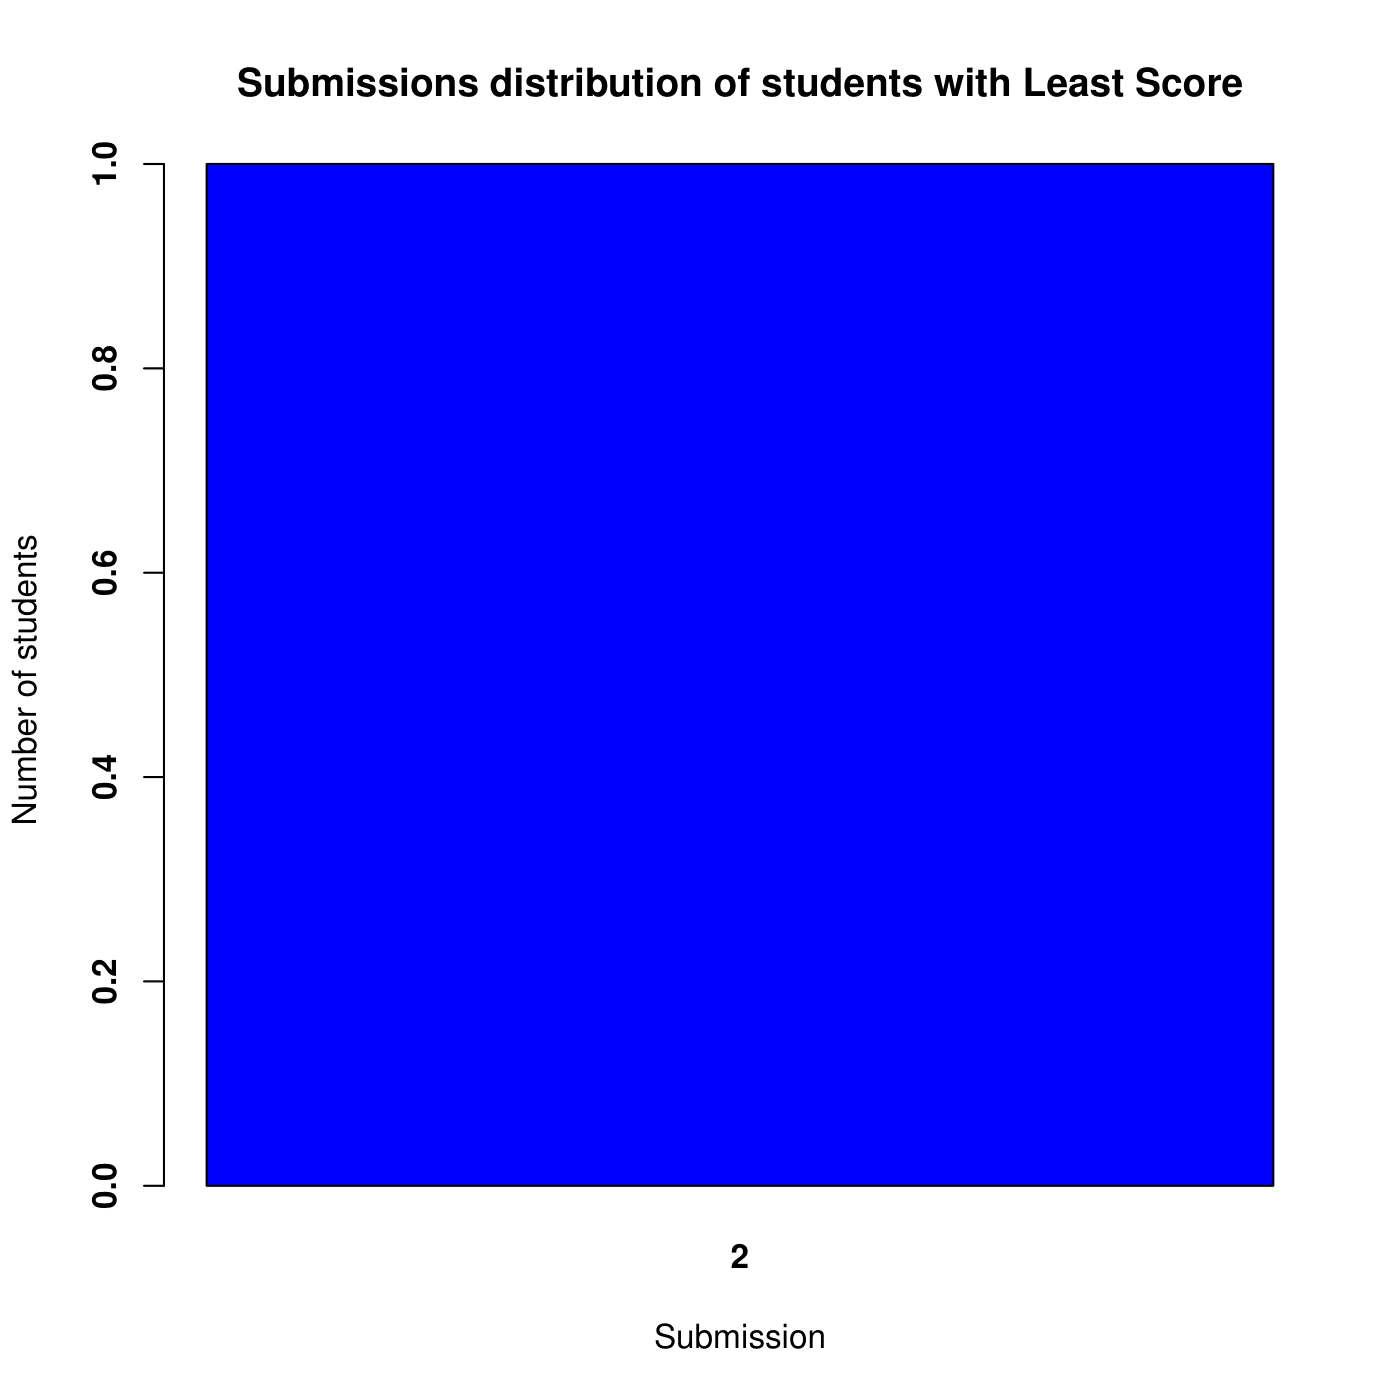
\includegraphics[width = 6 cm]{Images/img2-1-4.png}\\
        Kết quả của quiz 4.2
    \end{center}
\end{itemize}
}

\frame
{
\frametitle{Nhóm câu hỏi liên quan đến điểm số sinh viên}
\framesubtitle{Xác định điểm tổng kết thấp nhất}
\begin{itemize}
    \item Ý tưởng thực hiện: $min(), match(), unique()$
    \item Kết quả:\\
    \begin{center}
        \begin{tabular}{l l r}
             Quiz 1.4 & $\;$ & 8 điểm\\
             Quiz 1.5 & $\;$ & 7 điểm\\
             Quiz 3.3 & $\;$ & 8 điểm\\
             Quiz 4.2 & $\;$ & 7 điểm
        \end{tabular}
    \end{center}
\end{itemize}
}

\frame
{
\frametitle{Nhóm câu hỏi liên quan đến điểm số sinh viên}
\framesubtitle{Xác định phổ theo số lần nộp bài của sinh viên có điểm tổng kết thấp nhất}
\begin{itemize}
    \item Ý tưởng thực hiện: $barplot()$
    \item Kết quả:\\
    \begin{center}
        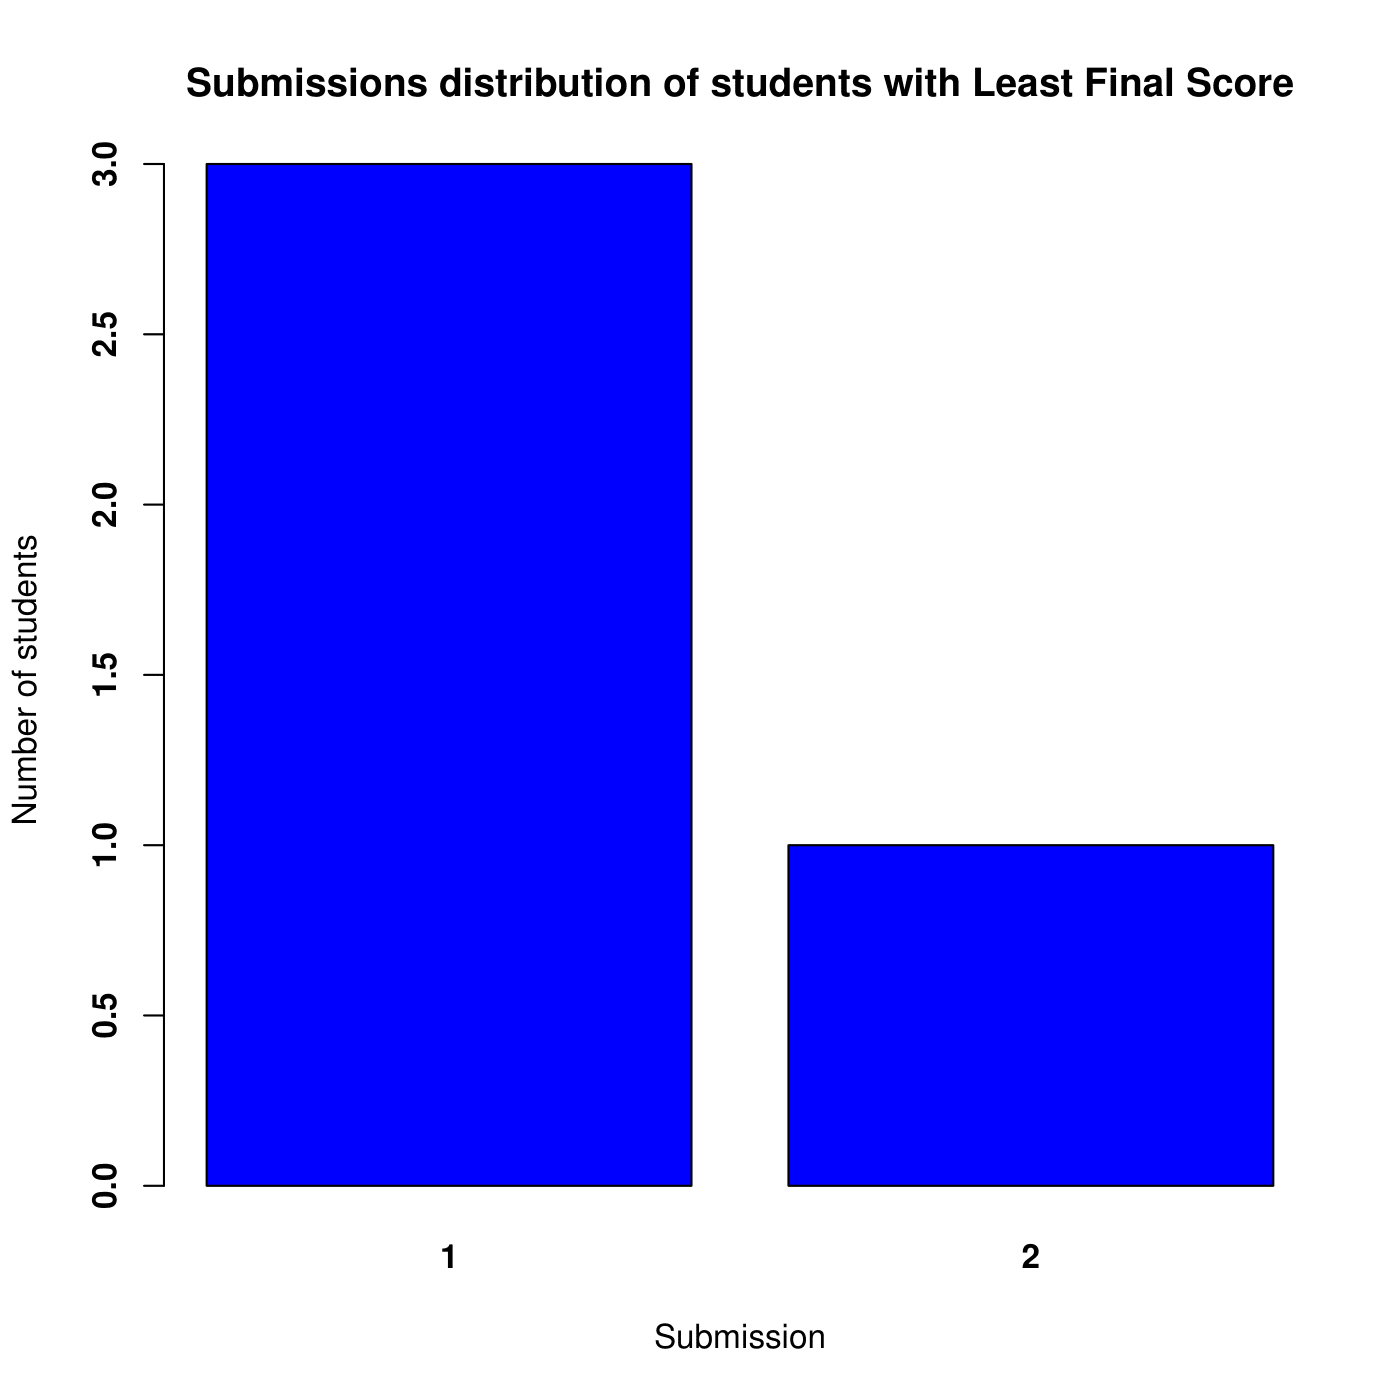
\includegraphics[width = 6 cm]{Images/img2-2-1.png}\\
        Kết quả của quiz 1.4
    \end{center}
\end{itemize}
}

\frame
{
\frametitle{Nhóm câu hỏi liên quan đến điểm số sinh viên}
\framesubtitle{Xác định điểm số cao nhất}
\begin{itemize}
    \item Ý tưởng thực hiện: $max()$
    \item Kết quả:\\
    \begin{center}
        \begin{tabular}{l l r}
             Quiz 1.4 & $\;$ & 10 điểm\\
             Quiz 1.5 & $\;$ & 10 điểm\\
             Quiz 3.3 & $\;$ & 10 điểm\\
             Quiz 4.2 & $\;$ & 10 điểm
        \end{tabular}
    \end{center}
\end{itemize}
}

\frame
{
\frametitle{Nhóm câu hỏi liên quan đến điểm số sinh viên}
\framesubtitle{Xác định phổ theo số lần nộp bài của sinh viên có điểm số cao nhất}
\begin{itemize}
    \item Ý tưởng thực hiện: $barplot()$
    \item Kết quả:\\
    \begin{center}
        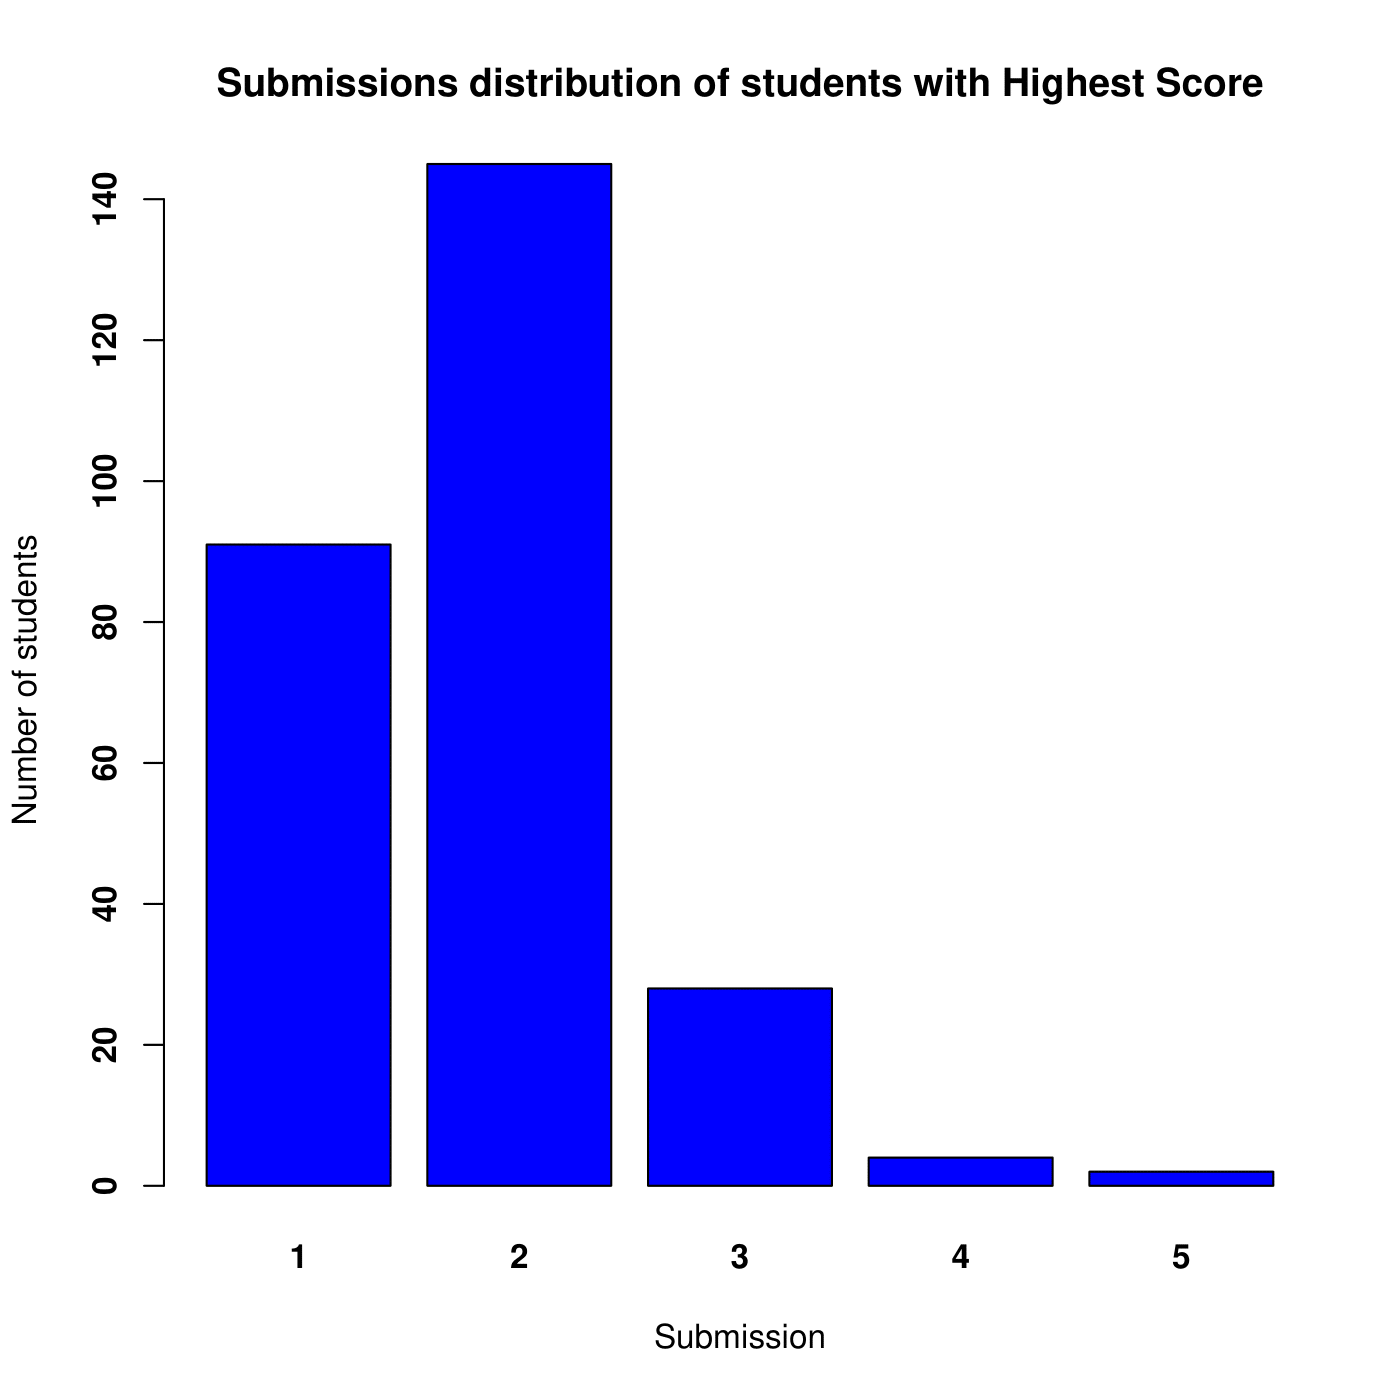
\includegraphics[width = 6 cm]{Images/img2-3-1.png}\\
        Kết quả của quiz 1.4
    \end{center}
\end{itemize}
}

\frame
{
\frametitle{Nhóm câu hỏi liên quan đến điểm số sinh viên}
\framesubtitle{Xác định điểm tổng kết cao nhất}
\begin{itemize}
    \item Ý tưởng thực hiện: $max()$
    \item Kết quả:\\
    \begin{center}
        \begin{tabular}{l l r}
             Quiz 1.4 & $\;$ & 10 điểm\\
             Quiz 1.5 & $\;$ & 10 điểm\\
             Quiz 3.3 & $\;$ & 10 điểm\\
             Quiz 4.2 & $\;$ & 10 điểm
        \end{tabular}
    \end{center}
\end{itemize}
}

\frame
{
\frametitle{Nhóm câu hỏi liên quan đến điểm số sinh viên}
\framesubtitle{Xác định phổ theo số lần nộp bài của sinh viên có điểm tổng kết cao nhất}
\begin{itemize}
    \item Ý tưởng thực hiện: $barplot()$
    \item Kết quả:\\
    \begin{center}
        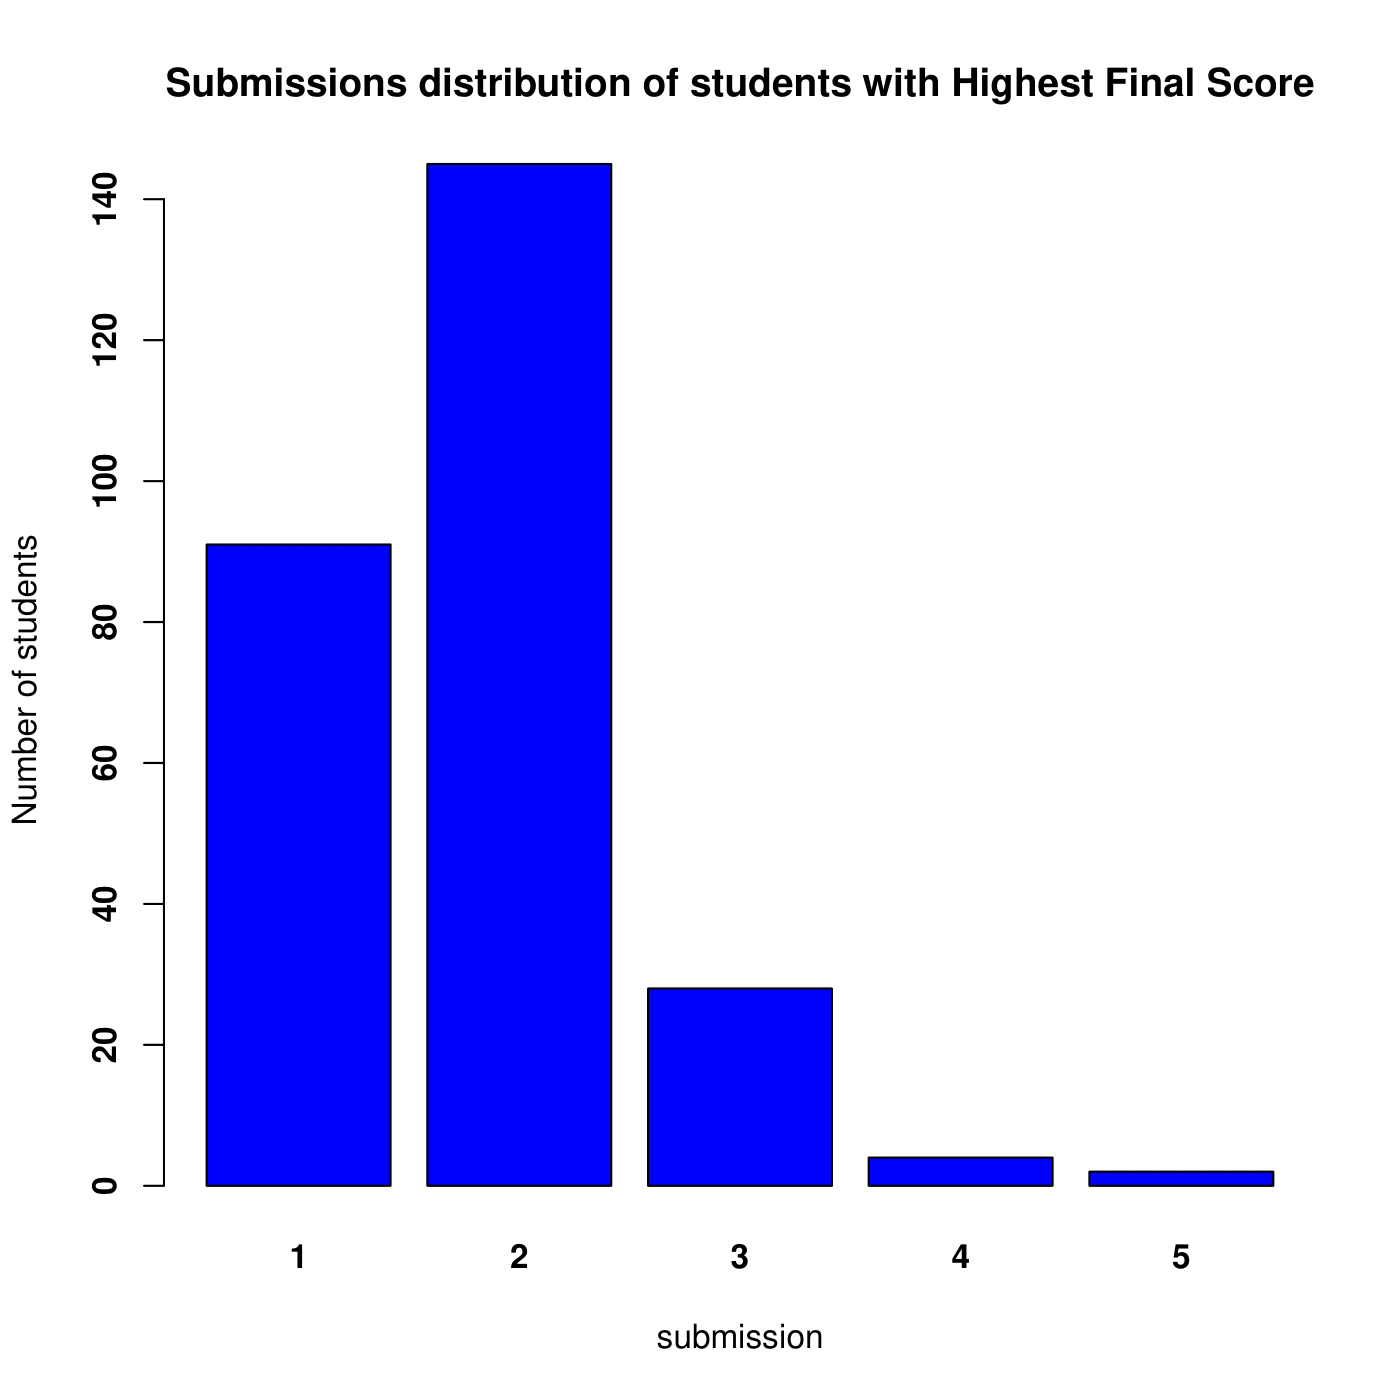
\includegraphics[width = 6 cm]{Images/img2-4-1.png}\\
        Kết quả của quiz 1.4
    \end{center}
\end{itemize}
}

\frame
{
\frametitle{Nhóm câu hỏi liên quan đến điểm số sinh viên}
\framesubtitle{Xác định điểm số trung bình}
\begin{itemize}
    \item Ý tưởng thực hiện: $mean()$
    \item Kết quả:\\
    \begin{center}
        \begin{tabular}{l l r}
             Quiz 1.4 & $\;$ & 9.8 điểm\\
             Quiz 1.5 & $\;$ & 9.8 điểm\\
             Quiz 3.3 & $\;$ & 9.9 điểm\\
             Quiz 4.2 & $\;$ & 9.8 điểm
        \end{tabular}
    \end{center}
\end{itemize}
}

\frame
{
\frametitle{Nhóm câu hỏi liên quan đến điểm số sinh viên}
\framesubtitle{Xác định số lượng sinh viên có điểm số trung bình}
\begin{itemize}
    \item Ý tưởng thực hiện: $subset(), length()$
    \item Kết quả:\\
    \begin{center}
        \begin{tabular}{l l r}
             Quiz 1.4 & $\;$ & 0 sinh viên\\
             Quiz 1.5 & $\;$ & 0 sinh viên\\
             Quiz 3.3 & $\;$ & 0 sinh viên\\
             Quiz 4.2 & $\;$ & 0 sinh viên
        \end{tabular}
    \end{center}
\end{itemize}
}

\frame
{
\frametitle{Nhóm câu hỏi liên quan đến điểm số sinh viên}
\framesubtitle{Tính trung vị, cực đại, cực mẫu}
\begin{itemize}
    \item Ý tưởng thực hiện: $median(), max(), min()$
    \item Kết quả:\\
    \begin{center}
        \begin{tabular}{l l c c c}
             & & Trung vị & Cực đại & Cực tiểu\\
             Quiz 1.4 & $\;$ & 9.67 & 10 & 4.5\\
             Quiz 1.5 & $\;$ & 9.5 & 10 & 0.5\\
             Quiz 3.3 & $\;$ & 10 & 10 & 0\\
             Quiz 4.2 & $\;$ & 9.5 & 10 & 0
        \end{tabular}
    \end{center}
\end{itemize}
}

\frame
{
\frametitle{Nhóm câu hỏi liên quan đến điểm số sinh viên}
\framesubtitle{Đo mức độ phân tán của điểm số xung quang giá trị trung bình}
\begin{itemize}
    \item Ý tưởng thực hiện: $var(), sd()$
    \item Kết quả:\\
    \begin{center}
        \begin{tabular}{l l c c c}
             & & Phương sai & Độ lệch chuẩn\\
             Quiz 1.4 & $\;$ & 0.8145266 & 0.9025113\\
             Quiz 1.5 & $\;$ & 1.238846 & 1.113034\\
             Quiz 3.3 & $\;$ & 0.6682011 & 0.8174357\\
             Quiz 4.2 & $\;$ & 1.874935 & 1.369283
        \end{tabular}
    \end{center}
\end{itemize}
}

\frame
{
\frametitle{Nhóm câu hỏi liên quan đến điểm số sinh viên}
\framesubtitle{Tính độ méo lệch, độ nhọn}
\begin{itemize}
    \item Ý tưởng thực hiện: $skewness(), kurtosis()$
    \item Kết quả:\\
    \begin{center}
        \begin{tabular}{l l c c c}
             & & Độ méo lệch & Độ nhọn\\
             Quiz 1.4 & $\;$ & -1.507457 & 5.730385\\
             Quiz 1.5 & $\;$ & -2.62223 & 15.32753\\
             Quiz 3.3 & $\;$ & -6.303646 & 64.30899\\
             Quiz 4.2 & $\;$ & -1.601421 & 7.084802
        \end{tabular}
    \end{center}
\end{itemize}
}

\frame
{
\frametitle{Nhóm câu hỏi liên quan đến điểm số sinh viên}
\framesubtitle{Xác định tứ phân vị thứ nhất - thứ ba}
\begin{itemize}
    \item Ý tưởng thực hiện: $quantile()$
    \item Kết quả:\\
    \begin{center}
        \begin{tabular}{l l c c c}
             & & Thứ nhất & Thứ ba\\
             Quiz 1.4 & $\;$ & 9 & 10\\
             Quiz 1.5 & $\;$ & 9 & 10\\
             Quiz 3.3 & $\;$ & 9 & 10\\
             Quiz 4.2 & $\;$ & 8 & 10
        \end{tabular}
    \end{center}
\end{itemize}
}

\frame
{
\frametitle{Nhóm câu hỏi liên quan đến điểm số sinh viên}
\framesubtitle{Xác định số lượng sinh viên có điểm số nằm trong 2 mức điểm cao nhất}
\begin{itemize}
    \item Ý tưởng thực hiện: $max(), subset(), length()$
    \item Kết quả:\\
    \begin{center}
        \begin{tabular}{l l c c c}
             Quiz 1.4 & $\;$ & 287 sinh viên\\
             Quiz 1.5 & $\;$ & 297 sinh viên\\
             Quiz 3.3 & $\;$ & 277 sinh viên\\
             Quiz 4.2 & $\;$ & 222 sinh viên
        \end{tabular}
    \end{center}
\end{itemize}
}

\frame
{
\frametitle{Nhóm câu hỏi liên quan đến điểm số sinh viên}
\framesubtitle{Xác định phổ theo số lần nộp bài của sinh viên có điểm tổng kết nằm ở 2 mức điểm cao nhất}
\begin{itemize}
    \item Ý tưởng thực hiện: $barplot()$
    \item Kết quả:\\
    \begin{center}
        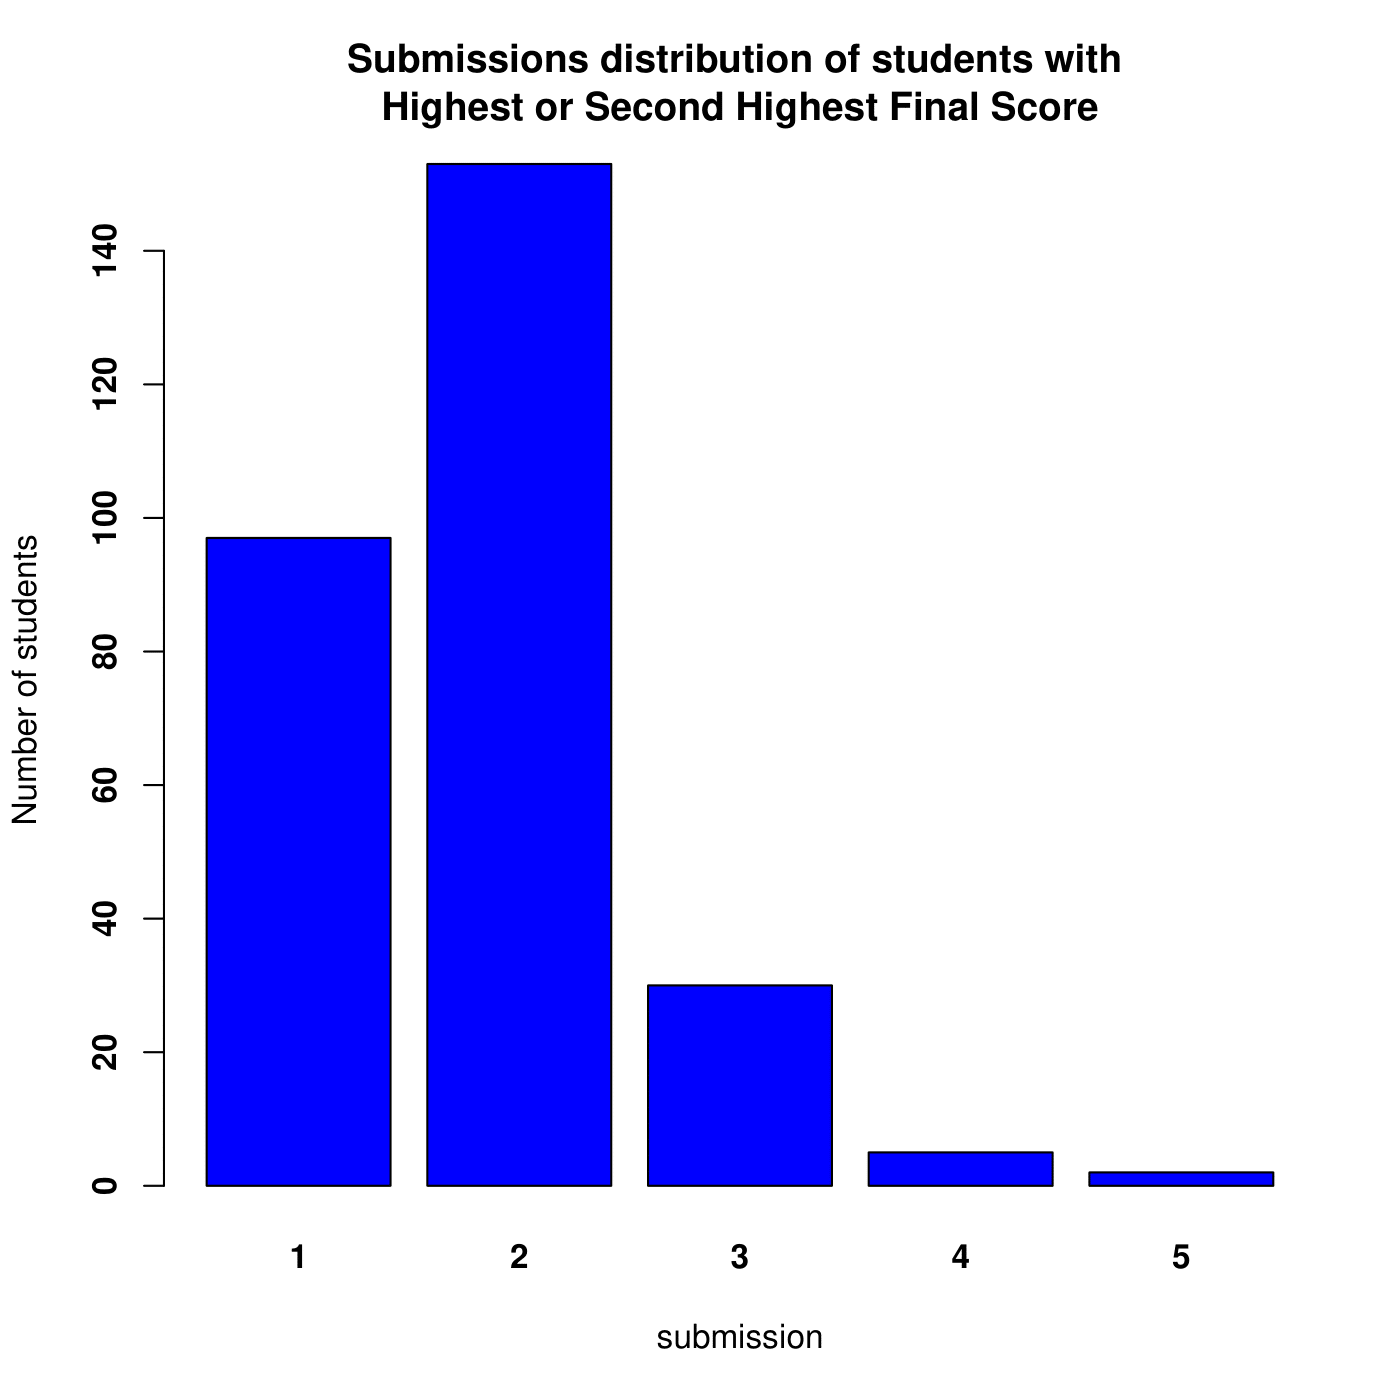
\includegraphics[width = 6 cm]{Images/img2-5-1.png}\\
        Kết quả của quiz 1.4
    \end{center}
\end{itemize}
}

\frame
{
\frametitle{Nhóm câu hỏi liên quan đến điểm số sinh viên}
\framesubtitle{Xác định số lượng sinh viên có điểm tổng kết ở mức k cao nhất}
\begin{itemize}
    \item Ý tưởng thực hiện: $unique(), order(), subset(), nrow()$
    \item Kết quả: giả sử với k = 2\\
    \begin{center}
        \begin{tabular}{l l c c c}
             Quiz 1.4 & $\;$ & 17 sinh viên\\
             Quiz 1.5 & $\;$ & 26 sinh viên\\
             Quiz 3.3 & $\;$ & 17 sinh viên\\
             Quiz 4.2 & $\;$ & 21 sinh viên
        \end{tabular}
    \end{center}
\end{itemize}
}

\frame
{
\frametitle{Nhóm câu hỏi liên quan đến điểm số sinh viên}
\framesubtitle{Xác định phổ theo số lần nộp bài của các sinh viên có điểm số tổng kết ở mức điểm cao thứ k}
\begin{itemize}
    \item Ý tưởng thực hiện: $barplot()$
    \item Kết quả: giả sử k = 2\\
    \begin{center}
        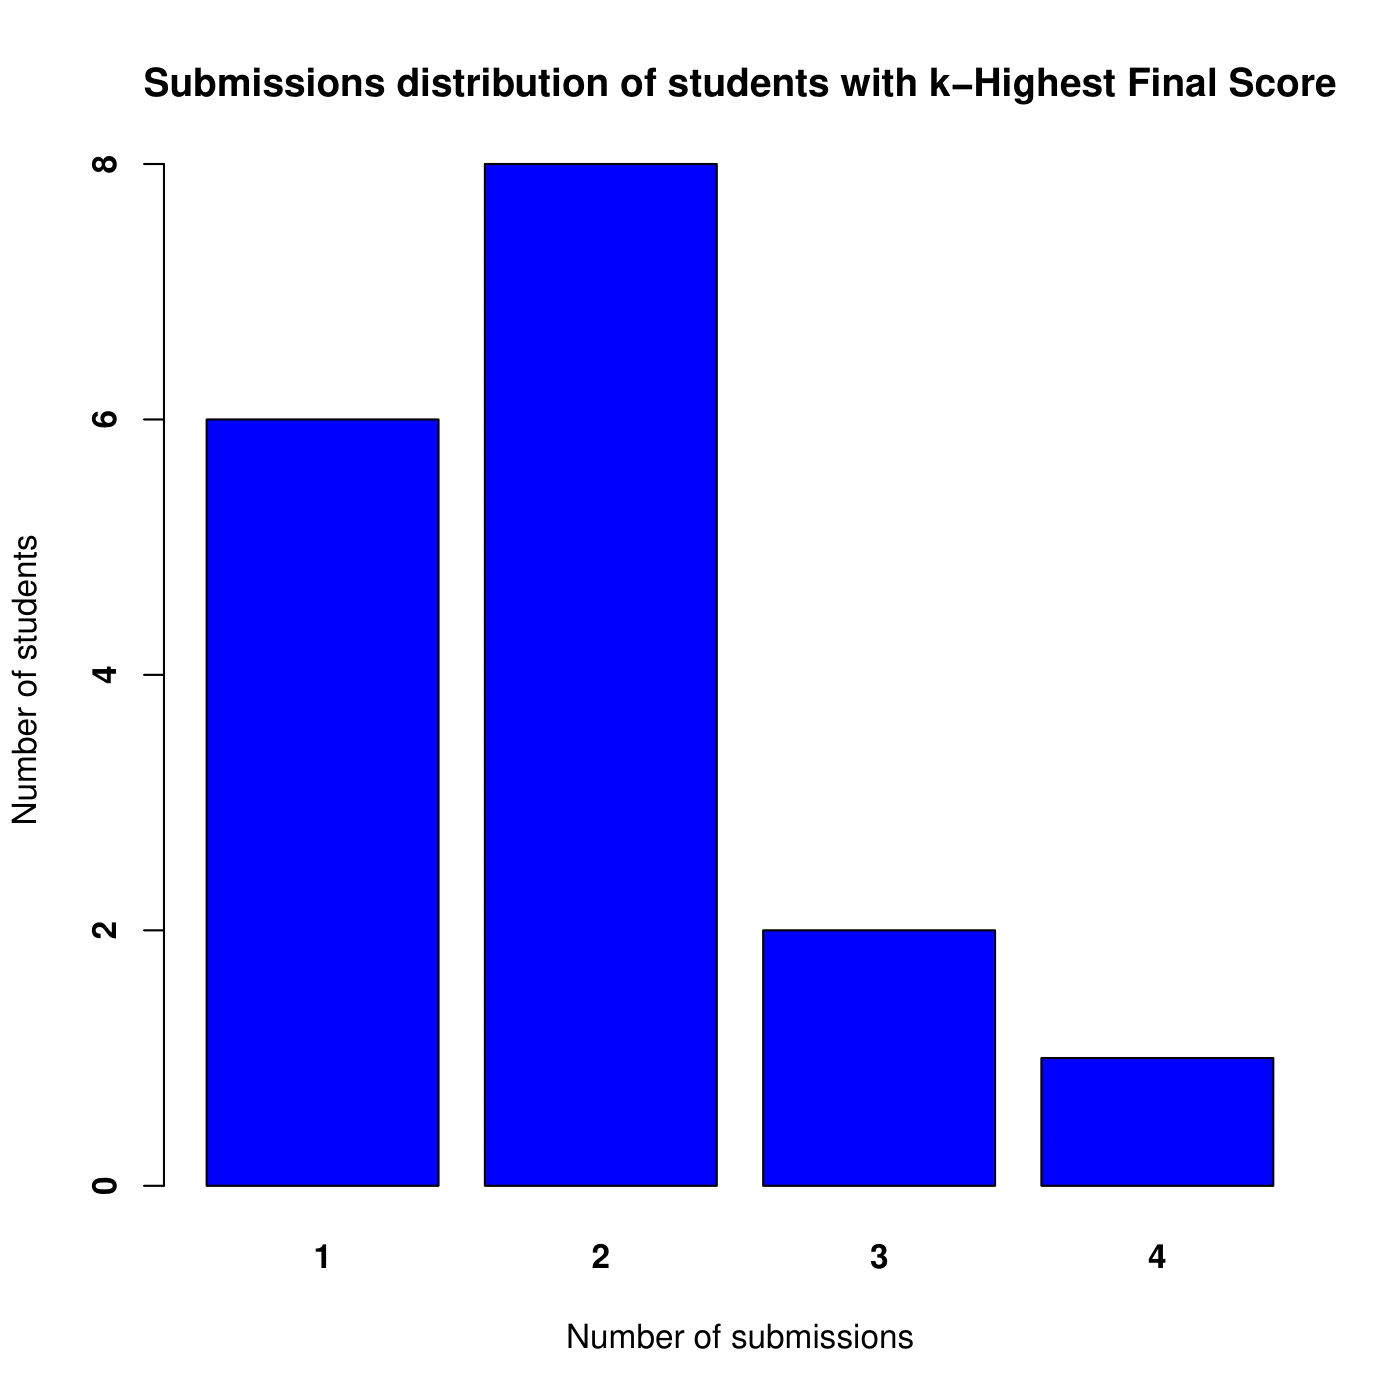
\includegraphics[width = 6 cm]{Images/img2-7-1.png}\\
        Kết quả của quiz 1.4
    \end{center}
\end{itemize}
}

%%%%%%%%%%%%%%%%%%%%%%%%%%%%%%%%%%%%%%%%%%%%%%%%%%%%%%%%%%%%%%%
\subsection{Bài 3}
\frame
{
\frametitle{Nhóm câu hỏi liên quan đến số lần nộp bài}
\framesubtitle{Xác định số lần nộp bài ít nhất}
\begin{itemize}
    \item Ý tưởng thực hiện: $count(), min()$
    \item Kết quả:\\
    \begin{center}
        \begin{tabular}{l l c c c}
             Quiz 1.4 & $\;$ & 1 lần\\
             Quiz 1.5 & $\;$ & 1 lần\\
             Quiz 3.3 & $\;$ & 1 lần\\
             Quiz 4.2 & $\;$ & 1 lần
        \end{tabular}
    \end{center}
\end{itemize}
}

\frame
{
\frametitle{Nhóm câu hỏi liên quan đến điểm số sinh viên}
\framesubtitle{Xác định phổ điểm các sinh viên có số lần nộp bài ít nhất}
\begin{itemize}
    \item Ý tưởng thực hiện: $barplot()$
    \item Kết quả:\\
    \begin{center}
        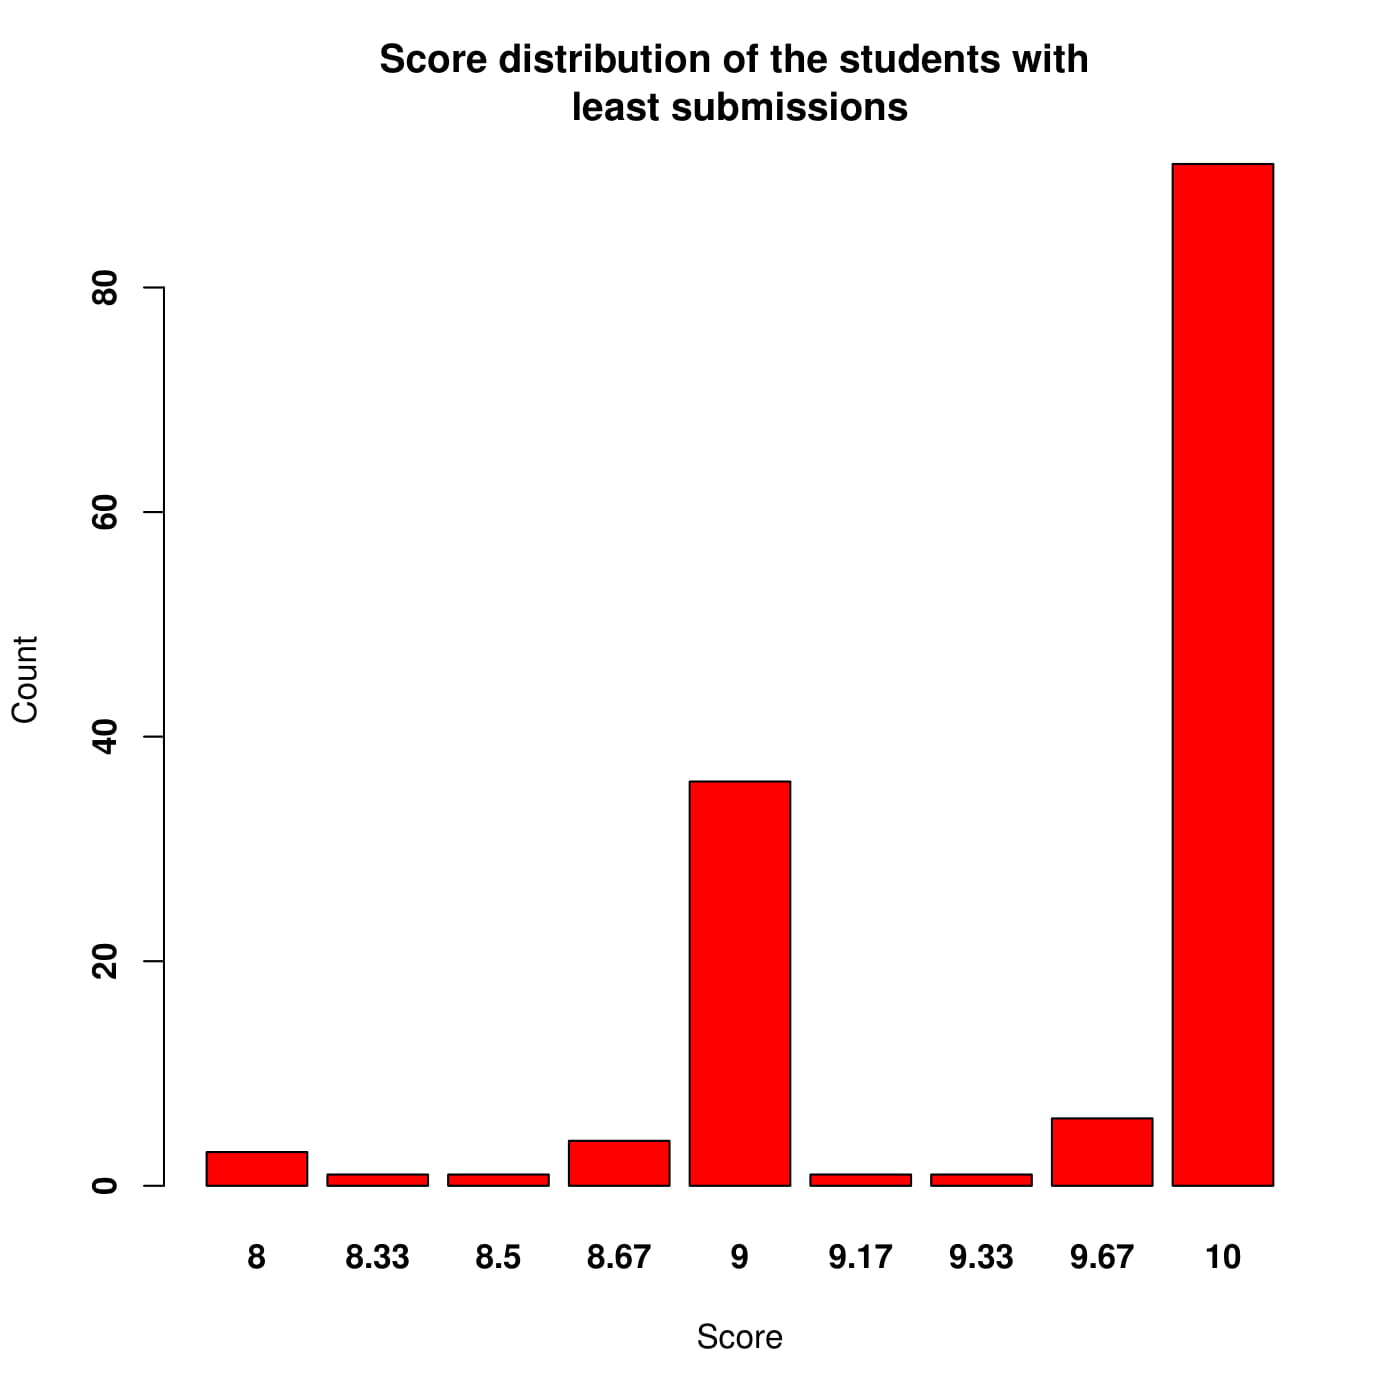
\includegraphics[width = 6 cm]{Images/img3-1-1.jpg}\\
        Kết quả của quiz 1.4
    \end{center}
\end{itemize}
}

\frame
{
\frametitle{Nhóm câu hỏi liên quan đến số lần nộp bài}
\framesubtitle{Xác định số lần nộp bài nhiều nhất}
\begin{itemize}
    \item Ý tưởng thực hiện: $count(), max()$
    \item Kết quả:\\
    \begin{center}
        \begin{tabular}{l l c c c}
             Quiz 1.4 & $\;$ & 5 lần\\
             Quiz 1.5 & $\;$ & 5 lần\\
             Quiz 3.3 & $\;$ & 3 lần\\
             Quiz 4.2 & $\;$ & 3 lần
        \end{tabular}
    \end{center}
\end{itemize}
}

\frame
{
\frametitle{Nhóm câu hỏi liên quan đến điểm số sinh viên}
\framesubtitle{Xác định phổ điểm của các sinh viên có số lần nộp bài nhiều nhất}
\begin{itemize}
    \item Ý tưởng thực hiện: $barplot()$
    \item Kết quả:\\
    \begin{center}
        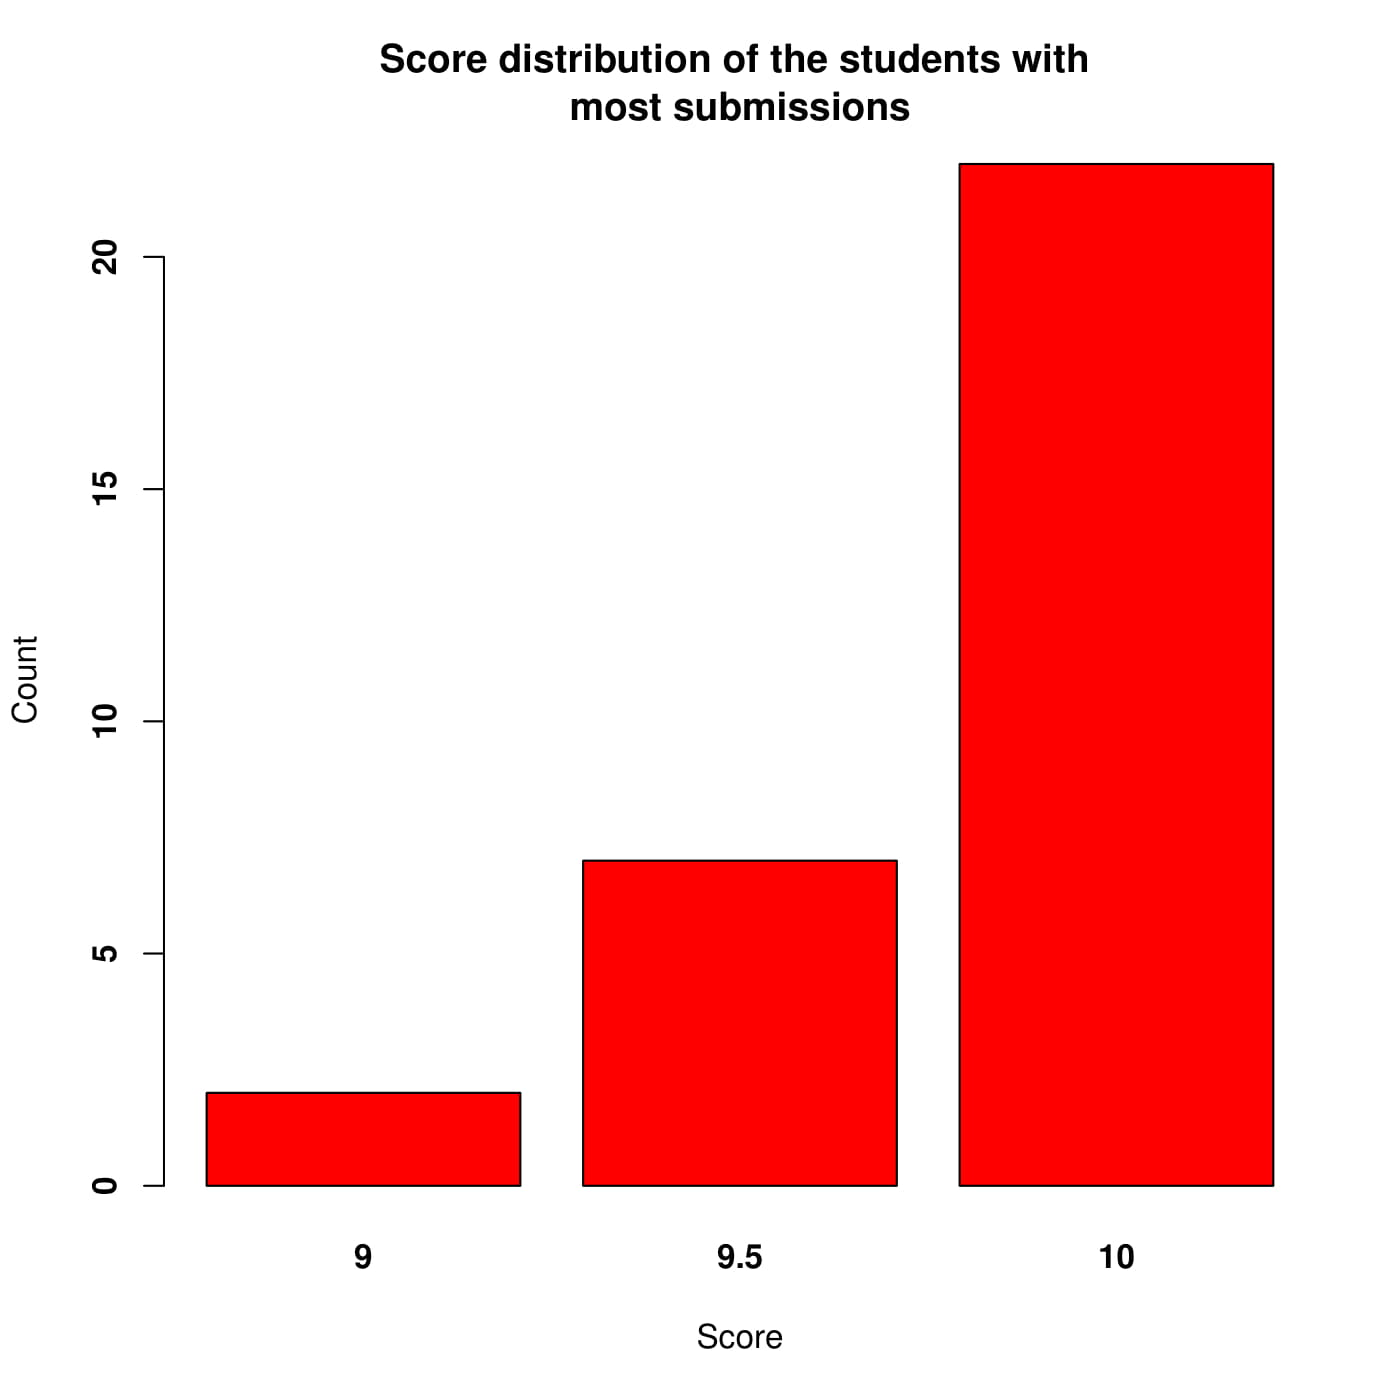
\includegraphics[width = 6 cm]{Images/img3-2-4.png}\\
        Kết quả của quiz 4.2
    \end{center}
\end{itemize}
}

\frame
{
\frametitle{Nhóm câu hỏi liên quan đến số lần nộp bài}
\framesubtitle{Xác định số lần nộp bài trung bình}
\begin{itemize}
    \item Ý tưởng thực hiện: $avg(), round()$
    \item Kết quả:\\
    \begin{center}
        \begin{tabular}{l l c c c}
             Quiz 1.4 & $\;$ & 2 lần\\
             Quiz 1.5 & $\;$ & 2 lần\\
             Quiz 3.3 & $\;$ & 1 lần\\
             Quiz 4.2 & $\;$ & 2 lần
        \end{tabular}
    \end{center}
\end{itemize}
}

\frame
{
\frametitle{Nhóm câu hỏi liên quan đến số lần nộp bài}
\framesubtitle{Xác định số lượng sinh viên có số lần nộp bài trung bình}
\begin{itemize}
    \item Ý tưởng thực hiện: $subset(), length()$
    \item Kết quả:\\
    \begin{center}
        \begin{tabular}{l l c c c}
             Quiz 1.4 & $\;$ & 160 sinh viên\\
             Quiz 1.5 & $\;$ & 163 sinh viên\\
             Quiz 3.3 & $\;$ & 210 sinh viên\\
             Quiz 4.2 & $\;$ & 175 sinh viên
        \end{tabular}
    \end{center}
\end{itemize}
}

\frame
{
\frametitle{Nhóm câu hỏi liên quan đến điểm số sinh viên}
\framesubtitle{Xác định phổ theo điểm số của các sinh viên có lần nộp bài trung bình}
\begin{itemize}
    \item Ý tưởng thực hiện: $barplot()$
    \item Kết quả:\\
    \begin{center}
        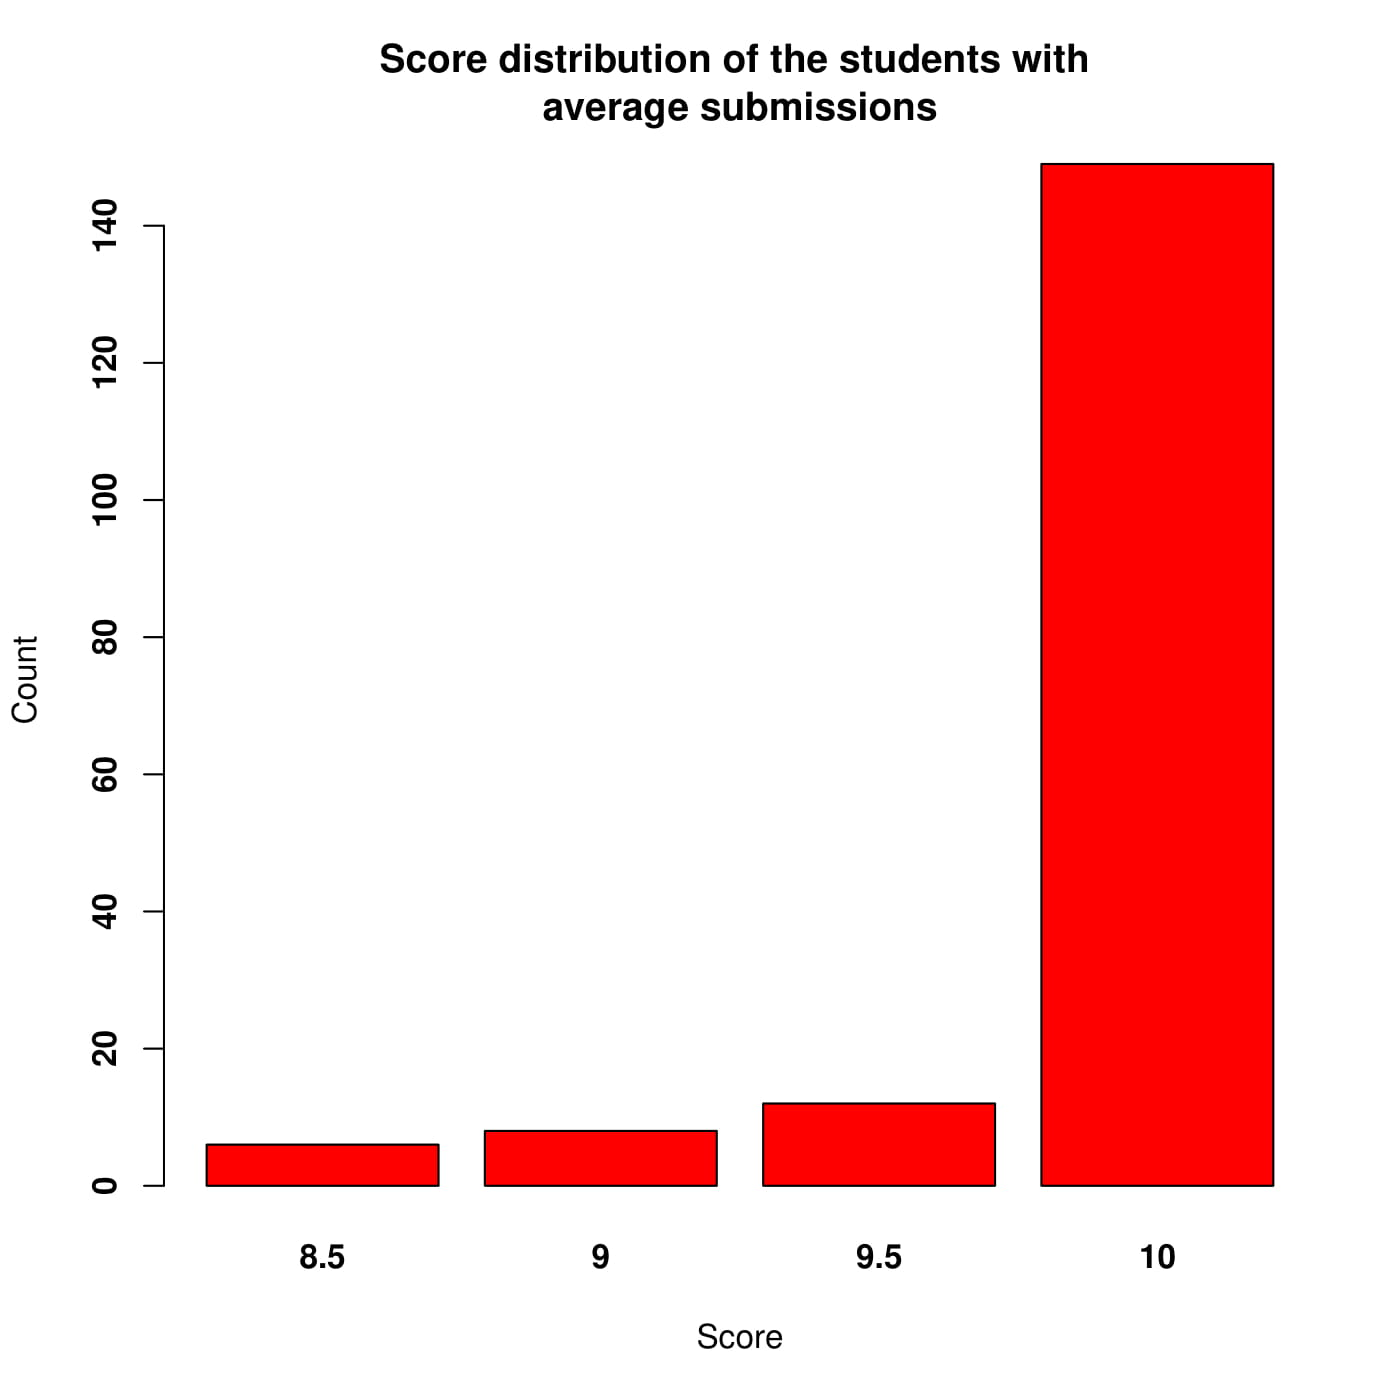
\includegraphics[width = 6 cm]{Images/img3-3-4.png}\\
        Kết quả của quiz 4.2
    \end{center}
\end{itemize}
}

\frame
{
\frametitle{Nhóm câu hỏi liên quan đến số lần nộp bài}
\framesubtitle{Tính trung vị, cực đại, cực tiểu}
\begin{itemize}
    \item Ý tưởng thực hiện: $median(), max(), min()$
    \item Kết quả:\\
    \begin{center}
        \begin{tabular}{l l c c c}
             & & Trung vị & Cực đại & Cực tiểu\\
             Quiz 1.4 & $\;$ & 10 & 10 & 8\\
             Quiz 1.5 & $\;$ & 10 & 10 & 7\\
             Quiz 3.3 & $\;$ & 10 & 10 & 8\\
             Quiz 4.2 & $\;$ & 10 & 10 & 8.5
        \end{tabular}
    \end{center}
\end{itemize}
}

\frame
{
\frametitle{Nhóm câu hỏi liên quan đến số lần nộp bài}
\framesubtitle{Đo mức độ phân tán của mẫu xung quanh giá trị trung bình}
\begin{itemize}
    \item Ý tưởng thực hiện: $var(), sd()$
    \item Kết quả:\\
    \begin{center}
        \begin{tabular}{l l c c c}
             & & Phương sai & Độ lệch chuẩn\\
             Quiz 1.4 & $\;$ & 0.07158138 & 0.267547\\
             Quiz 1.5 & $\;$ & 0.114936 & 0.3390221\\
             Quiz 3.3 & $\;$ & 0.1229437 & 0.3506333\\
             Quiz 4.2 & $\;$ & 0.1234319 & 0.3513287
        \end{tabular}
    \end{center}
\end{itemize}
}

\frame
{
\frametitle{Nhóm câu hỏi liên quan đến số lần nộp bài}
\framesubtitle{Tính độ méo lệch, độ nhọn}
\begin{itemize}
    \item Ý tưởng thực hiện: $skewness(), kurtosis()$
    \item Kết quả:\\
    \begin{center}
        \begin{tabular}{l l c c c}
             & & Độ méo lệch & Độ nhọn\\
             Quiz 1.4 & $\;$ & -5.477856 & 6.59856\\
             Quiz 1.5 & $\;$ & -5.241093 & 37.8015\\
             Quiz 3.3 & $\;$ & -3.524972 & 5.58703\\
             Quiz 4.2 & $\;$ & -2.775748 & 9.813872
        \end{tabular}
    \end{center}
\end{itemize}
}

\frame
{
\frametitle{Nhóm câu hỏi liên quan đến số lần nộp bài}
\framesubtitle{Tính tứ phân vị thứ nhất - thứ ba}
\begin{itemize}
    \item Ý tưởng thực hiện: $quantile()$
    \item Kết quả:\\
    \begin{center}
        \begin{tabular}{l l c c c}
             & & Thứ nhất & Thứ ba\\
             Quiz 1.4 & $\;$ & 10 & 10\\
             Quiz 1.5 & $\;$ & 10 & 10\\
             Quiz 3.3 & $\;$ & 10 & 10\\
             Quiz 4.2 & $\;$ & 10 & 10
        \end{tabular}
    \end{center}
\end{itemize}
}

\frame
{
\frametitle{Nhóm câu hỏi liên quan đến số lần nộp bài}
\framesubtitle{Xác định số lượng sinh viên nằm trong nhóm có số lần nộp bài nhiều nhất hoặc nhiều nhì}
\begin{itemize}
    \item Ý tưởng thực hiện: $length()$
    \item Kết quả:\\
    \begin{center}
        \begin{tabular}{l l c c c}
             Quiz 1.4 & $\;$ & 8 sinh viên\\
             Quiz 1.5 & $\;$ & 7 sinh viên\\
             Quiz 3.3 & $\;$ & 70 sinh viên\\
             Quiz 4.2 & $\;$ & 206 sinh viên
        \end{tabular}
    \end{center}
\end{itemize}
}

\frame
{
\frametitle{Nhóm câu hỏi liên quan đến điểm số sinh viên}
\framesubtitle{Xác định phổ theo điểm số của các sinh viên có lần nộp bài nhiều nhất hoặc nhiều nhì}
\begin{itemize}
    \item Ý tưởng thực hiện: $barplot()$
    \item Kết quả:\\
    \begin{center}
        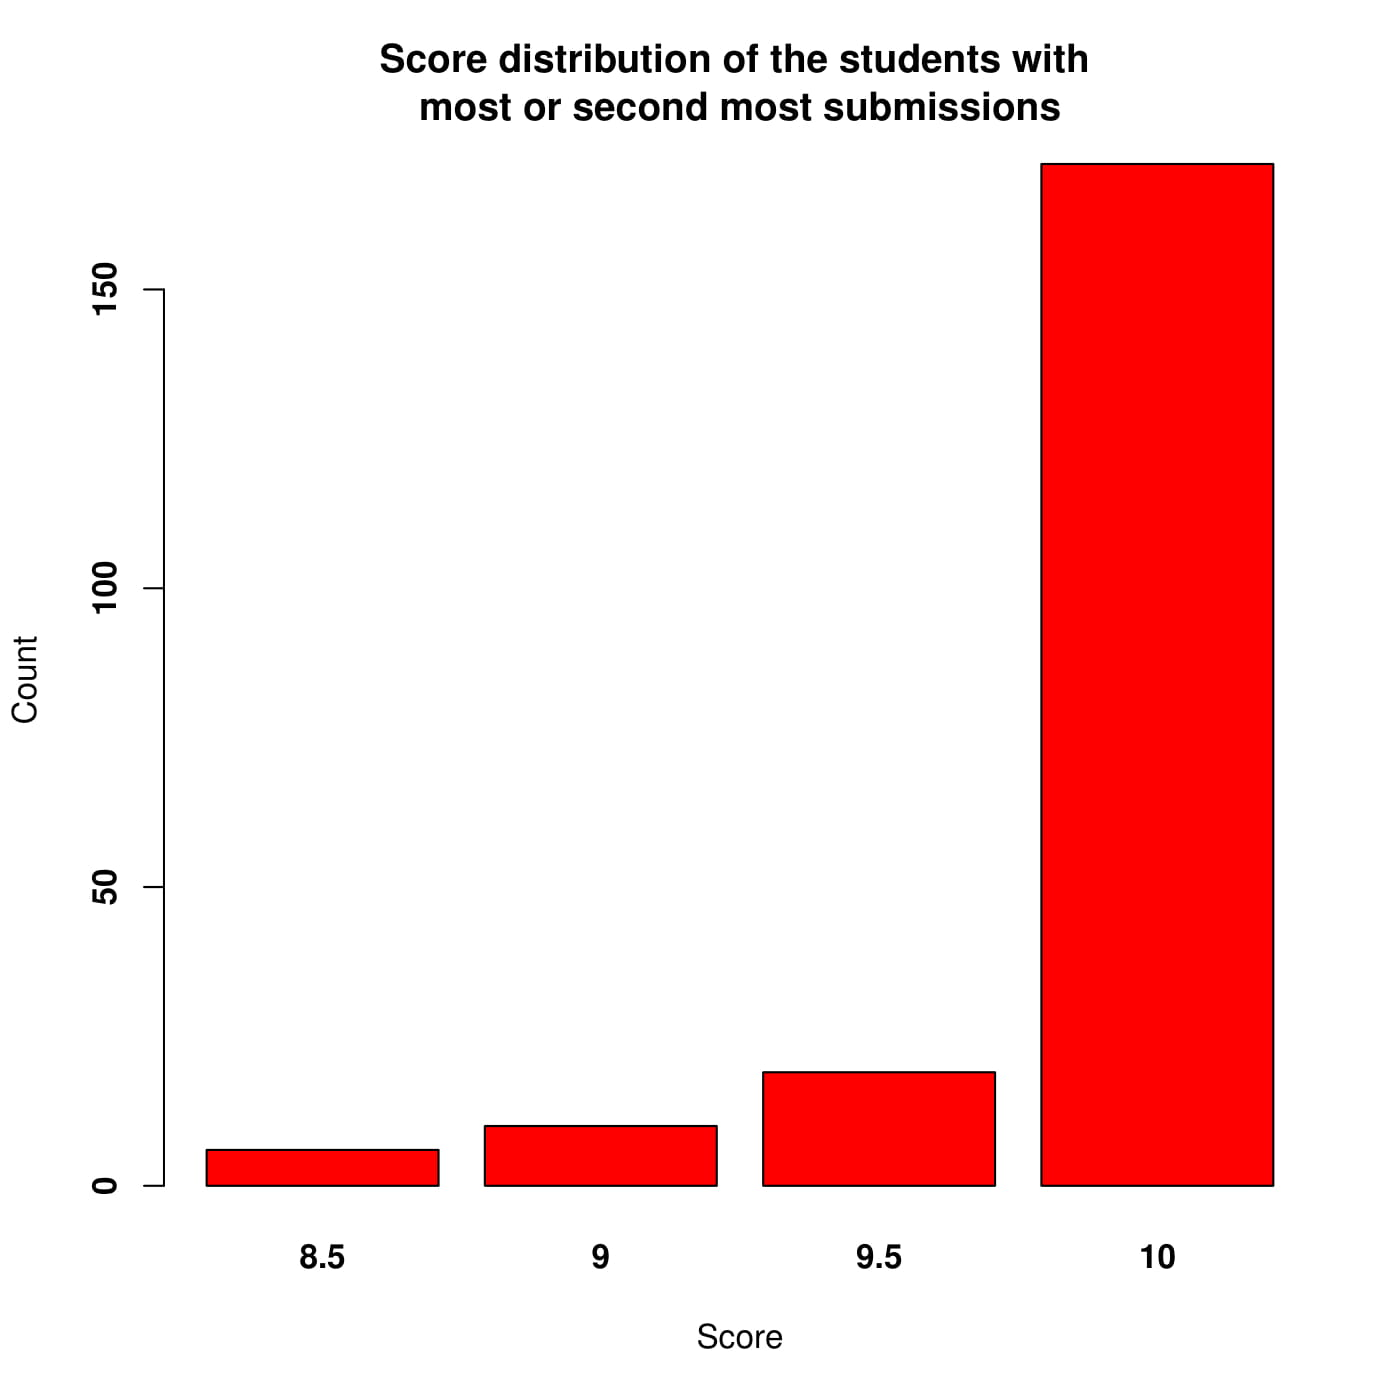
\includegraphics[width = 6 cm]{Images/img3-4-4.png}\\
        Kết quả của quiz 4.2
    \end{center}
\end{itemize}
}

\frame
{
\frametitle{Nhóm câu hỏi liên quan đến số lần nộp bài}
\framesubtitle{Xác định số lượng các sinh viên nằm trong nhóm một phần ba đầu theo thứ tự số lần nộp bài giảm dần}
\begin{itemize}
    \item Ý tưởng thực hiện: $head(), order(), length()$
    \item Kết quả:\\
    \begin{center}
        \begin{tabular}{l l c c c}
             Quiz 1.4 & $\;$ & 114 sinh viên\\
             Quiz 1.5 & $\;$ & 114 sinh viên\\
             Quiz 3.3 & $\;$ & 93 sinh viên\\
             Quiz 4.2 & $\;$ & 86 sinh viên
        \end{tabular}
    \end{center}
\end{itemize}
}

\frame
{
\frametitle{Nhóm câu hỏi liên quan đến điểm số sinh viên}
\framesubtitle{Xác định phổ theo điểm số của các sinh viên nằm trong nhóm một phần ba đầu theo thứ tự số lần nộp bài giảm dần}
\begin{itemize}
    \item Ý tưởng thực hiện: $barplot()$
    \item Kết quả:\\
    \begin{center}
        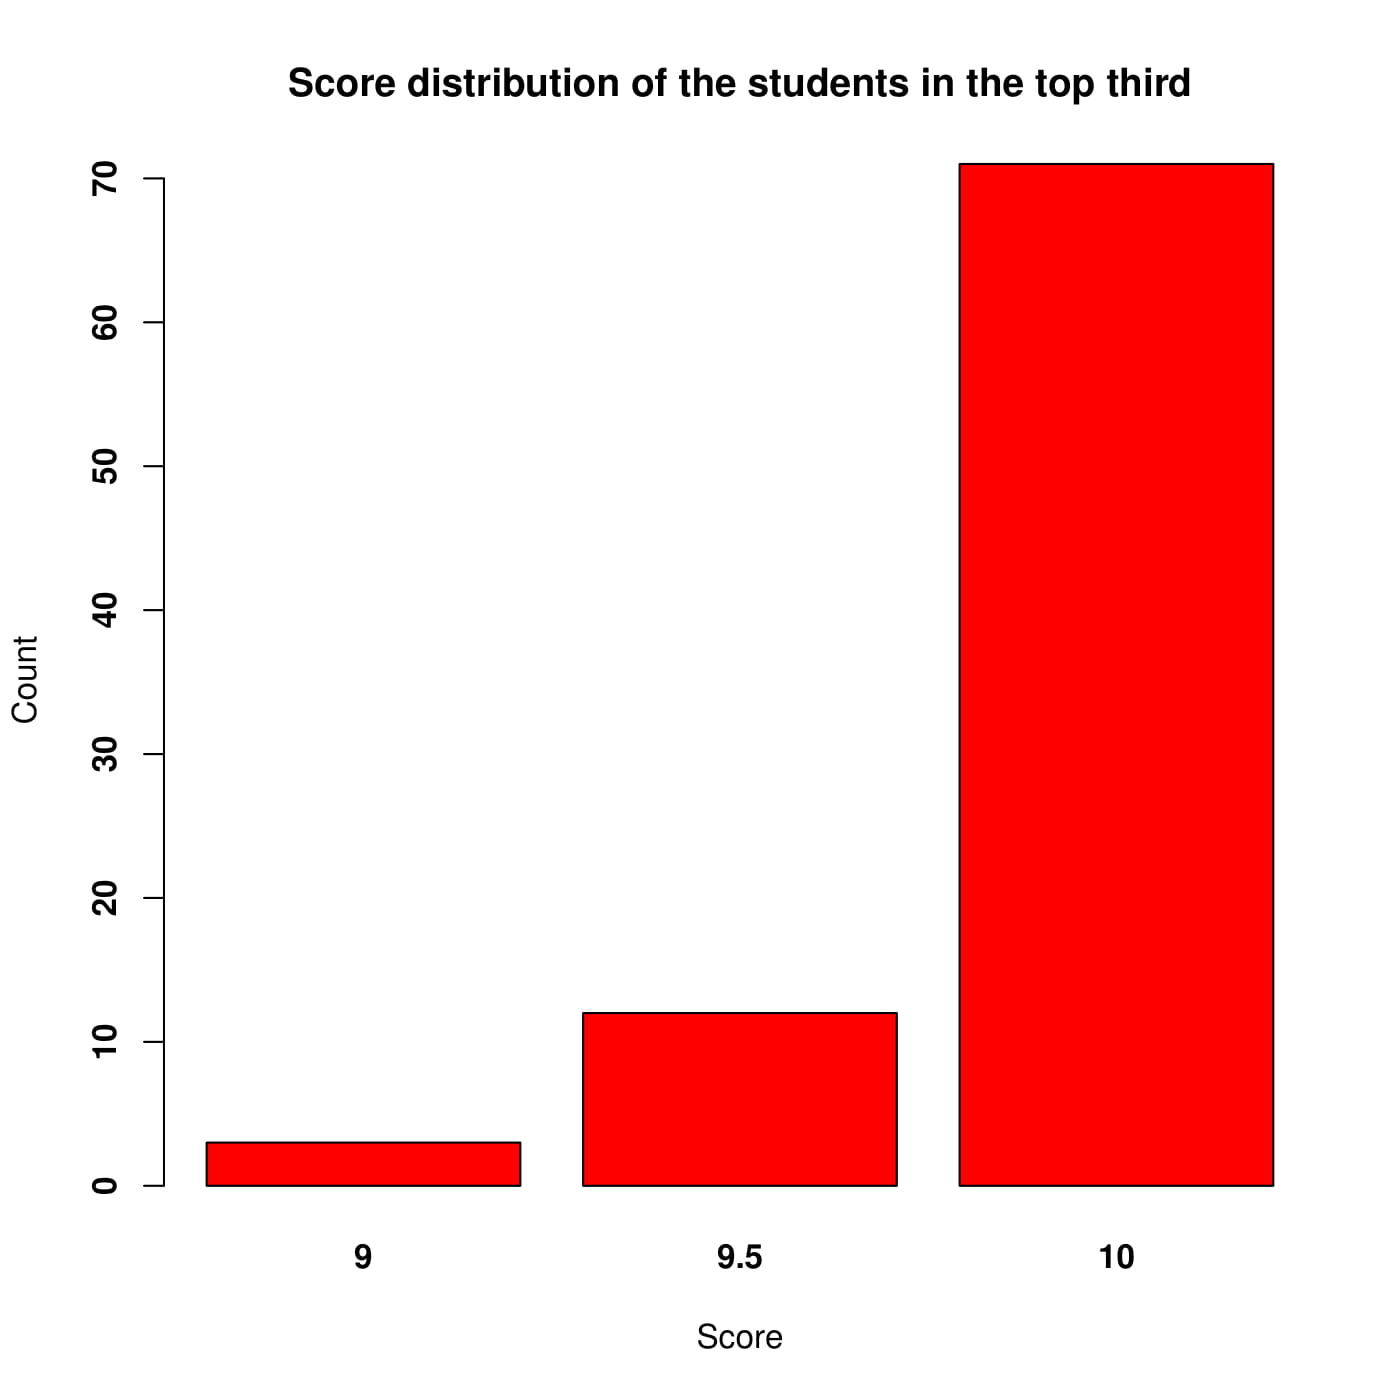
\includegraphics[width = 6 cm]{Images/img3-5-4.png}\\
        Kết quả của quiz 4.2
    \end{center}
\end{itemize}
}

\frame
{
\frametitle{Nhóm câu hỏi liên quan đến điểm số sinh viên}
\framesubtitle{Xác định phổ theo điểm số của các sinh viên nằm trong k nhóm đầu xếp theo số lần nộp bài giảm dần}
\begin{itemize}
    \item Ý tưởng thực hiện: $subset(), barplot()$
    \item Kết quả: giả sử k = 2\\
    \begin{center}
        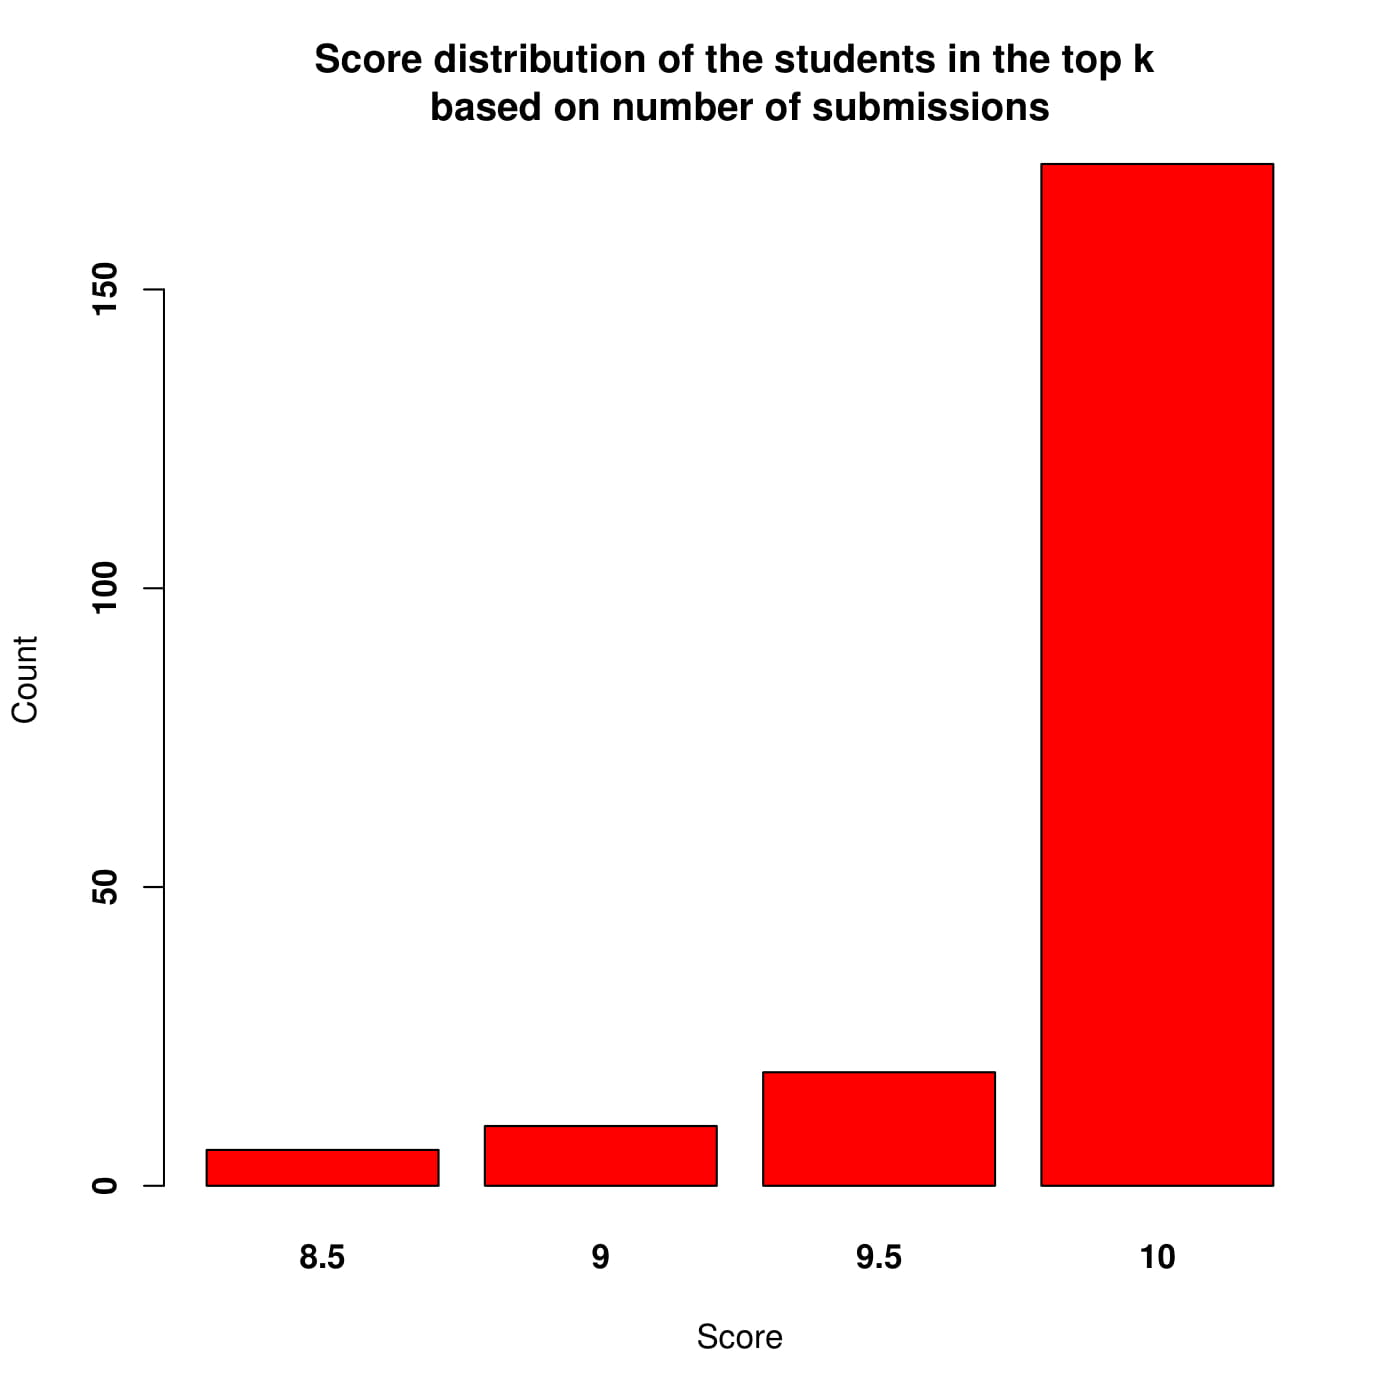
\includegraphics[width = 6 cm]{Images/img3-6-4.png}\\
        Kết quả của quiz 4.2
    \end{center}
\end{itemize}
}

%%%%%%%%%%%%%%%%%%%%%%%%%%%%%%%%%%%%%%%%%%%%%%%%%%%%%%%%%%%%%%%%%%%%%%%%
\subsection{Bài 4}
\frame
{
\frametitle{Nhóm câu hỏi liên quan đến thời gian, tần suất nộp bài của các sinh viên}
\framesubtitle{Xác định thời gian dài nhất tính từ lần nộp bài đầu tiên đến lần nộp cuối}
\begin{itemize}
    \item Ý tưởng thực hiện: $max()$
    \item Kết quả:\\
    \begin{center}
        \begin{tabular}{l l c c c}
             Quiz 1.4 & $\;$ & 73468 phút\\
             Quiz 1.5 & $\;$ & 67413 phút\\
             Quiz 3.3 & $\;$ & 32769 phút\\
             Quiz 4.2 & $\;$ & 30862 phút
        \end{tabular}
    \end{center}
\end{itemize}
}

\frame
{
\frametitle{Nhóm câu hỏi liên quan đến thời gian, tần suất nộp bài của các sinh viên}
\framesubtitle{Xác định phổ thời gian làm việc của các sinh viên}
\begin{itemize}
    \item Ý tưởng thực hiện: $hist()$
    \item Kết quả:\\
    \begin{center}
        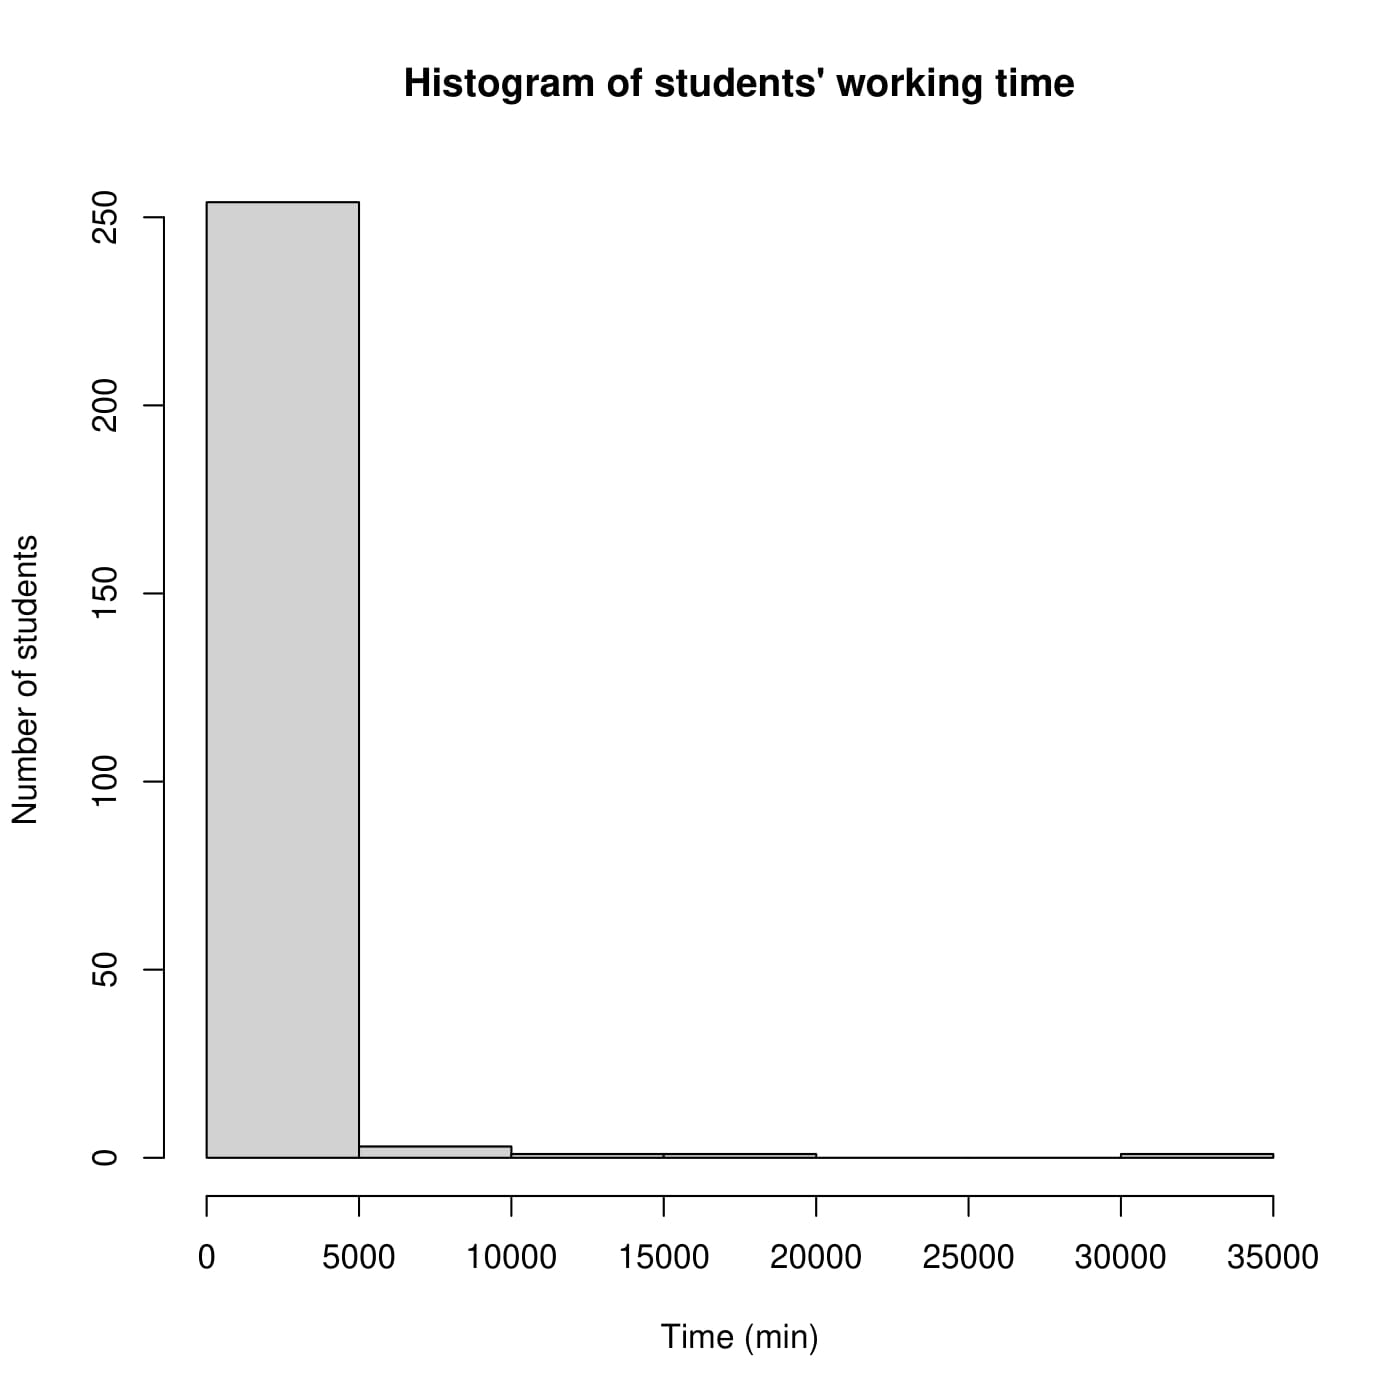
\includegraphics[width = 6 cm]{Images/img4-1-4.png}\\
        Kết quả của quiz 4.2
    \end{center}
\end{itemize}
}

\frame
{
\frametitle{Nhóm câu hỏi liên quan đến thời gian, tần suất nộp bài của các sinh viên}
\framesubtitle{Xác định phổ điểm của các sinh viên có tần suất nộp bài ít nhất}
\begin{itemize}
    \item Ý tưởng thực hiện: $hist(), subset(), unique(), match()$
    \item Kết quả:\\
    \begin{center}
        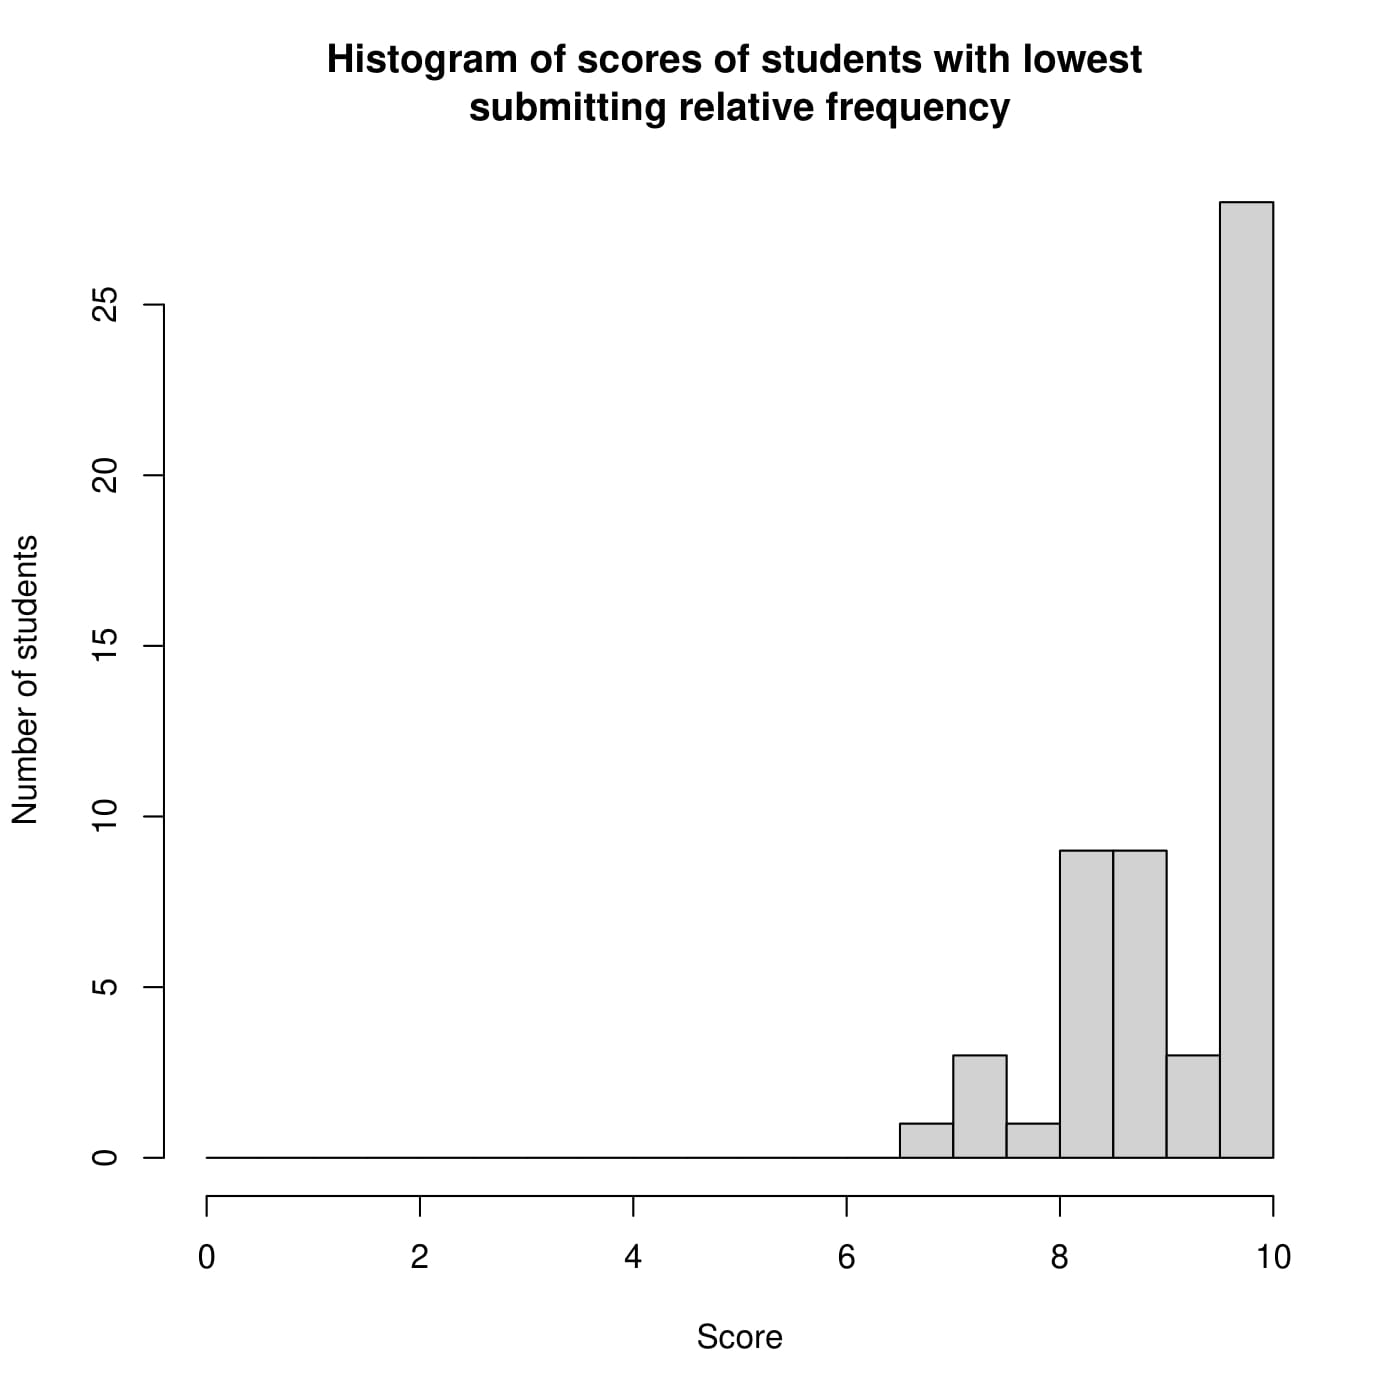
\includegraphics[width = 6 cm]{Images/img4-2-4.png}\\
        Kết quả của quiz 4.2
    \end{center}
\end{itemize}
}

\frame
{
\frametitle{Nhóm câu hỏi liên quan đến thời gian, tần suất nộp bài của các sinh viên}
\framesubtitle{Xác định số lượng sinh viên có tần suất nộp bài nhiều nhất}
\begin{itemize}
    \item Ý tưởng thực hiện: $subset()$
    \item Kết quả:\\
    \begin{center}
        \begin{tabular}{l l c c c}
             Quiz 1.4 & $\;$ & 1 sinh viên\\
             Quiz 1.5 & $\;$ & 1 sinh viên\\
             Quiz 3.3 & $\;$ & 1 sinh viên\\
             Quiz 4.2 & $\;$ & 1 sinh viên
        \end{tabular}
    \end{center}
\end{itemize}
}

\frame
{
\frametitle{Nhóm câu hỏi liên quan đến thời gian, tần suất nộp bài của các sinh viên}
\framesubtitle{Xác định phổ điểm của các sinh viên có tần suất nộp bài nhiều nhất}
\begin{itemize}
    \item Ý tưởng thực hiện: $hist()$
    \item Kết quả:\\
    \begin{center}
        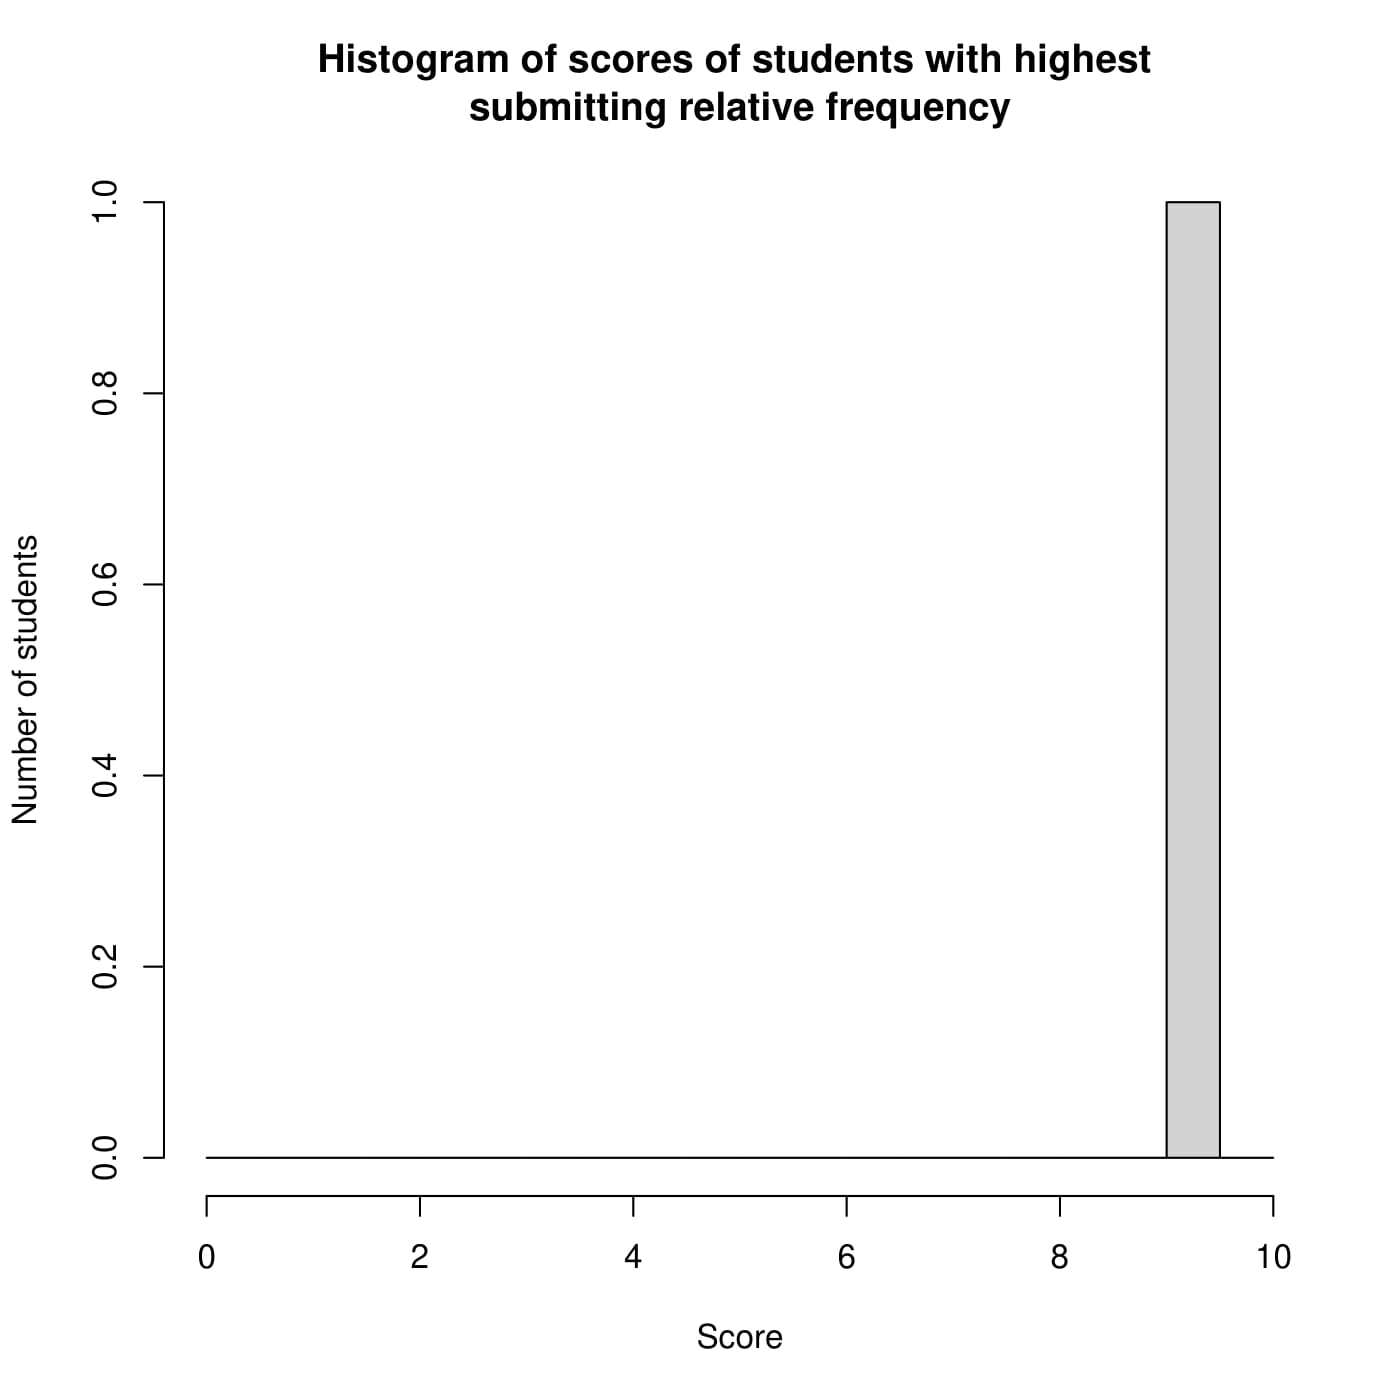
\includegraphics[width = 6 cm]{Images/img4-3-4.png}\\
        Kết quả của quiz 4.2
    \end{center}
\end{itemize}
}

\frame
{
\frametitle{Nhóm câu hỏi liên quan đến thời gian, tần suất nộp bài của các sinh viên}
\framesubtitle{Vẽ biểu đồ tần số của mẫu trên}
\begin{itemize}
    \item Ý tưởng thực hiện: $table(), barplot()$
    \item Kết quả:\\
    \begin{center}
        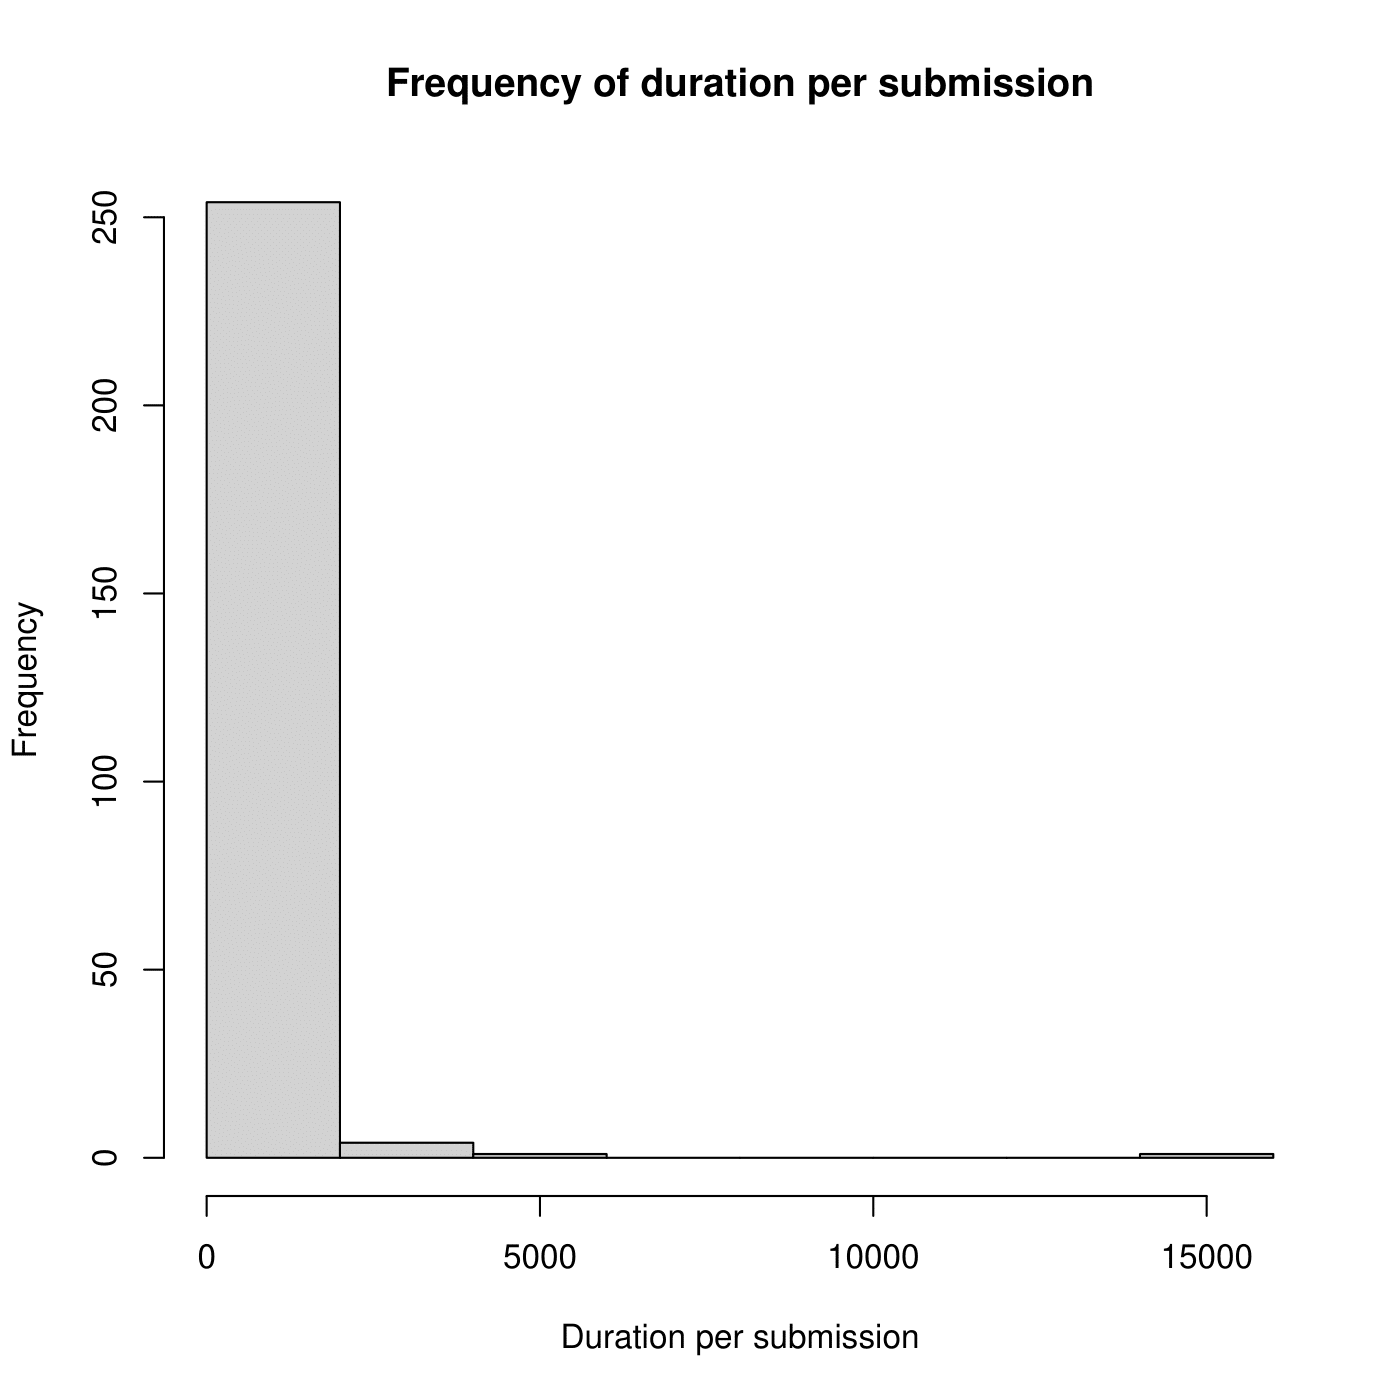
\includegraphics[width = 6 cm]{Images/img4-4-4.png}\\
        Kết quả của quiz 4.2
    \end{center}
\end{itemize}
}

\frame
{
\frametitle{Nhóm câu hỏi liên quan đến thời gian, tần suất nộp bài của các sinh viên}
\framesubtitle{Vẽ biểu đồ tần suất của mẫu trên}
\begin{itemize}
    \item Ý tưởng thực hiện: $table(), barplot()$
    \item Kết quả:\\
    \begin{center}
        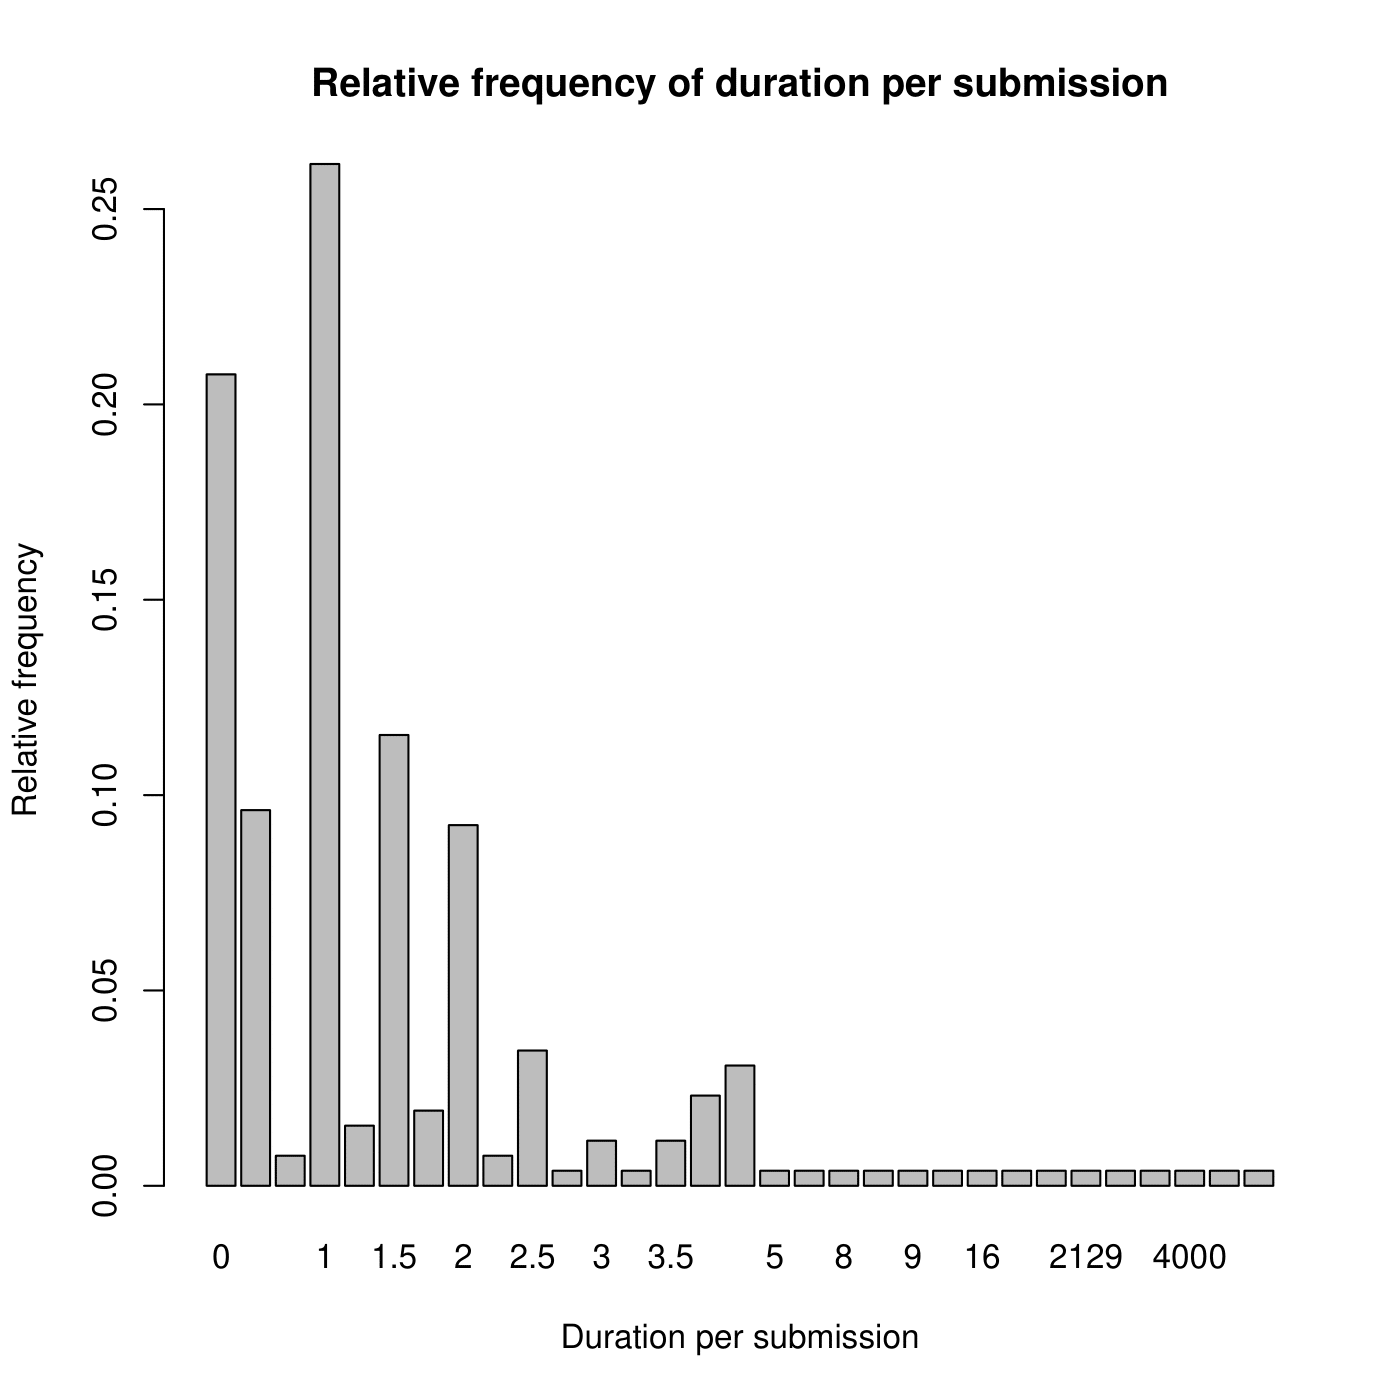
\includegraphics[width = 6 cm]{Images/img4-5-4.png}\\
        Kết quả của quiz 4.2
    \end{center}
\end{itemize}
}

\frame
{
\frametitle{Nhóm câu hỏi liên quan đến thời gian, tần suất nộp bài của các sinh viên}
\framesubtitle{Vẽ biểu đồ tần suất tích lũy của mẫu trên}
\begin{itemize}
    \item Ý tưởng thực hiện: $table(), cumsum(), barplot()$
    \item Kết quả:\\
    \begin{center}
        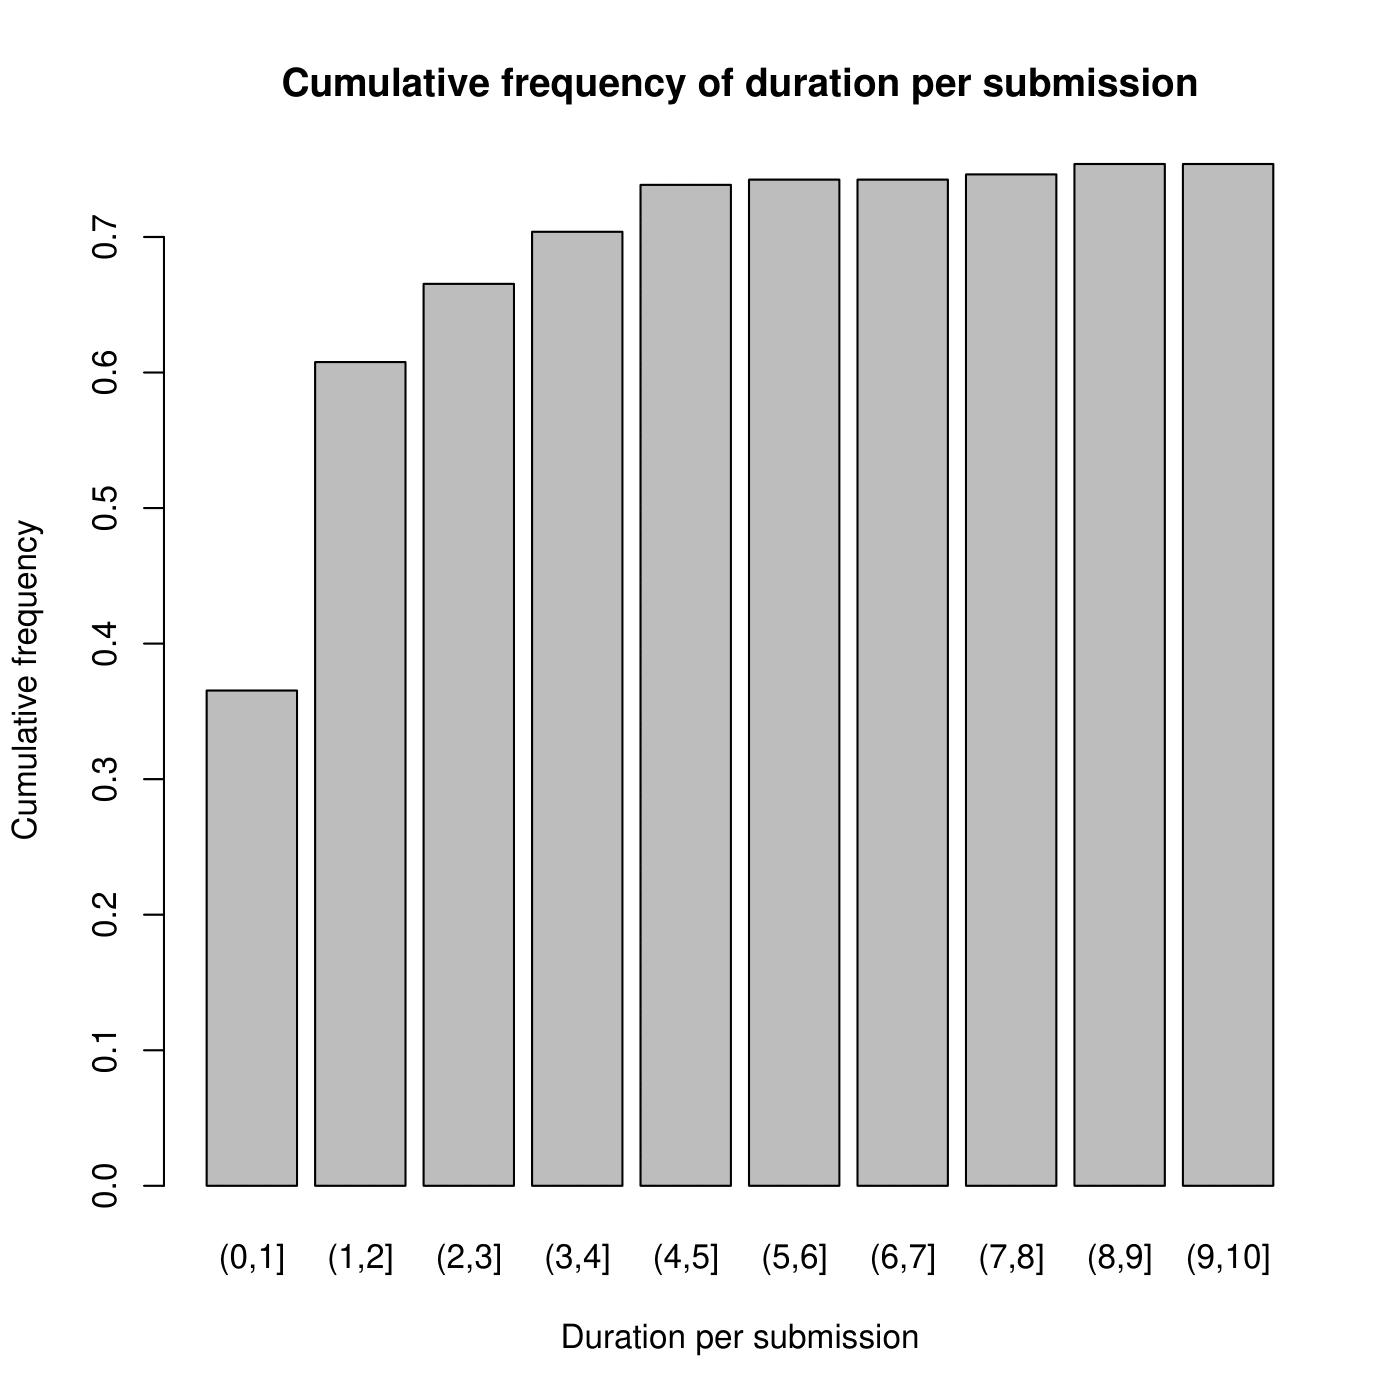
\includegraphics[width = 6 cm]{Images/img4-6-4.png}\\
        Kết quả của quiz 4.2
    \end{center}
\end{itemize}
}

\frame
{
\frametitle{Nhóm câu hỏi liên quan đến thời gian, tần suất nộp bài của các sinh viên}
\framesubtitle{Tính trung vị mẫu, cực đại mẫu, cực tiểu mẫu của trên}
\begin{itemize}
    \item Ý tưởng thực hiện: $subset(), median(), min(), max()$
    \item Kết quả:\\
    \begin{center}
        \begin{tabular}{l l c c c}
             & & Trung vị & Cực đại & Cực tiểu\\
             Quiz 1.4 & $\;$ & 0.5 & 28791 & 0\\
             Quiz 1.5 & $\;$ & 1 & 33706.5 & 0\\
             Quiz 3.3 & $\;$ & 0 & 12740.5 & 0\\
             Quiz 4.2 & $\;$ & 1 & 15431 & 0
        \end{tabular}
    \end{center}
\end{itemize}
}

\frame
{
\frametitle{Nhóm câu hỏi liên quan đến thời gian, tần suất nộp bài của các sinh viên}
\framesubtitle{Đo mức độ phân tán của mẫu}
\begin{itemize}
    \item Ý tưởng thực hiện: $var(), sd()$
    \item Kết quả:\\
    \begin{center}
        \begin{tabular}{l l c c c}
             & & Phương sai & Độ lệch chuẩn\\
             Quiz 1.4 & $\;$ & 9202857 & 3033.621\\
             Quiz 1.5 & $\;$ & 14189912 & 3766.95\\
             Quiz 3.3 & $\;$ & 1109978 & 1053.555\\
             Quiz 4.2 & $\;$ & 1175476 & 1084.194
        \end{tabular}
    \end{center}
\end{itemize}
}

\frame
{
\frametitle{Nhóm câu hỏi liên quan đến thời gian, tần suất nộp bài của các sinh viên}
\framesubtitle{Tính độ méo lệch, độ nhọn}
\begin{itemize}
    \item Ý tưởng thực hiện: $skewness(), kurtosis()$
    \item Kết quả:\\
    \begin{center}
        \begin{tabular}{l l c c c}
             & & Độ méo lệch & Độ nhọn\\
             Quiz 1.4 & $\;$ & 6.28353 & 46.24756\\
             Quiz 1.5 & $\;$ & 5.845597 & 39.97973\\
             Quiz 3.3 & $\;$ & 10.48039 & 116.0303\\
             Quiz 4.2 & $\;$ & 11.65296 & 156.6423
        \end{tabular}
    \end{center}
\end{itemize}
}

\frame
{
\frametitle{Nhóm câu hỏi liên quan đến thời gian, tần suất nộp bài của các sinh viên}
\framesubtitle{Tính tứ phân vị thứ nhất và thứ ba}
\begin{itemize}
    \item Ý tưởng thực hiện: $quantile()$
    \item Kết quả:\\
    \begin{center}
        \begin{tabular}{l l c c c}
             & & Thứ nhất & Thứ ba\\
             Quiz 1.4 & $\;$ & 0 & 1.5\\
             Quiz 1.5 & $\;$ & 0 & 2\\
             Quiz 3.3 & $\;$ & 0 & 0\\
             Quiz 4.2 & $\;$ & 0.5 & 2
        \end{tabular}
    \end{center}
\end{itemize}
}

%%%%%%%%%%%%%%%%%%%%%%%%%%%%%%%%%%%%%%%%%%%%%%%%%%%%%%
%%%% Bài 5
\subsection{Bài 5}

\frame
{
\frametitle{Nhóm câu hỏi liên quan đến điểm trung bình}
\framesubtitle{Vẽ biểu đồ sự phân bố về điểm đạt được của sinh viên sau k = 6 lần nộp bài}
\begin{itemize}
    \item Ý tưởng thực hiện: $order(), cbind(), match(), hist()$
    \item Kết quả:\\
    \begin{center}
        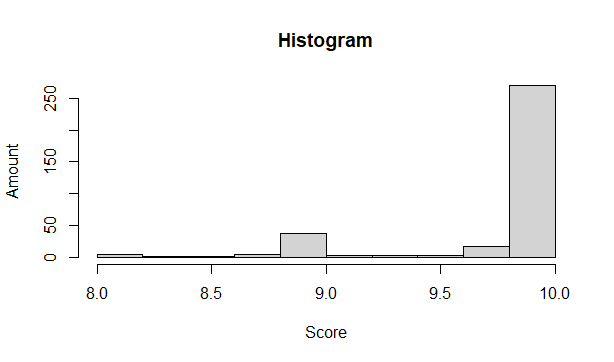
\includegraphics[width = 6 cm]{Images/img5-1-1.png}\\
        Kết quả của quiz 1.4
    \end{center}
\end{itemize}
}

\frame
{
\frametitle{Nhóm câu hỏi liên quan đến điểm trung bình}
\framesubtitle{Vẽ biểu đồ sự phân bố về điểm đạt được của sinh viên sau k = 1 lần nộp bài}
\begin{itemize}
    \item Ý tưởng thực hiện: $order(), cbind(), match(), hist()$
    \item Kết quả:\\
    \begin{center}
        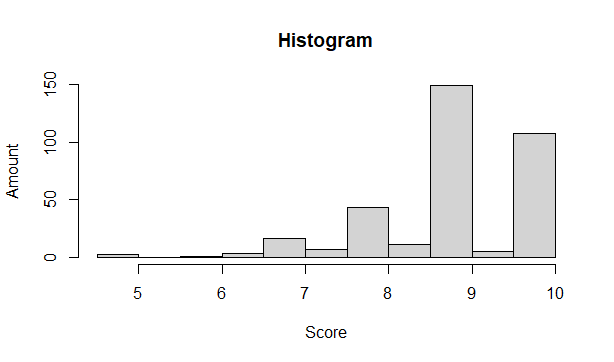
\includegraphics[width = 6 cm]{Images/img5-2-1.png}\\
        Kết quả của quiz 1.4
    \end{center}
\end{itemize}
}

\frame
{
\frametitle{Nhóm câu hỏi liên quan đến điểm trung bình}
\framesubtitle{Vẽ biểu đồ thể hiện sự thay đổi của các giá trị trung bình này với sự thay đổi của k}
\begin{itemize}
    \item Ý tưởng thực hiện: $mean(), cbind(), match()$
    \item Kết quả:\\
    \begin{center}
        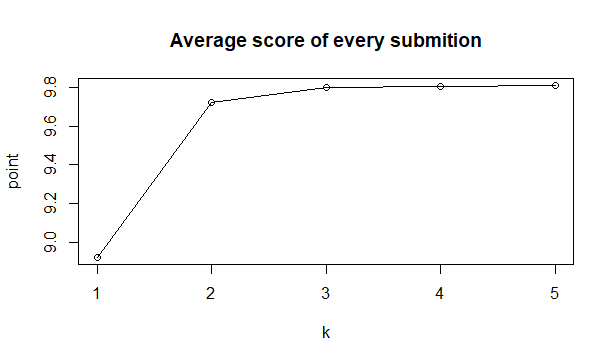
\includegraphics[width = 6 cm]{Images/img5-3-1.png}\\
        Kết quả của quiz 1.4
    \end{center}
\end{itemize}
}

\frame
{
\frametitle{Nhóm câu hỏi liên quan đến điểm trung bình}
\framesubtitle{Tính trung bình điểm số mà các sinh viên đạt được}
\begin{itemize}
    \item Ý tưởng thực hiện: $mean(), cbind(), match()$
    \item Kết quả:\\
    \begin{center}
        \begin{tabular}{l l c c c}
             Quiz 1.4 & $\;$ & 9.81 điểm\\
             Quiz 1.5 & $\;$ & 9.77 điểm\\
             Quiz 3.3 & $\;$ & 9.92 điểm\\
             Quiz 4.2 & $\;$ & 9.76 điểm
        \end{tabular}
    \end{center}
\end{itemize}
}

%%%%%%%%%%%%%%%%%%%%%%%%%%%%%%%%%%%%%%%%%%%%%%%%%%%%%%%%%%%%%%%%%%
%%%%% Bài 7
\subsection{Bài 7}

\frame
{
\frametitle{Nhóm câu hỏi liên quan đến sinh viên học đối phó}
\framesubtitle{Xác định thời điểm $t_2$ phù hợp}
\begin{itemize}
    \item Ý tưởng thực hiện: $order(), match()$
    \item Kết quả:\\
    \begin{center}
        \begin{tabular}{l l c c c}
             Quiz 1.4 & $\;$ & $t_2$ = 12:01 ngày 24/4/2020\\
             Quiz 1.5 & $\;$ & $t_2$ = 18:16 ngày 27/4/2020\\
             Quiz 3.3 & $\;$ & $t_2$ = 19:29 ngày 11/5/2020\\
             Quiz 4.2 & $\;$ & $t_2$ = 20:19 ngày 12/5/2020
        \end{tabular}
    \end{center}
\end{itemize}
}

\frame
{
\frametitle{Nhóm câu hỏi liên quan đến sinh viên học đối phó}
\framesubtitle{Số lượng sinh viên học đối phó}
\begin{itemize}
    \item Ý tưởng thực hiện: $nrow()$
    \item Kết quả:\\
    \begin{center}
        \begin{tabular}{l l c c c}
             Quiz 1.4 & $\;$ & 35 sinh viên\\
             Quiz 1.5 & $\;$ & 35 sinh viên\\
             Quiz 3.3 & $\;$ & 29 sinh viên\\
             Quiz 4.2 & $\;$ & 27 sinh viên
        \end{tabular}
    \end{center}
\end{itemize}
}

\frame
{
\frametitle{Nhóm câu hỏi liên quan đến sinh viên học đối phó}
\framesubtitle{Xác định phổ điểm của các sinh viên học đối phó}
\begin{itemize}
    \item Ý tưởng thực hiện: $hist()$
    \item Kết quả:\\
    \begin{center}
        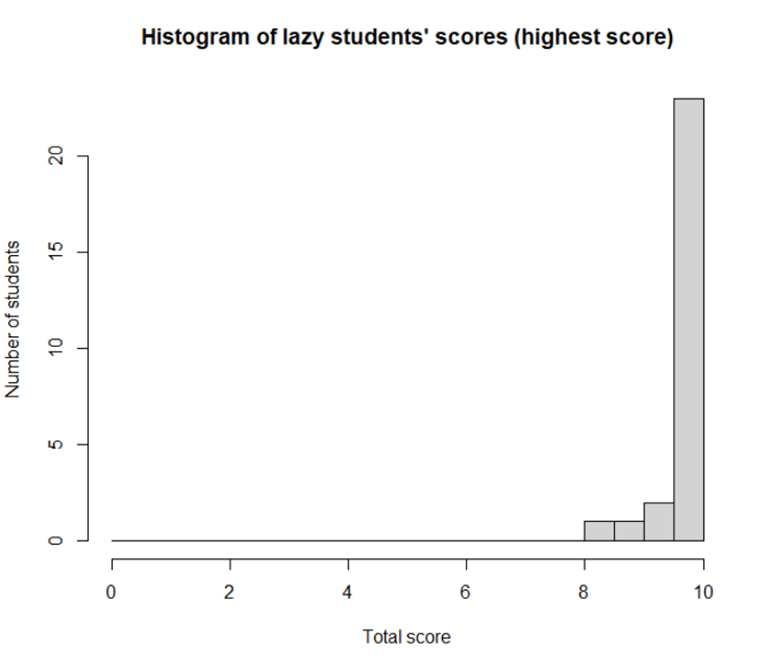
\includegraphics[width = 6 cm]{Images/img7-2-4.png}\\
        Kết quả của quiz 4.2 (điểm tổng kết)
    \end{center}
\end{itemize}
}

\frame
{
\frametitle{Nhóm câu hỏi liên quan đến sinh viên học đối phó}
\framesubtitle{Xác định phổ điểm của các sinh viên học đối phó}
\begin{itemize}
    \item Ý tưởng thực hiện: $hist()$
    \item Kết quả:\\
    \begin{center}
        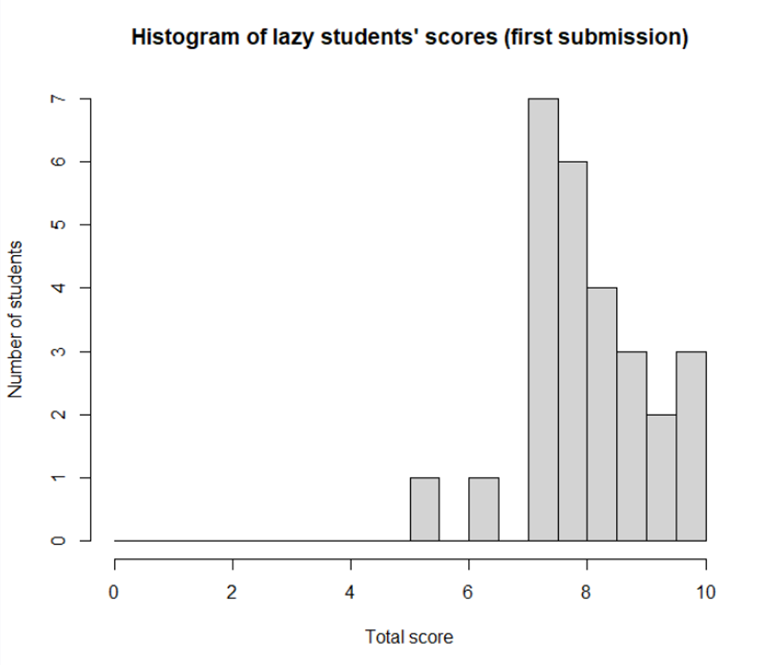
\includegraphics[width = 6 cm]{Images/img7-1-4.png}\\
        Kết quả của quiz 4.2 (điểm lần nộp đầu tiên)
    \end{center}
\end{itemize}
}

%%%%%%%%%%%%%%%%%%%%%%%%%%%%%%%%%%%%%%%%%%%%%%%%%%%%%%%%%%%%%
%%%% Bài 9
\subsection{Bài 9}

\frame
{
\frametitle{Nhóm câu hỏi liên quan đến sinh viên thông minh}
\framesubtitle{Xác định giá trị k và n phù hợp}
\begin{itemize}
    \item Ý tưởng thực hiện: $table(), floor(), order(), match(), min()$
    \item Kết quả:\\
    \begin{center}
        \begin{tabular}{l l c c c} 
             Quiz 1.4 & $\;$ & k = 10, n = 1\\
             Quiz 1.5 & $\;$ & k = 10, n = 1\\
             Quiz 3.3 & $\;$ & k = 10, n = 1\\
             Quiz 4.2 & $\;$ & k = 10, n = 1
        \end{tabular}
    \end{center}
\end{itemize}
}

\frame
{
\frametitle{Nhóm câu hỏi liên quan đến sinh viên thông minh}
\framesubtitle{Xác định số lượng sinh viên thông minh}
\begin{itemize}
    \item Ý tưởng thực hiện: $match(), unique()$
    \item Kết quả:\\
    \begin{center}
        \begin{tabular}{l l c c c} 
             Quiz 1.4 & $\;$ & 91 sinh viên\\
             Quiz 1.5 & $\;$ & 77 sinh viên\\
             Quiz 3.3 & $\;$ & 191 sinh viên\\
             Quiz 4.2 & $\;$ & 29 sinh viên
        \end{tabular}
    \end{center}
\end{itemize}
}

\frame
{
\frametitle{Nhóm câu hỏi liên quan đến sinh viên thông minh}
\framesubtitle{Xác định phổ điểm của các sinh viên thông minh}
\begin{itemize}
    \item Ý tưởng thực hiện: $hist()$
    \item Kết quả:\\
    \begin{center}
        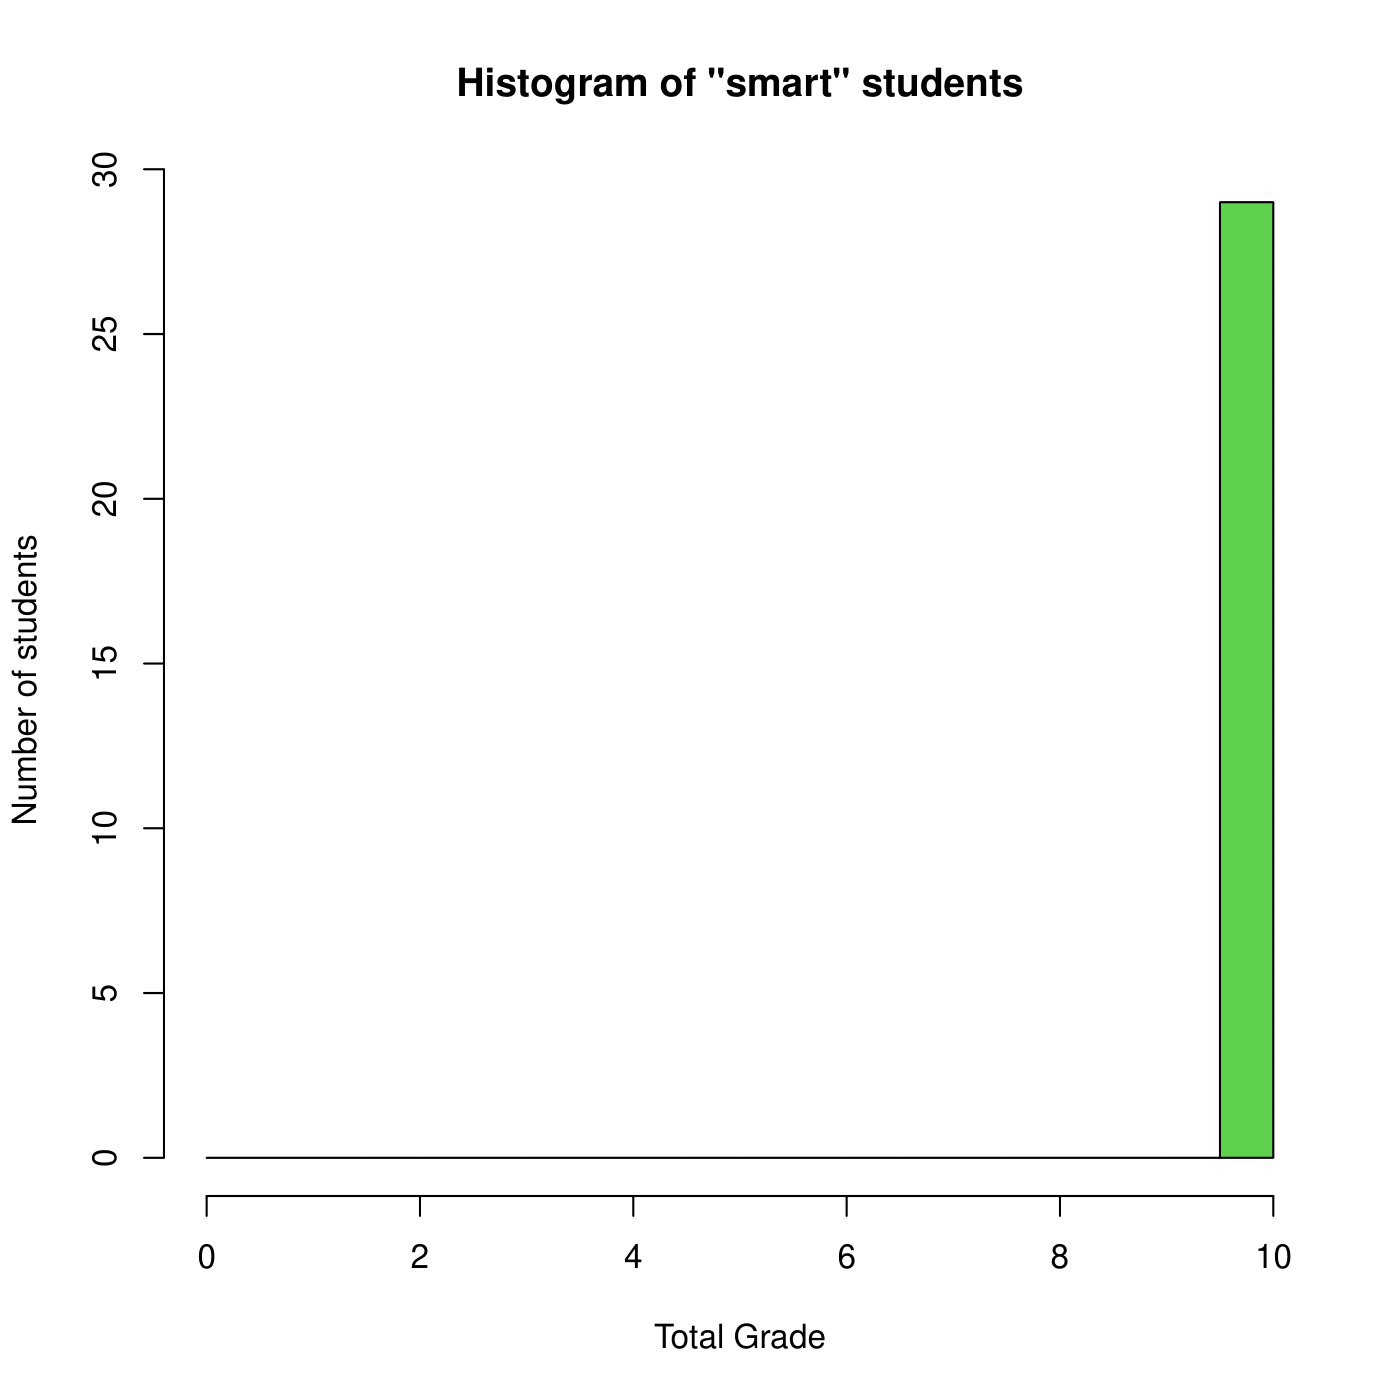
\includegraphics[width = 6 cm]{Images/img9-1-4.png}\\
        Kết quả của quiz 4.2
    \end{center}
\end{itemize}
}

%%%%%%%%%%%%%%%%%%%%%%%%%%%%%%%%%%%%%%%%%%%%%%%%%%%%%%%%%%%%%%%%%%
%%%% Bài 10
\subsection{Bài 10}

\frame
{
\frametitle{Nhóm câu hỏi liên quan đến sinh viên chủ động}
\framesubtitle{Xác định số lượng sinh viên biết cách học chủ động}
\begin{itemize}
    \item Ý tưởng thực hiện: $nrow()$
    \item Kết quả:\\
    \begin{center}
        \begin{tabular}{l l l c c} 
             Quiz 1.4 & $\;$ & $k= 10, n = 1$\\
             & & $t_1 = 19:48$ ngày 25/03/2020\\
             & & $sub = 2$\\
             Quiz 1.5 & $\;$ & $k= 10, n = 1$\\
             & & $t_1 = 22:46$ ngày 27/03/2020\\
             & & $sub = 2$\\
             Quiz 3.3 & $\;$ & $k= 10, n = 1$\\
             & & $t_1 = 20:48$ ngày 13/04/2020\\
             & & $sub = 2$\\
             Quiz 4.2 & $\;$ & $k= 10, n = 1$\\
             & & $t_1 = 13:34$ ngày 17/04/2020\\
             & & $sub = 2$
        \end{tabular}
    \end{center}
\end{itemize}
}

\frame
{
\frametitle{Nhóm câu hỏi liên quan đến sinh viên chủ động}
\framesubtitle{Xác định các thông số $k$, $n$, $t_1$, số lần nộp}
\begin{itemize}
    \item Ý tưởng thực hiện: $order(), ceiling(), subset(), rbind()$
    \item Kết quả:\\
    \begin{center}
        \begin{tabular}{l l c c c} 
             Quiz 1.4 & $\;$ & 111 sinh viên\\
             Quiz 1.5 & $\;$ & 101 sinh viên\\
             Quiz 3.3 & $\;$ & 197 sinh viên\\
             Quiz 4.2 & $\;$ & 49 sinh viên
        \end{tabular}
    \end{center}
\end{itemize}
}

\frame
{
\frametitle{Nhóm câu hỏi liên quan đến sinh viên chủ động}
\framesubtitle{Xác định phổ điểm của các sinh viên biết cách học chủ động}
\begin{itemize}
    \item Ý tưởng thực hiện: $order(), ceiling(), subset(), rbind()$
    \item Kết quả:\\
    \begin{center}
        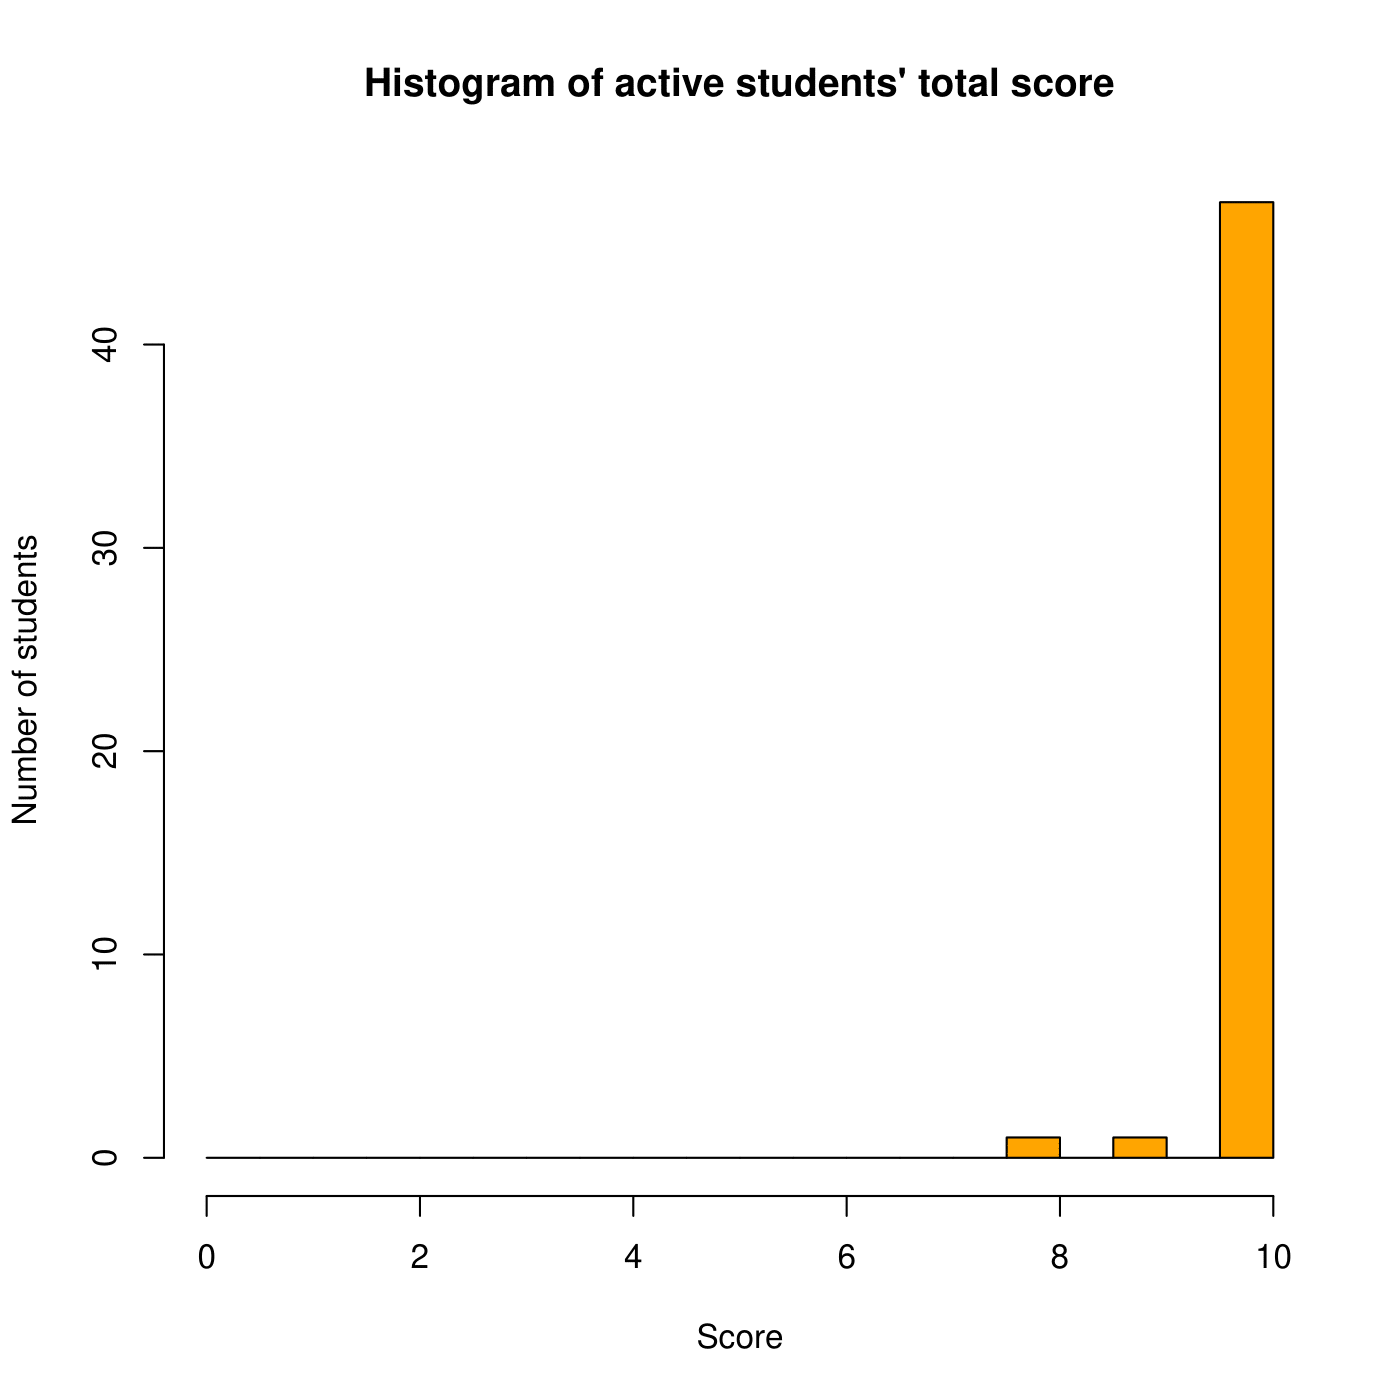
\includegraphics[width = 6 cm]{Images/img10-1-4.png}\\
        Kết quả của quiz 4.2
    \end{center}
\end{itemize}
}

%%%%%%%%%%%%%%%%%%%%%%%%%%%%%%%%%%%%%%%%%%%%%%%%%%%%%%%%%%%%%%%%%%
%%%% Bài 11
\subsection{Bài 11}

\frame
{
\frametitle{Xác định các phần giao của các nhóm sinh viên}
\begin{itemize}
    \item Ý tưởng thực hiện: $subset()$
    \item Kết quả:\\
    \begin{center}
        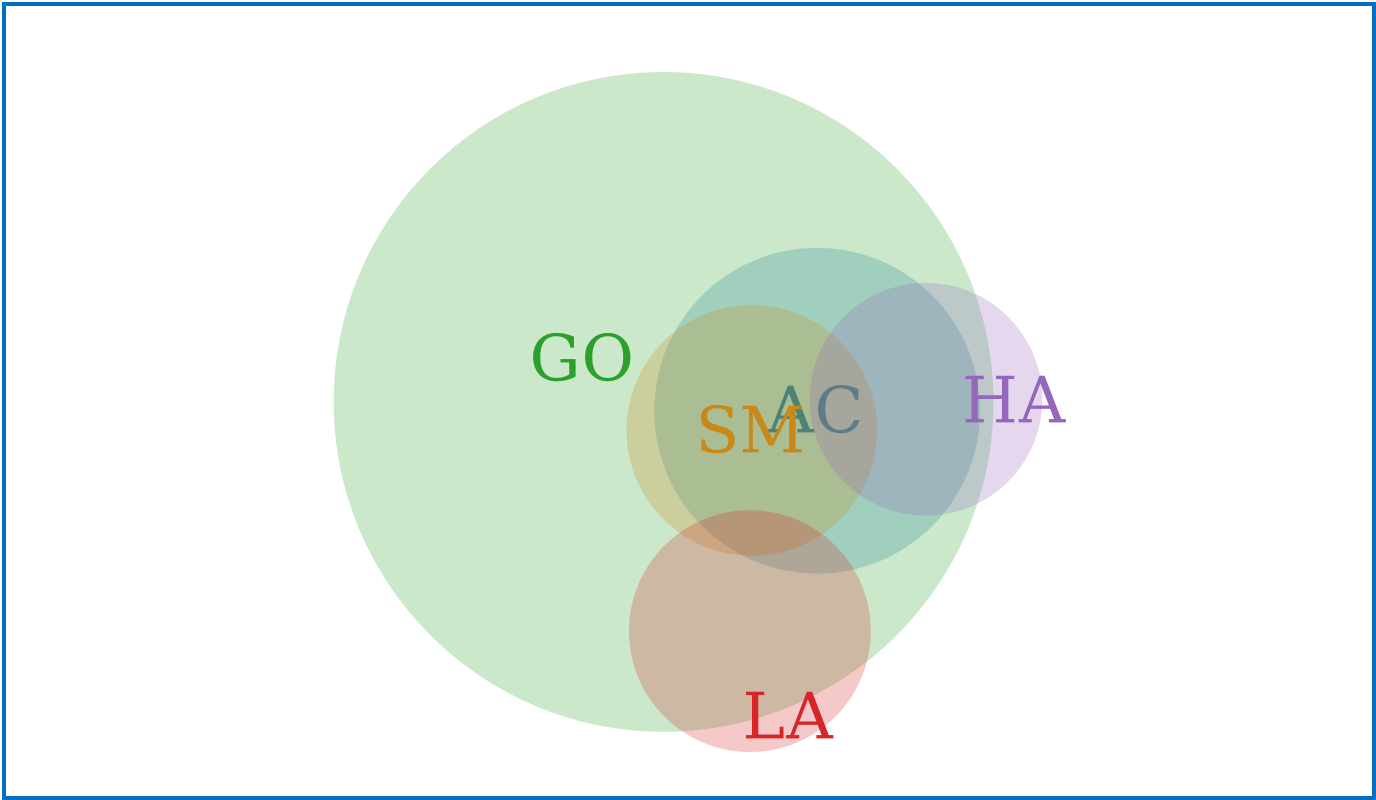
\includegraphics[width = 8 cm]{Images/img11-1-4.png}\\
        Kết quả của quiz 4.2
    \end{center}
\end{itemize}
}

%%%%%%%%%%%%%%%%%%%%%%%%%%%%%%%%%%%%%%%%%%%%%%%%%%%%%%%%%%%%%%%%%%
%%%% Bài 12
\subsection{Bài 12}

\frame
{
\frametitle{Đề xuất, bổ sung một số giá trị thống kê}
\framesubtitle{Xác định phổ thời gian làm bài lần đầu của các sinh viên}
\begin{itemize}
    \item Ý tưởng thực hiện: $hist()$
    \item Kết quả:\\
    \begin{center}
        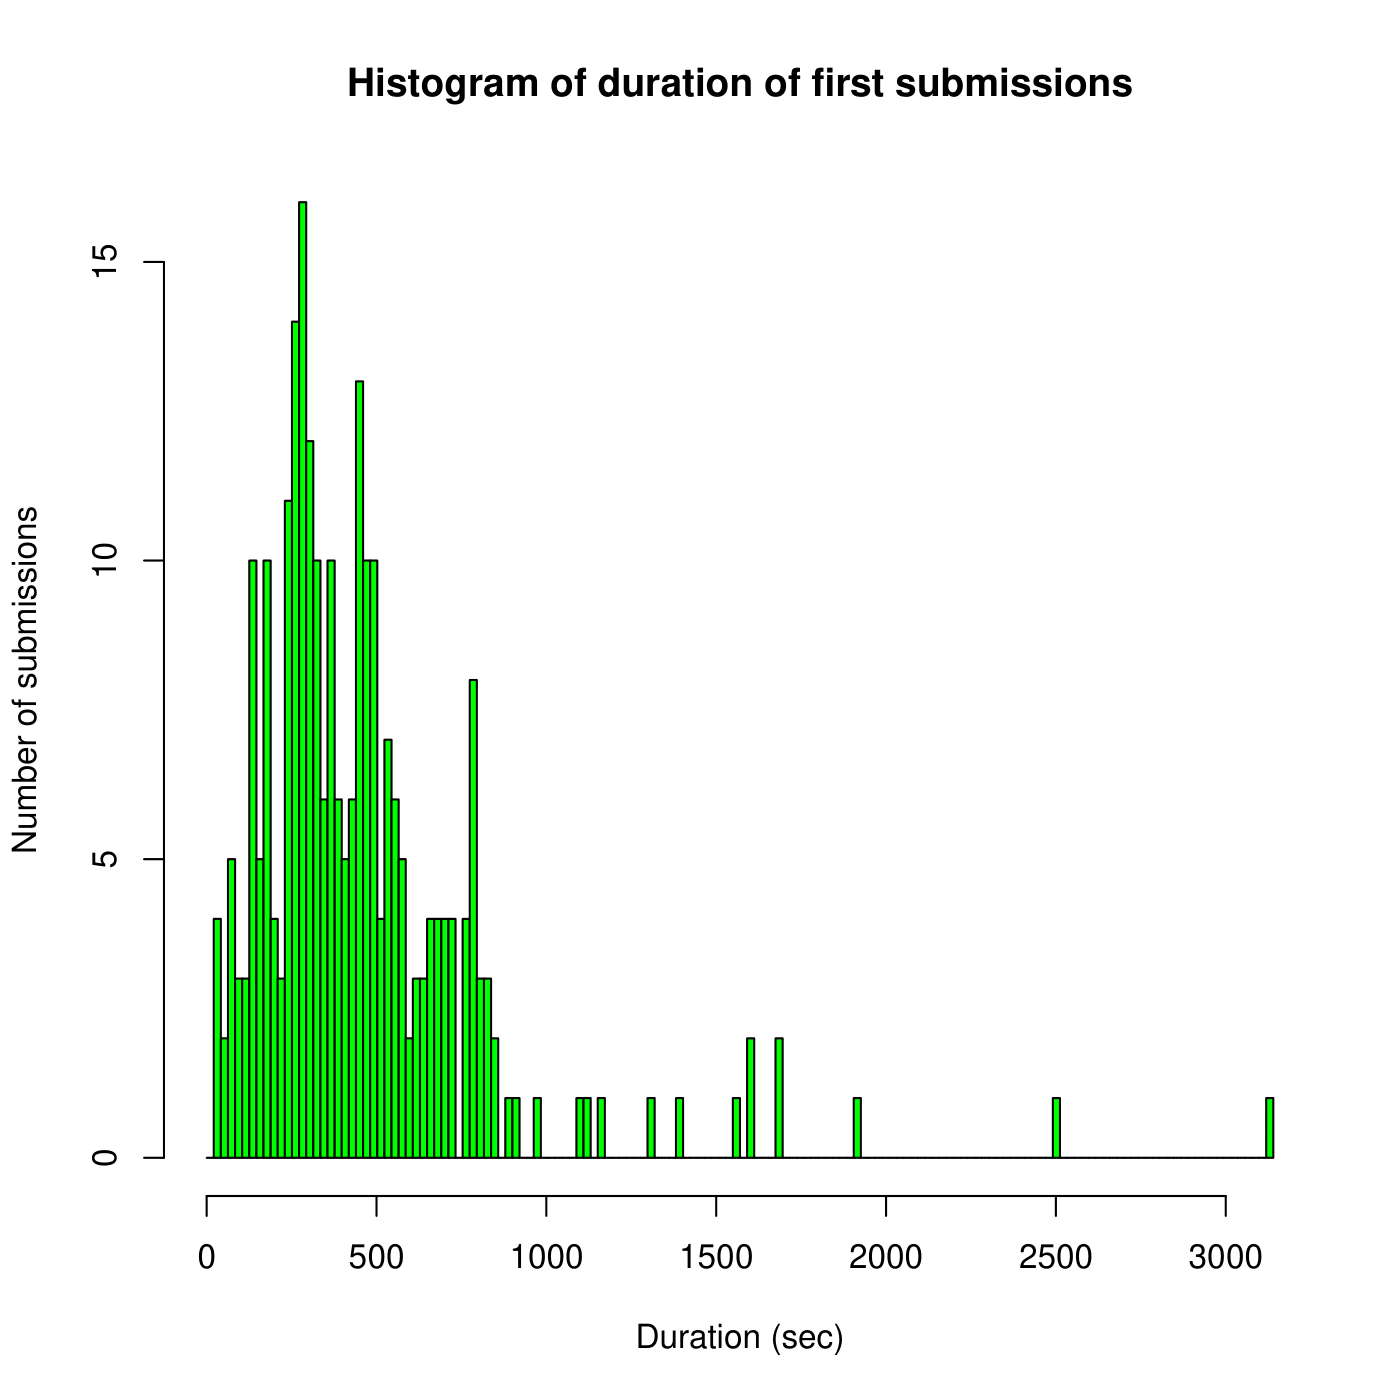
\includegraphics[width = 6 cm]{Images/img12-2-4.png}\\
        Kết quả của quiz 4.2
    \end{center}
\end{itemize}
}

\frame
{
\frametitle{Đề xuất, bổ sung một số giá trị thống kê}
\framesubtitle{Xác định phổ thời gian làm bài lần cuối của các sinh viên}
\begin{itemize}
    \item Ý tưởng thực hiện: $hist()$
    \item Kết quả:\\
    \begin{center}
        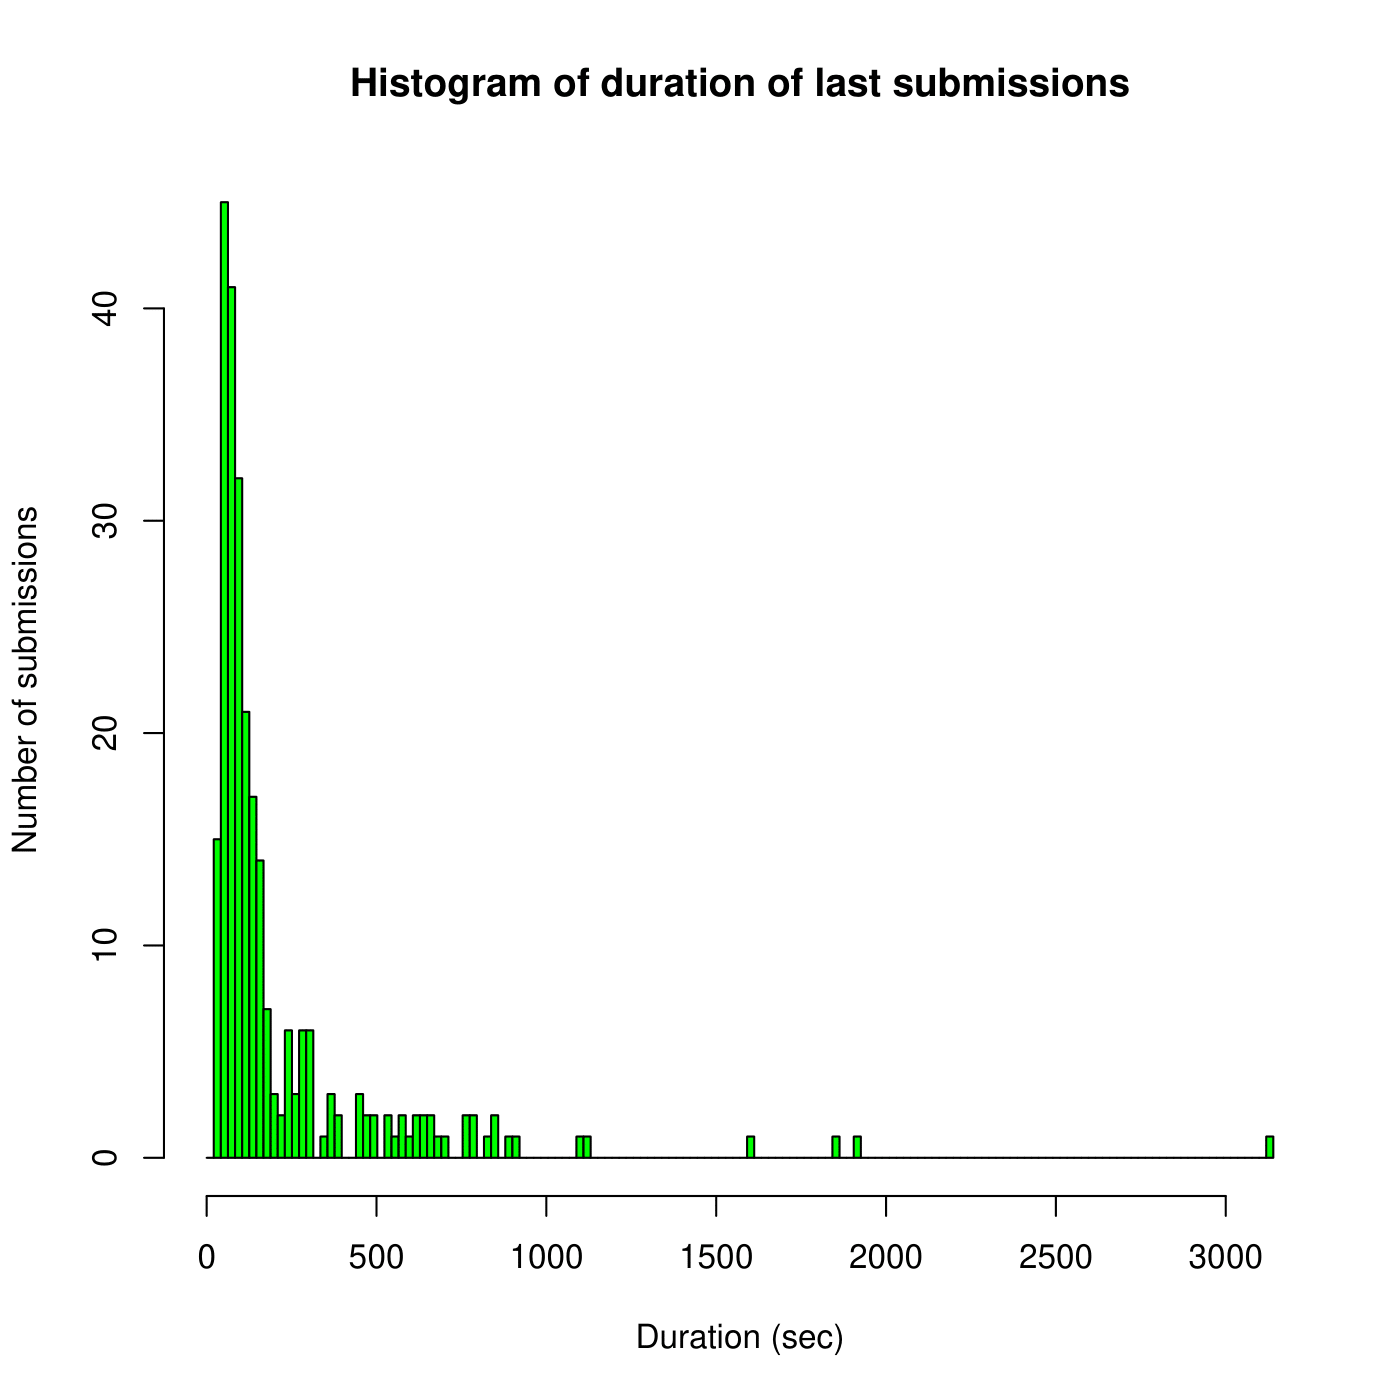
\includegraphics[width = 6 cm]{Images/img12-3-4.png}\\
        Kết quả của quiz 4.2
    \end{center}
\end{itemize}
}

\frame
{
\frametitle{Đề xuất, bổ sung một số giá trị thống kê}
\framesubtitle{Xác định phổ thời gian làm bài lần đầu của các sinh viên có 2 lần nộp bài trở lên}
\begin{itemize}
    \item Ý tưởng thực hiện: $hist()$
    \item Kết quả:\\
    \begin{center}
        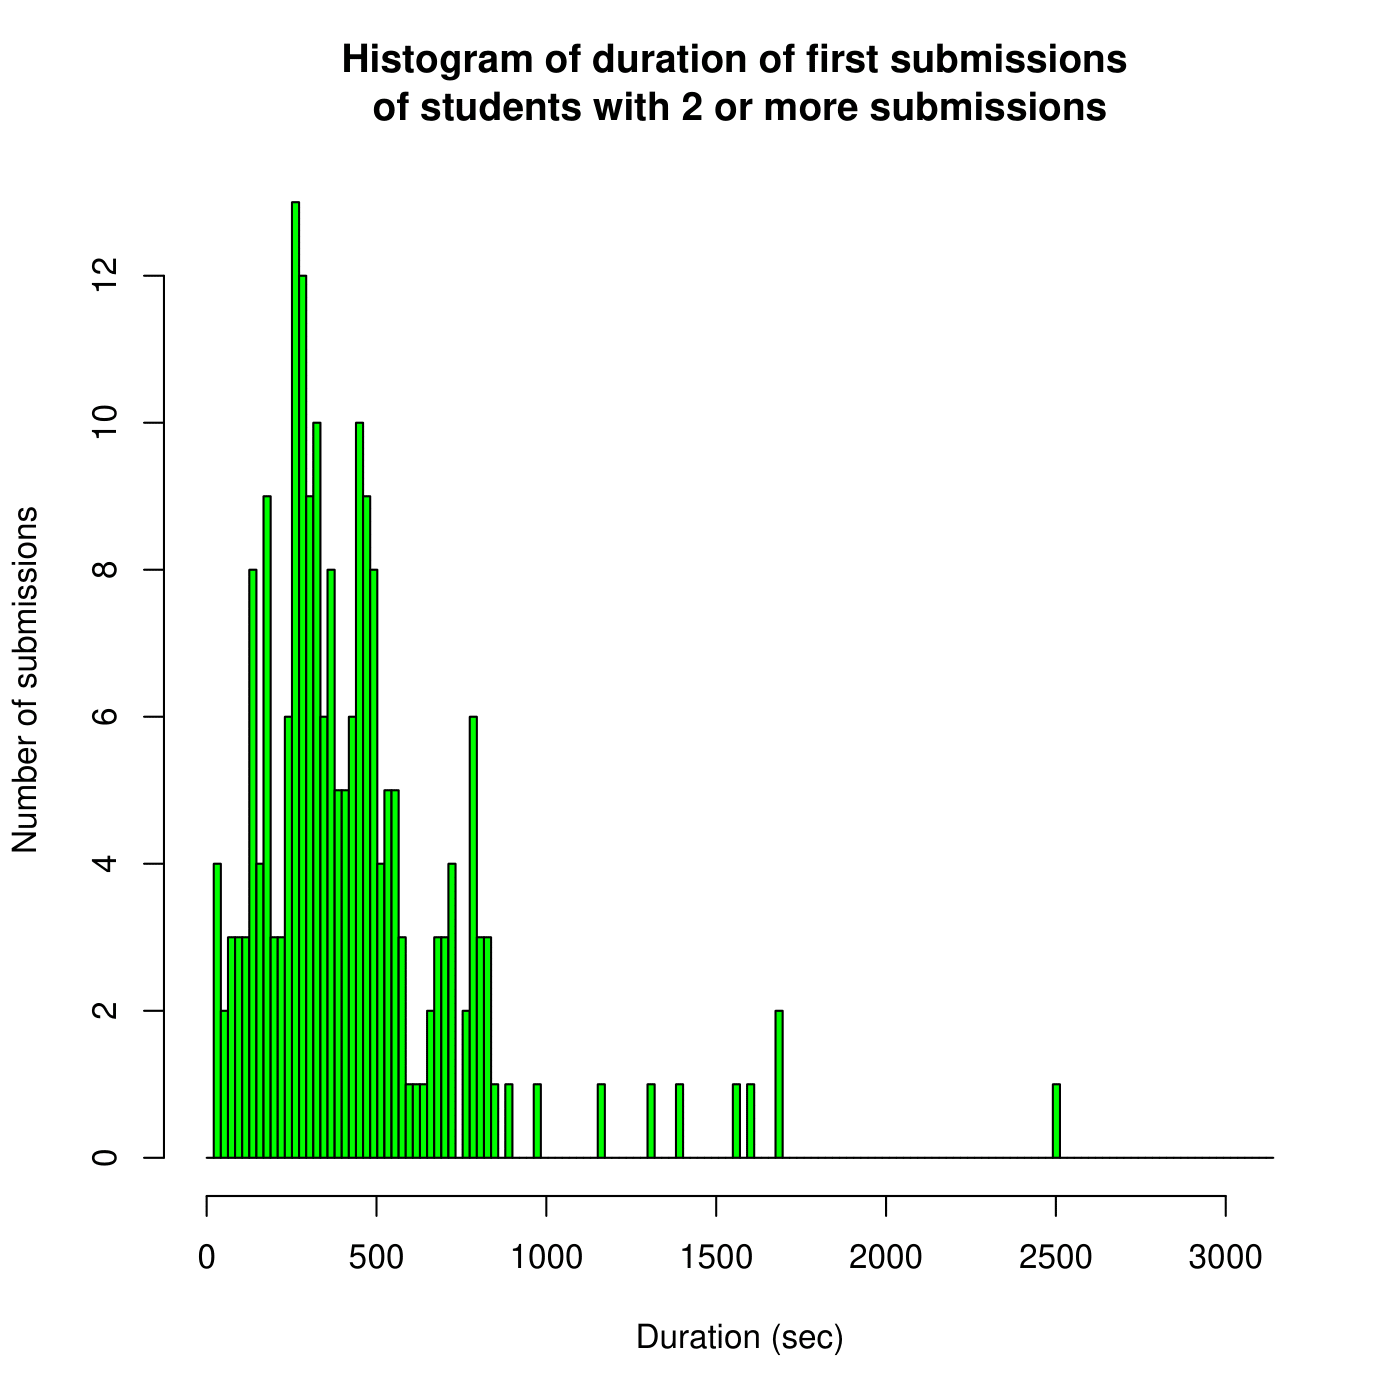
\includegraphics[width = 6 cm]{Images/img12-4-4.png}\\
        Kết quả của quiz 4.2
    \end{center}
\end{itemize}
}

\frame
{
\frametitle{Đề xuất, bổ sung một số giá trị thống kê}
\framesubtitle{Xác định phổ thời gian làm bài lần cuối của các sinh viên có 2 lần nộp bài trở lên}
\begin{itemize}
    \item Ý tưởng thực hiện: $hist()$
    \item Kết quả:\\
    \begin{center}
        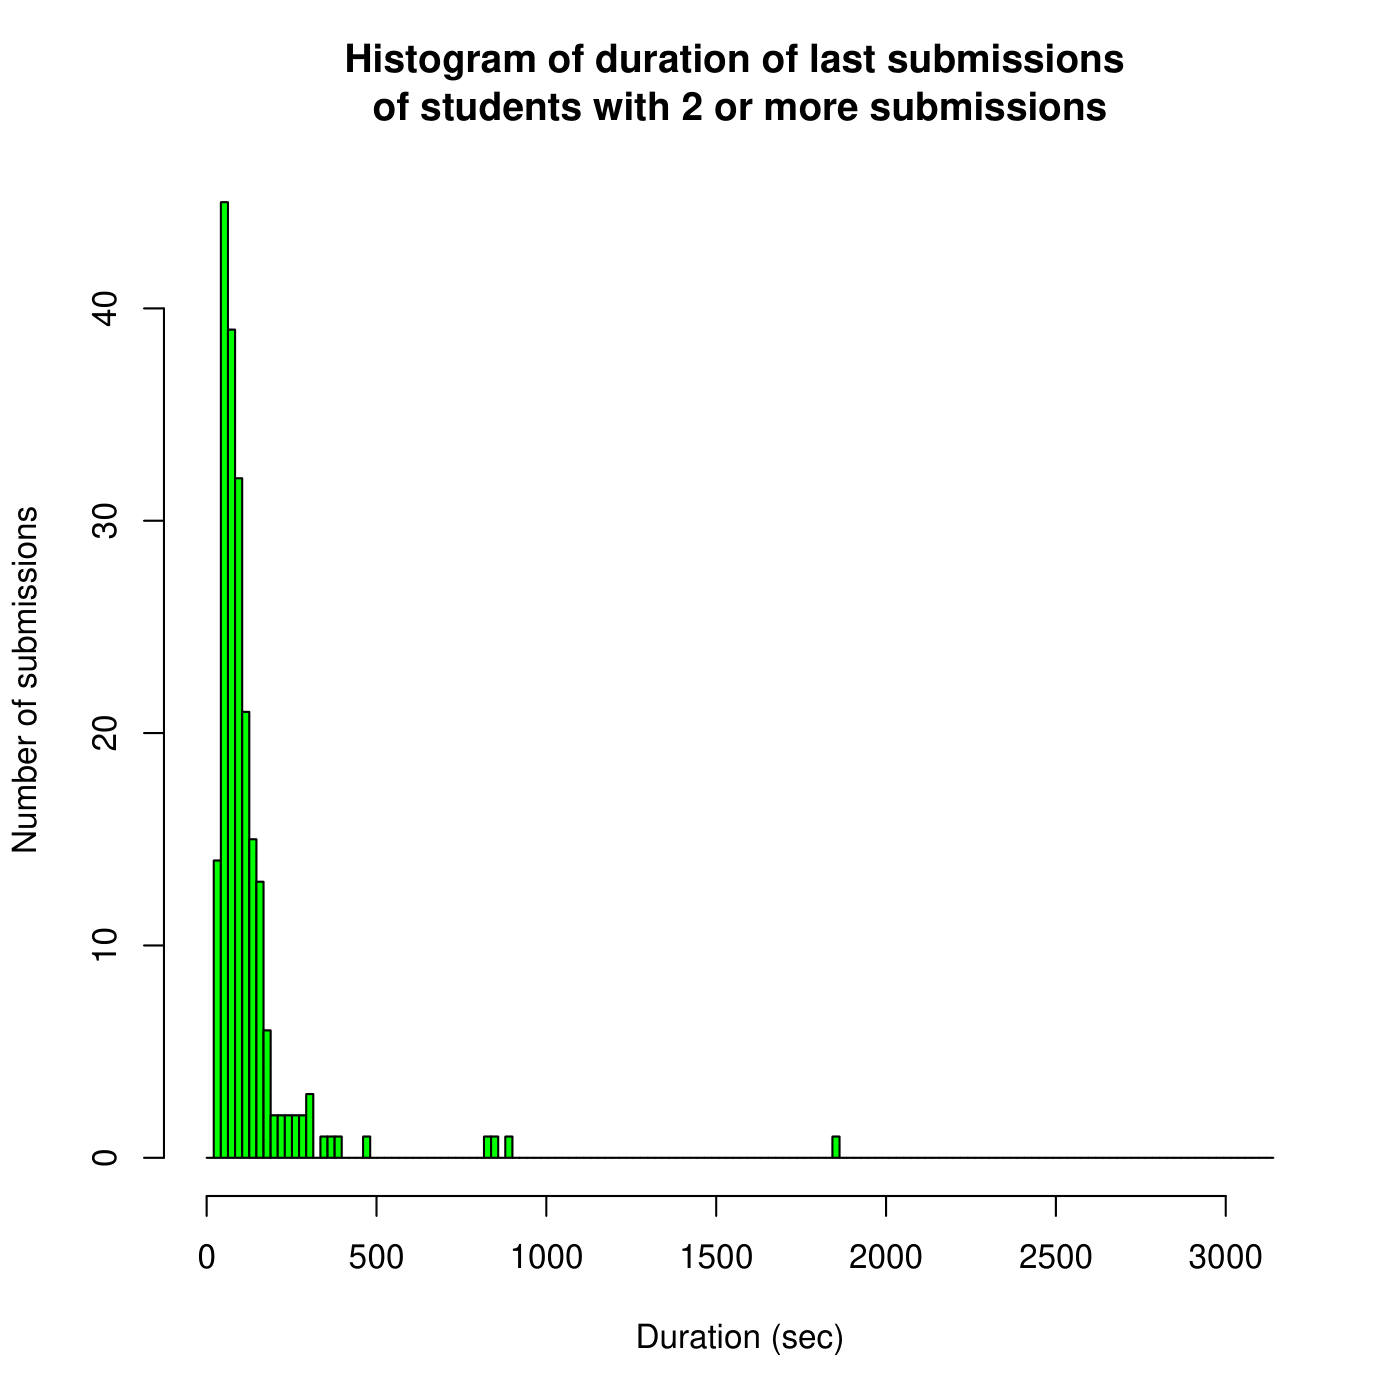
\includegraphics[width = 6 cm]{Images/img12-5-4.png}\\
        Kết quả của quiz 4.2
    \end{center}
\end{itemize}
}

\frame
{
\frametitle{Đề xuất, bổ sung một số giá trị thống kê}
\framesubtitle{Xác định thời gian làm bài trung bình của các sinh viên có 2 lần nộp bài trở lên}
\begin{itemize}
    \item Ý tưởng thực hiện: $hist()$
    \item Kết quả:\\
    \begin{center}
        \begin{tabular}{l l c c c} 
             & & Lần đầu & Lần cuối\\
             Quiz 1.4 & $\;$ & 470.32 s & 95.115 s\\
             Quiz 1.5 & $\;$ & 707.831 s & 144.9624 s\\
             Quiz 3.3 & $\;$ & 288.2 s & 60.65714 s\\
             Quiz 4.2 & $\;$ & 438.1214 s & 123.8204 s
        \end{tabular}
    \end{center}
\end{itemize}
}

\frame
{
\frametitle{Đề xuất, bổ sung một số giá trị thống kê}
\framesubtitle{Xác định phổ điểm lần đầu của các sinh viên có 2 lần nộp bài trở lên}
\begin{itemize}
    \item Ý tưởng thực hiện: $hist()$
    \item Kết quả:\\
    \begin{center}
        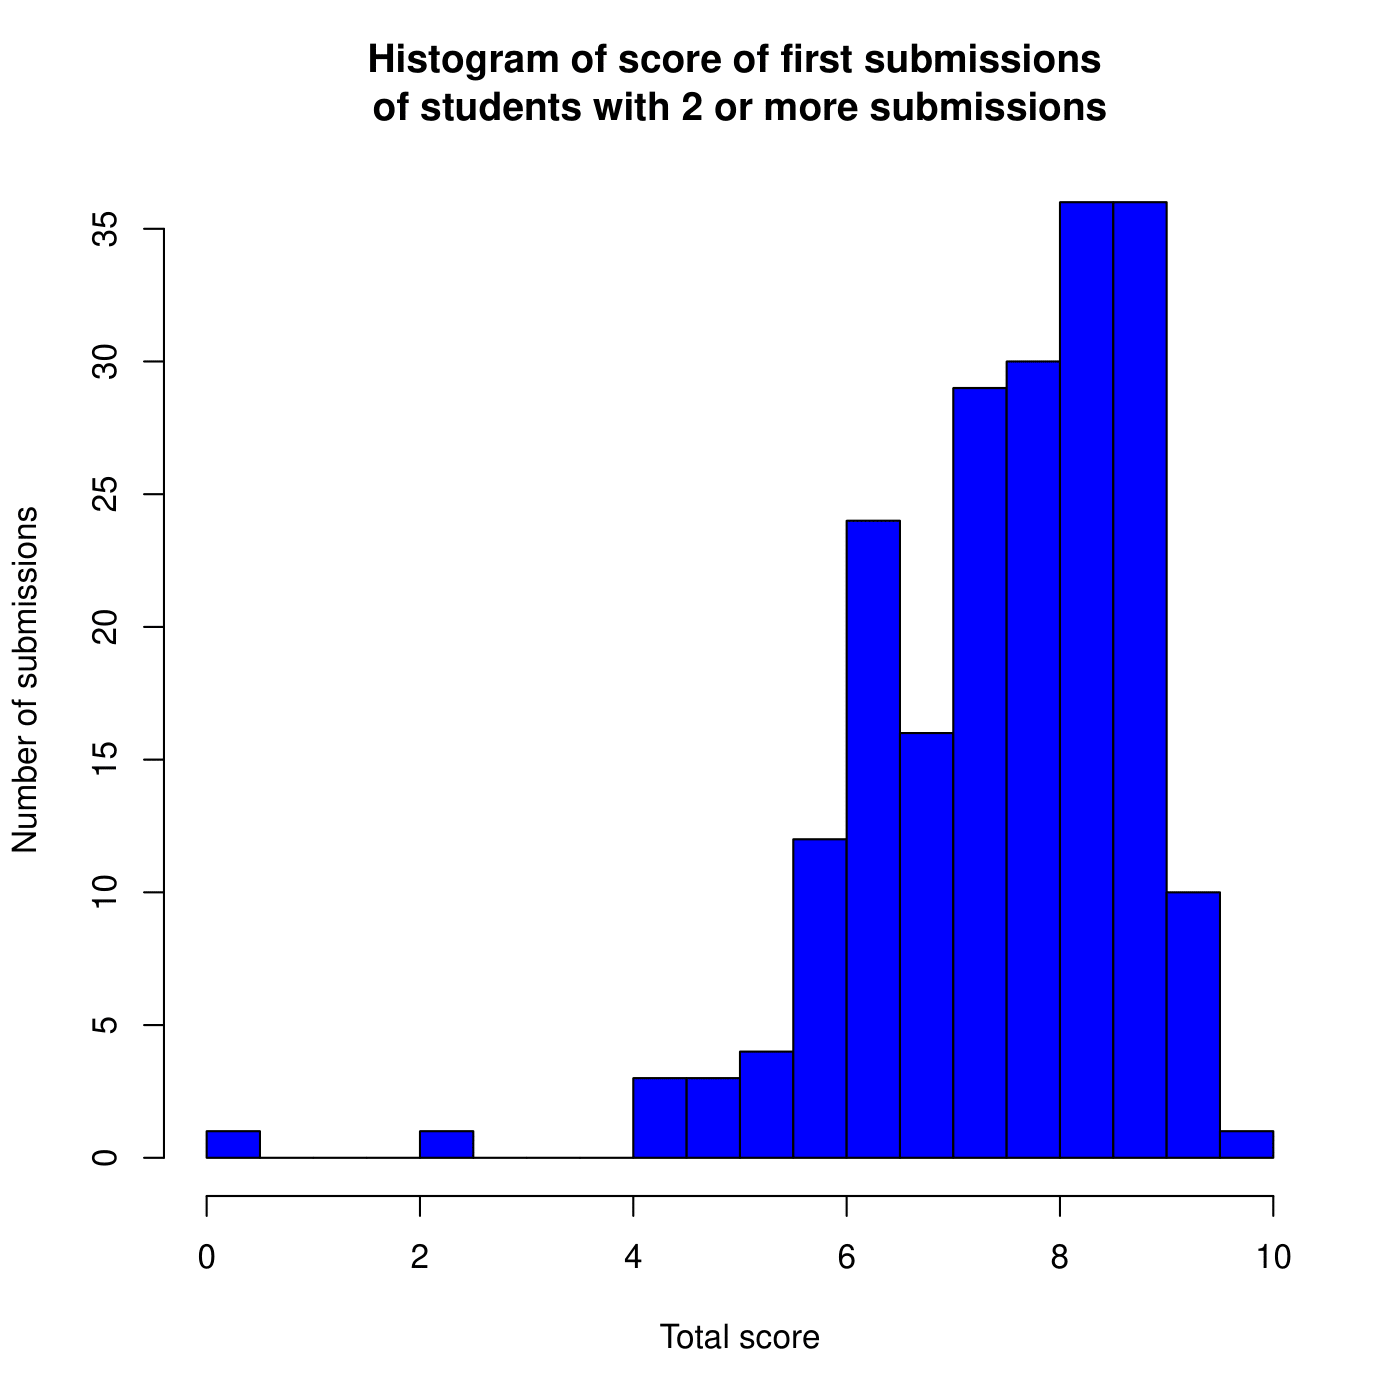
\includegraphics[width = 6 cm]{Images/img12-6-4.png}\\
        Kết quả của quiz 4.2
    \end{center}
\end{itemize}
}

\frame
{
\frametitle{Đề xuất, bổ sung một số giá trị thống kê}
\framesubtitle{Xác định phổ điểm lần cuối của các sinh viên có 2 lần nộp bài trở lên}
\begin{itemize}
    \item Ý tưởng thực hiện: $hist()$
    \item Kết quả:\\
    \begin{center}
        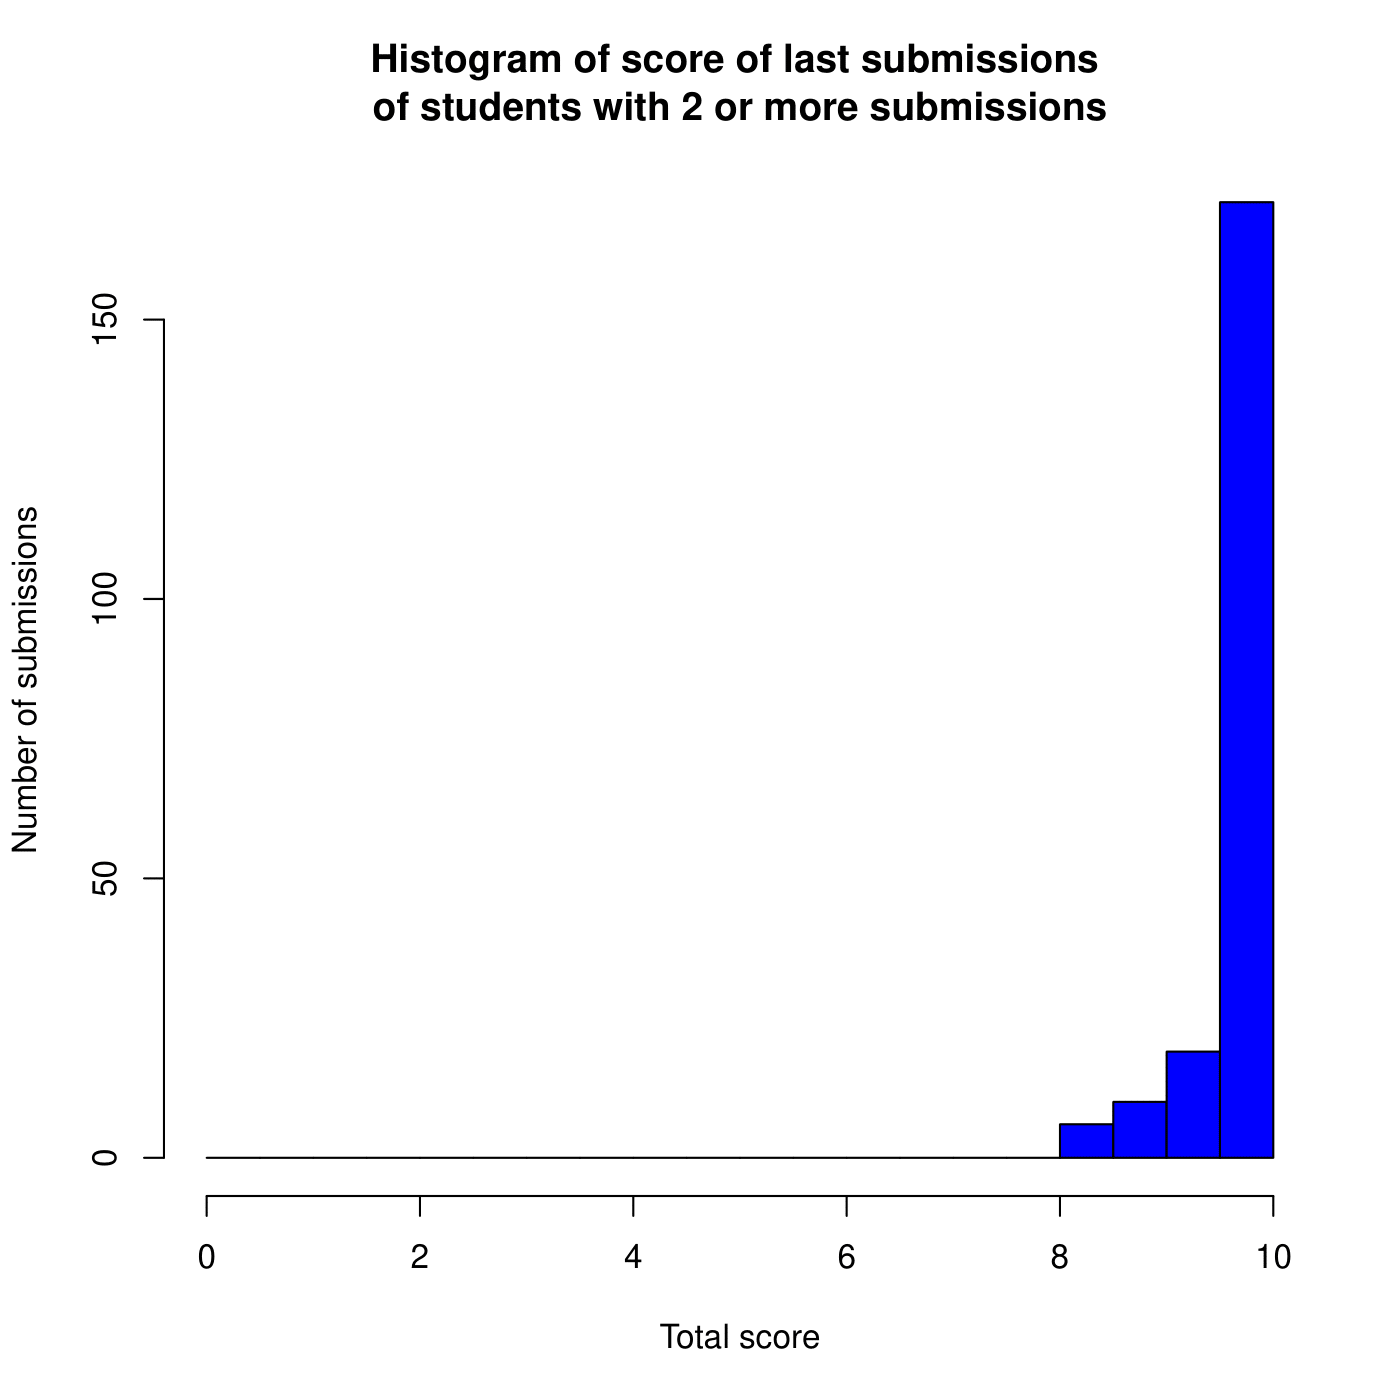
\includegraphics[width = 6 cm]{Images/img12-7-4.png}\\
        Kết quả của quiz 4.2
    \end{center}
\end{itemize}
}

\end{document}

